% =============================================================================
% SwantonRanch_LTE.tex
% Senior Project Report: Swanton Pacific Ranch Private LTE Network
% California Polytechnic State University, San Luis Obispo
% EE 461 / EE 462 -- Spring 2026
% =============================================================================

\documentclass[
    left=1.5in,
    right=1.25in,
    top=1.25in,
    bottom=1.25in
]{CalPolySeniorProject}

% -----------------------------------------------------------------------------
% Metadata
% -----------------------------------------------------------------------------
\setprojecttitle{Swanton Pacific Ranch Private LTE Network:\\[0.4em]
    \large Design, Simulation, and Deployment of a CBRS Band~48
    Private Cellular Network}
\setauthor{1}{Gregory Karaoghlanian}{gkaraogh@calpoly.edu}
\setauthor{2}{Frankie Medrano}{fjmedran@calpoly.edu}
\setauthor{3}{AJ Gregory}{agrego10@calpoly.edu}
\setprofessor{Faculty Advisor: Dr.\ Dennis Derickson \quad
    Industry Mentor: Jonathan Polly}
\setclass{EE 461 / EE 462}
\setdepartment{Electrical Engineering Department}
\setquarter{Spring 2026}

\addbibresource{Sources.bib}

% Override cpspextraauthorrows to directly output author 3.
\renewcommand{\cpspextraauthorrows}{%
    \\ \addlinespace[1em]%
    \authorrow{3}%
}

% Override maketitlepage to keep everything on one page (single-spaced,
% tighter vertical spacing, slightly smaller logo).
\renewcommand{\maketitlepage}{%
    \hypersetup{pageanchor=false}%
    \begin{titlepage}
        \setstretch{1}%
        \centering

        {\Huge\bfseries \projecttitle\par}
        \vspace*{3.5em}

        {\Large\scshape \class\par}%
        \rule{\linewidth}{0.35mm}
        \par\vspace*{1em}

        \begin{tabular}{r | l}
            \authorrow{1}%
            \ifcsname author2Name\endcsname
                \\ \addlinespace[1em]
                \authorrow{2}%
            \fi
            \cpspextraauthorrows
        \end{tabular}%

        \par\vspace{1em}%
        \rule{\linewidth}{0.35mm}%
        \par\vspace{2em}%

        
\includegraphics[width=0.50\textwidth]{Images/Logo.pdf}\par
        \vspace*{1.5em}

        \begin{minipage}{\textwidth}
            \centering
            {\large Faculty Advisor: Dr.\ Dennis Derickson}\par
            \vspace{8pt}
            {\large Industry Mentor: Jonathan Polly}\par
            \vspace{10pt}
            {\large \department}\par
            \vspace{10pt}
            {\Large California Polytechnic State University}\par
            \vspace{10pt}
            {\small San Luis Obispo \textendash~\quarter}\par
        \end{minipage}

        \vfill
    \end{titlepage}%
    \hypersetup{pageanchor=true}%
}

% Extra packages useful for this report
\usepackage{enumitem}
\usepackage{tabularx}
\usepackage{multirow}

\begin{document}

% -----------------------------------------------------------------------------
% Title page
% -----------------------------------------------------------------------------
\maketitlepage

% -----------------------------------------------------------------------------
% Front matter
% -----------------------------------------------------------------------------
\pagenumbering{roman}
\pagestyle{plain}

% Statement of Disclaimer
\section*{Statement of Disclaimer}
\addcontentsline{toc}{section}{Statement of Disclaimer}

\textit{Since this project is a result of a class assignment, it has been
graded and accepted as fulfillment of the course requirements. Acceptance does
not imply technical accuracy or reliability. Any use of information in this
report is done at the risk of the user. These precautions have been taken to
achieve a high quality report:}

\textit{This report has been subject to peer review, advisor review, and
industry mentor review. All technical claims have been verified against
manufacturer documentation, measured field data, and published references.
Equipment specifications are cited from official product documentation. Field
measurement data is preserved in its original form in the project repository.}

% Table of Contents
\clearpage
\tableofcontents

\clearpage
\listoffigures
\addcontentsline{toc}{section}{List of Figures}

\clearpage
\listoftables
\addcontentsline{toc}{section}{List of Tables}

% Acknowledgements
\clearpage
\section*{Acknowledgements}
\addcontentsline{toc}{section}{Acknowledgements}

The team thanks Jonathan Polly, Chief Technologist at the Cal Poly 5G
Innovation Lab and Digital Transformation Hub, for providing sustained
technical mentorship throughout the project and for sharing his industry
expertise during every phase from concept to report. His guidance on network
architecture, equipment selection, and the broader context of private cellular
made this project substantially richer than it would have been otherwise.

Thanks to Mark Houtz for sharing his deep expertise on CBRS and private LTE,
for making the WLPC Phoenix 2026 course materials available to the team, and
for his blog and community resources that served as a practical foundation for
the lab build.

Thanks to Mark Swisher, ranch manager at Swanton Pacific Ranch, for hosting
the team during the deployment, providing access to the site, and sharing his
perspective on the connectivity challenges the ranch faces every day.

The team is grateful to Lawrence Berkeley National Laboratory for donating the
Baicells Nova 846 eNodeB and Alpha Wireless AW3376-E-F sector antenna that made
the Swanton deployment possible.

Thanks to Dr.\ Dennis Derickson for advising this project and for giving the
team the freedom to approach it in a way that was both technically rigorous and
genuinely interesting.

% Abstract
\clearpage
\section*{Abstract}
\addcontentsline{toc}{section}{Abstract}

Cal Poly's Swanton Pacific Ranch, a 3,200-acre working ranch and student
research facility in Davenport, California, lost most of its communication
infrastructure in the 2020 CZU Lightning Complex fires. Six years later, the
ranch operates with only a solar-powered UHF voice repeater and a fiber
connection to the bunkhouse. Commercial cellular coverage across the property
is extremely limited. As Cal Poly moves toward year-round student residents and
expanded research programs at the site, the need for a robust communication
network has only grown since the fires.

This project designed, simulated, and deployed a private 4G LTE network at the
ranch using the Citizens Broadband Radio Service (CBRS) Band~48 spectrum. The
hardware consisted of a Baicells Nova 846 outdoor macro eNodeB paired with an
Alpha Wireless AW3376-E-F 8-port sector antenna, both donated by Lawrence
Berkeley National Laboratory, and an Intel NUC running Open5GS as the LTE core
network. Custom SIM cards provisioned with PLMN 315-010 authenticated three
Android test devices. Starlink provided internet backhaul at the deployment
site.

Before deployment, the team used eino.ai, a cloud-native RF propagation
simulation tool, to model coverage from Cooke's Peak, the site's highest
elevation point. The simulation guided the sector heading, antenna
configuration, and expectations for coverage extent.

The network went live on May 2, 2026. Three users carried Android phones
running G-NetTrack Lite, collecting 1,655 valid RSRP measurements from the
\textit{Swanton\_Ranch} network across approximately 4~km of terrain. Strong
signal was measured near the radio at Cooke's Peak, degrading to marginal at
range. The simulation correctly identified the coverage direction and near-field
performance, but overestimated the effective coverage radius, a discrepancy
attributed primarily to antenna gain and environmental factors.

The result is a functional, documented private LTE network at Swanton Ranch and
a complete technical foundation for future student teams to build a permanent
installation. This project demonstrates that a university team can deploy
enterprise-grade private cellular infrastructure with open-source software,
commodity hardware, and freely available spectrum at a fraction of traditional
cost.

% -----------------------------------------------------------------------------
% Main matter
% -----------------------------------------------------------------------------
\clearpage
\pagenumbering{arabic}
\setcounter{page}{1}

% =============================================================================
\section{Introduction}
% =============================================================================

\subsection{The Growth of Cellular Networks}

Something has shifted in how the physical world connects. For the first three
decades of the cellular era, the primary use case was personal
connectivity---a person carrying a handset, making calls, sending messages.
That framing made sense when cellular networks were expensive to build, spectrum
was licensed in large blocks at auction, and the hardware required to run a base
station cost millions of dollars and filled a climate-controlled equipment room.

That framing no longer fits the technology. What has emerged is a fundamentally
different model, one where the radio infrastructure itself has become a platform
for machine communication at scale. Autonomous ground vehicles navigating
warehouse floors, security cameras streaming high-definition video across
industrial facilities, IoT sensors monitoring soil moisture and cattle locations
across thousands of acres, precision irrigation controllers responding to
real-time field data: none of these applications fit the mold of personal
connectivity, and most of them cannot be reliably served by Wi-Fi.

Wi-Fi was designed for local, fixed-location coverage. It handles shared access
through contention protocols that work well with a small number of devices in a
controlled indoor environment. At field scale, across kilometers of complex
terrain, with devices moving at vehicle speed, Wi-Fi's limitations become
structural. Range is limited. Interference compounds as device counts grow.
There is no quality-of-service guarantee, which matters when a machine control
system shares the air with consumer traffic. There is no built-in mobility
management, so handoffs between access points are unreliable. Wi-Fi was built
for a specific problem, and it solves that problem well. The problem at Swanton
Ranch is different.

Cellular networks, by contrast, were designed from the ground up for wide-area
coverage, mobility, deterministic quality of service, and strong security. The
challenge has historically been cost: building and operating a cellular network
required carrier-scale investment. That barrier has now substantially fallen,
and the reasons are worth understanding because they explain why this project
was possible at all.

Three things changed in parallel. First, the standardization of open-source
core network software, most notably Open5GS, made it possible to run a fully
functional LTE Evolved Packet Core on commodity server hardware for free. The
software that once ran only on purpose-built telecom equipment now runs in a
Docker container on a laptop. Second, companies like Baicells brought commodity
eNodeB hardware to market at price points accessible to enterprises and
universities, hardware that would have cost hundreds of thousands of dollars a
decade ago. Third, the Citizens Broadband Radio Service opened 150~MHz of
mid-band spectrum in the 3.5~GHz band to shared use without requiring a
traditional spectrum license. Any organization can access this spectrum, deploy
a private network, and operate it without negotiating with a carrier.

The convergence of free software, affordable hardware, and accessible spectrum
means that private cellular is no longer a solution only for large enterprises
with dedicated telecom engineering teams. Organizations with modest budgets and
the technical staff to configure and maintain the system can now deploy and
operate their own LTE networks. The tools are accessible, the knowledge is
documented, and the demand is real.

\subsection{The Opportunity at Swanton Pacific Ranch}

Cal Poly's Swanton Pacific Ranch sits on 3,200 acres of coastal terrain in
Davenport, California, roughly ten miles north of Santa Cruz. The ranch was
donated to Cal Poly in 1993 and has operated since then as a working ranch and
student research facility, hosting programs across agriculture, natural
resources, and biological sciences. It is one of several Cal Poly Learn By
Doing field sites that give students hands-on experience with working systems
and real environments.

In August 2020, the CZU Lightning Complex fires burned across Santa Cruz and
San Mateo counties. At Swanton Ranch, roughly 80 percent of the 3,200 acres
burned. The fire destroyed research infrastructure, equipment, and fencing. It
also destroyed an AT\&T fiber optic cable that had been buried underground. That
cable was the ranch's primary connection to the outside world
\autocite{hayes2020swanton}.

After the fire, the ranch was left with two communication options. The first
was a UHF voice repeater on Cooke's Peak, the dominant high point on the
property, which provides solar-powered walkie-talkie connectivity across the
ranch but no data capability. The second was a fiber optic connection to the
bunkhouse, the ranch's main living and working facility, which provides internet
access at that one location but nowhere else on the property. Commercial
cellular coverage across the ranch is extremely limited. While the drive test
data captured occasional brief signals from T-Mobile, AT\&T, and Verizon at
isolated points along the test route, no carrier provides usable coverage across
the full working areas of the property.

The consequences of this gap are already visible. Cal Poly's BRAE department
(BioResource and Agricultural Engineering) deployed IoT gateways at Swanton to
support environmental monitoring research. Those gateways could not register on
commercial SIM cards because there is no usable commercial coverage at the site.
The devices sat unused, not because of a hardware failure or a configuration
error, but simply because there was no network for them to connect to. This is
precisely the scenario that private cellular addresses. A provisioned SIM on the
project's network would have allowed those gateways to connect immediately,
without any dependency on a commercial carrier.

Cal Poly is planning to expand both the student population and the research
scope at the ranch, moving toward year-round habitation. That plan requires
reliable communication. Voice-only UHF coverage, adequate for a day-trip
working environment, is not sufficient infrastructure for a facility with
resident students, active research instruments, livestock monitoring, and the
safety obligations that come with extended human presence on a remote rural
property.

The project team set out to provide the first step toward that infrastructure: a
working private LTE network at Swanton that could demonstrate feasibility,
characterize coverage, and leave behind a complete technical foundation for the
student teams that follow.

% =============================================================================
\section{Background}
% =============================================================================

\subsection{Agricultural Technology: Use Cases at Swanton Ranch}

Modern working ranches generate and consume data across a wide range of
operations, and the value of that data depends entirely on whether it can be
collected, transmitted, and acted on in real time. At a site like Swanton Ranch,
the specific connectivity use cases are well-defined. Seawater intrusion
monitoring, which tracks saltwater movement into agricultural aquifers along the
coast, requires frequent automated readings from sensors distributed across the
property. Flow meters on irrigation systems generate continuous data that can
reduce water consumption and detect leaks before they become expensive.
GPS-based livestock tracking allows ranchers to locate animals and detect
behavioral anomalies without physically walking the property. Lifecycle
monitoring for livestock health and breeding management requires connectivity to
be useful at scale. Larger bandwidth use cases include security cameras
protecting equipment and structures, environmental sensors for the research
programs hosted at the ranch, and basic voice and data connectivity for students
and staff working at remote locations \autocite{polly2024agtech}.

At present, none of these capabilities exist at Swanton Ranch outside the
bunkhouse. The UHF voice repeater supports voice only. The fiber connection at
the bunkhouse is geographically fixed. The gap between what modern agricultural
research requires and what the ranch's current infrastructure provides is the
central motivation for this project.

\subsection{Swanton Pacific Ranch: Site and Terrain}

Swanton Pacific Ranch occupies 3,200 acres of coastal terrain in Santa Cruz
County, California. The property runs from the Pacific Ocean shoreline eastward
into the Santa Cruz Mountains, with Highway~1 passing through the western
portion of the ranch near the coast.

The terrain is characteristic of the central California coast: steep ridgelines
running roughly north-south, with narrow valleys carved by seasonal streams.
Cooke's Peak is the dominant high point on the property, rising to approximately
243 meters above sea level. From Cooke's Peak, the ranch valley opens to the
south and east, with the coastal bluffs and the ocean visible to the west. Dense
groves of coastal Douglas-fir occupy the slopes, providing windbreak but also
attenuating radio signals through foliage.

The 2020 fires burned through most of the ranch. Six years later, the property
is in active recovery, with some areas showing regrowth while others retain the
standing dead timber characteristic of fire-killed conifer forests. This
vegetation pattern affects radio propagation: recovering brush and standing dead
wood present different attenuation characteristics than the mature forest that
existed before the fire, and both differ from what a propagation model
calibrated on pre-fire imagery would predict.

Figure~\ref{fig:topo} shows the USGS 7.5-minute topographic map of the Swanton
Ranch area at 1:24,000 scale \autocite{usgs2026topo}. The map shows the terrain
that governs line-of-sight from Cooke's Peak to different parts of the ranch.
The valley floor south of Cooke's Peak lies in partial shadow from the ridge,
and the terrain to the east rises again before reaching the ranch boundary. This
topographic structure was the primary factor driving the simulation work
described in Section~IV.D, and it directly explains why signal measured from a
single radio at Cooke's Peak degrades rapidly with distance in certain
directions.

\begin{figure}[!ht]
    \centering
    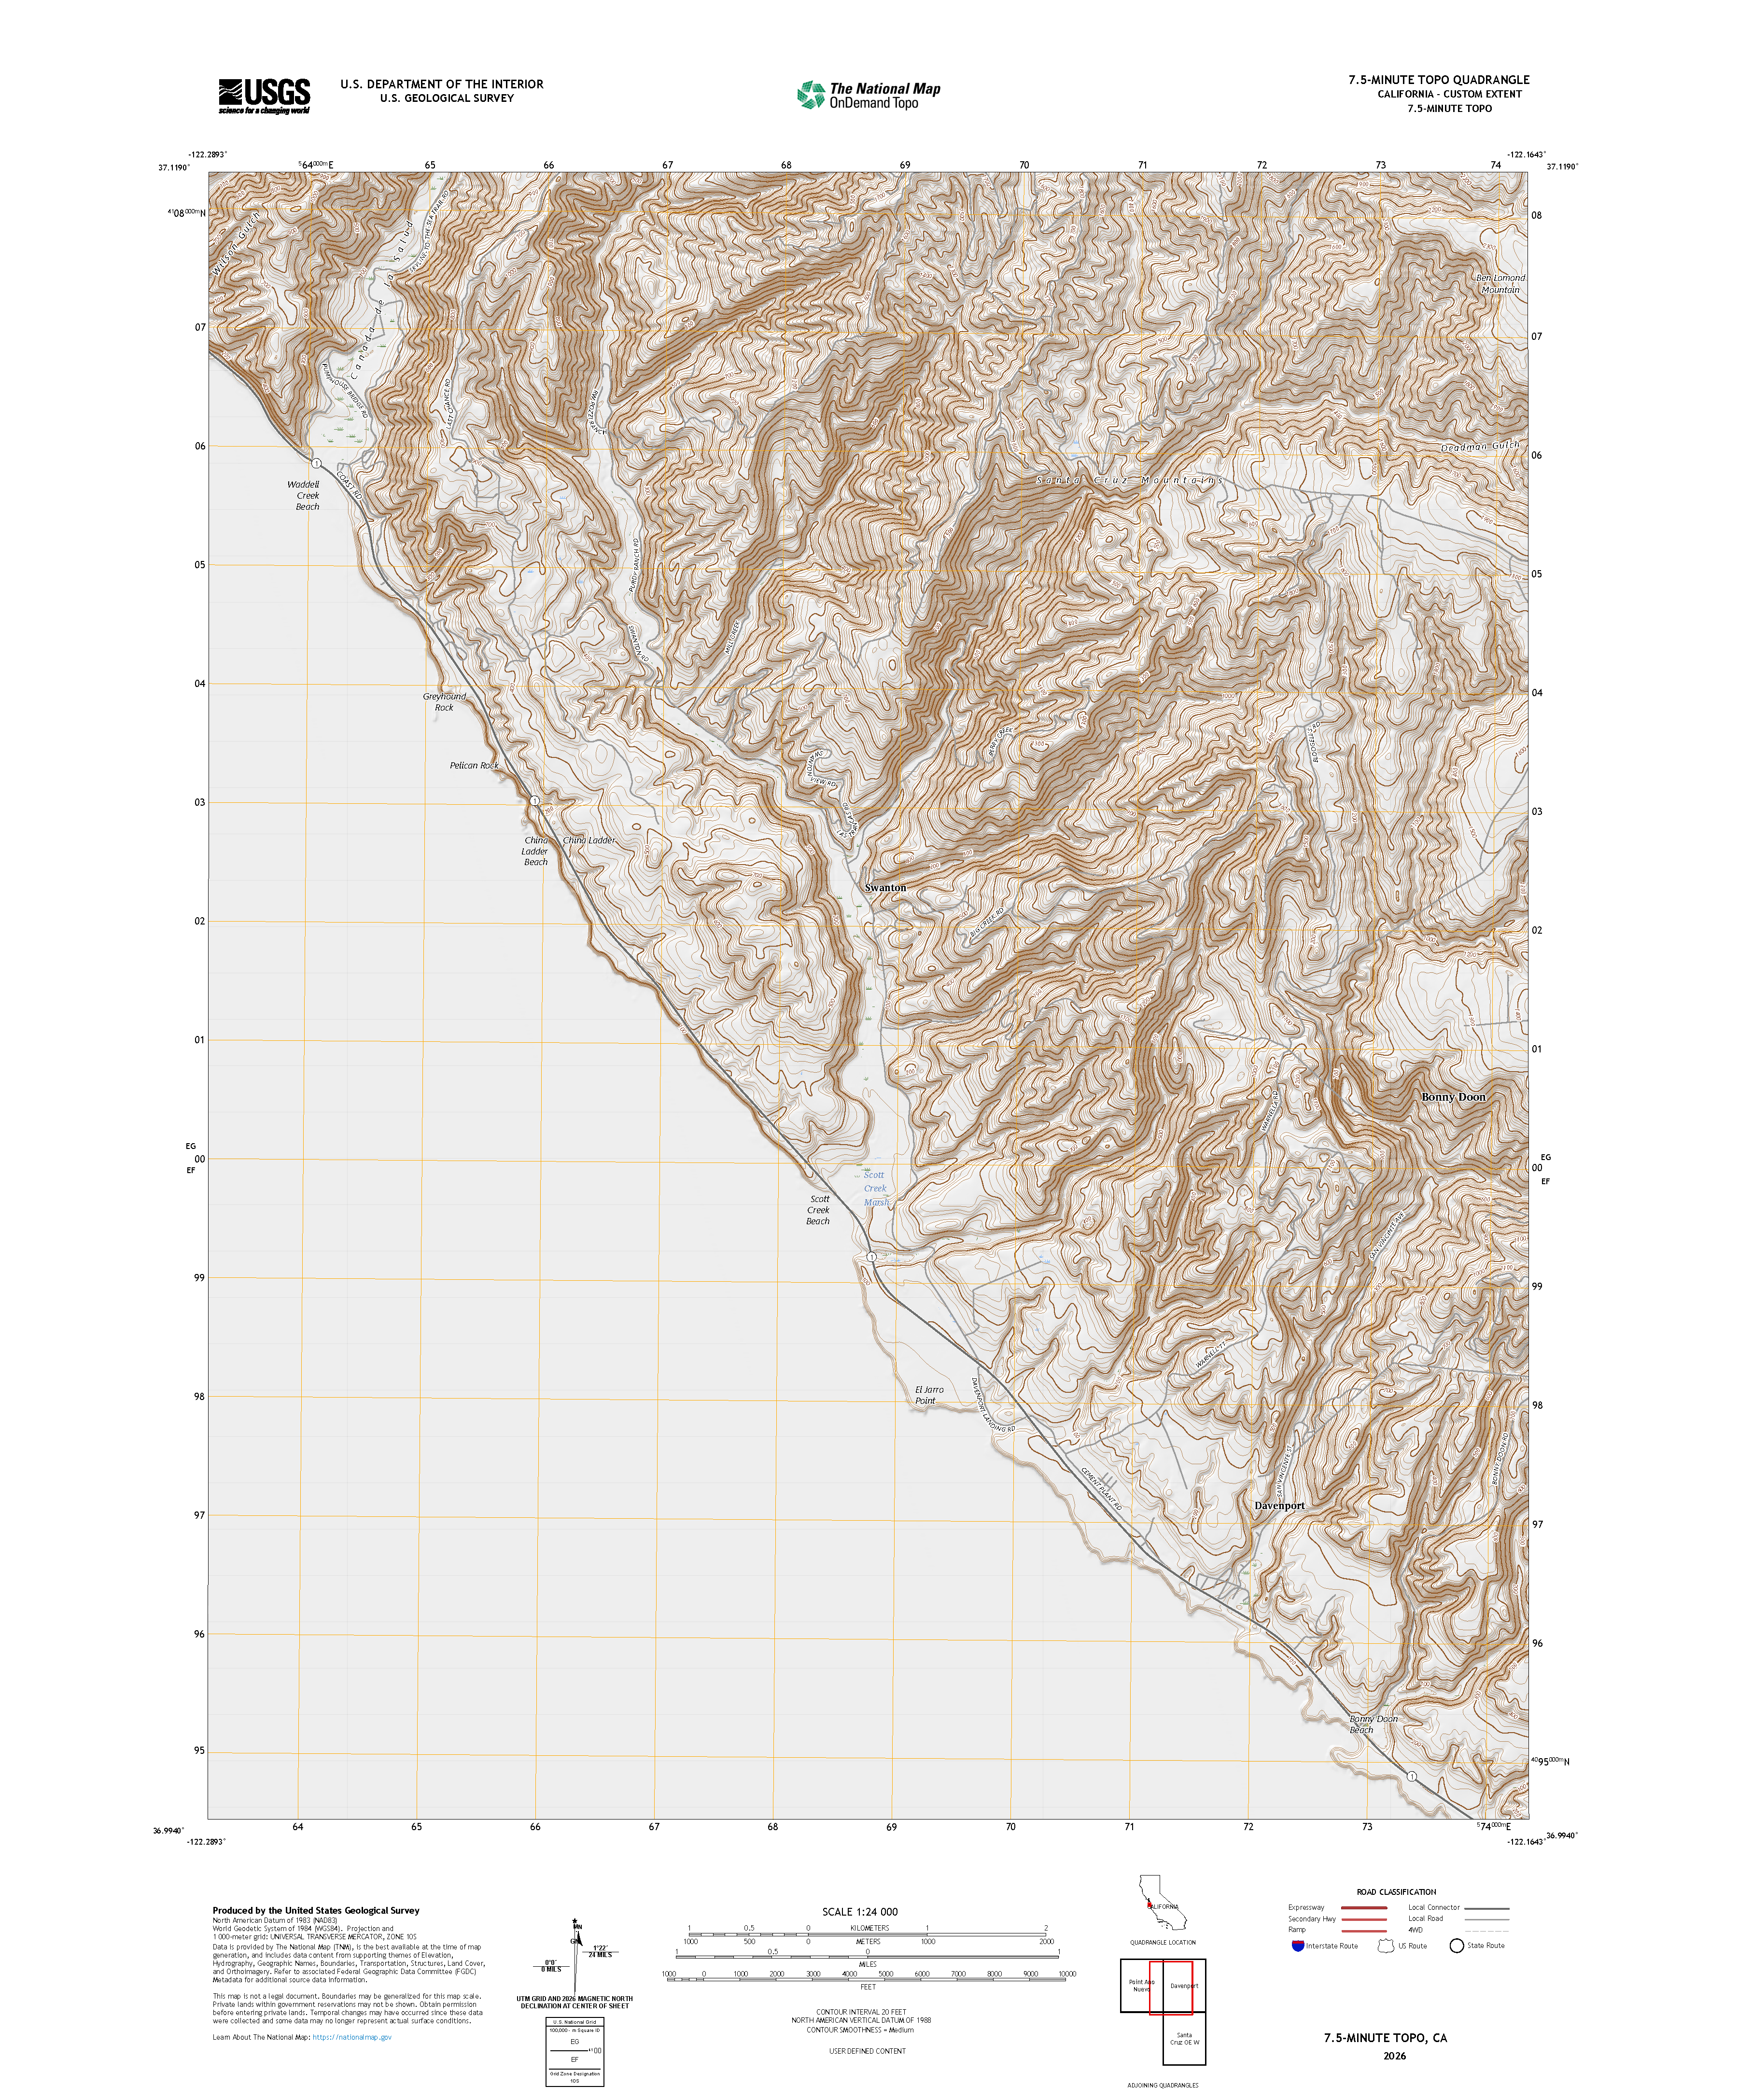
\includegraphics[max width=\linewidth]{Images/CA_75MinuteTopo1_20260611_002516641129_TM_geo.pdf}
    \caption[USGS topographic map, Swanton Ranch area]{USGS 7.5-minute
    topographic map of the Swanton Ranch area at 1:24,000 scale.}
    \label{fig:topo}
\end{figure}

\subsection{Citizens Broadband Radio Service (CBRS)}

The Citizens Broadband Radio Service is a shared-spectrum framework established
by the FCC covering 150~MHz of mid-band spectrum from 3.550 to 3.700~GHz,
designated as LTE Band~48 \autocite{fcc2015cbrs}. The FCC introduced the
framework in 2015 and completed the operational rules by 2020. CBRS represents
a significant departure from the traditional spectrum licensing model, where a
carrier purchases exclusive rights to a band through a government auction and
deploys a network at its own discretion. Instead, CBRS uses a dynamic spectrum
sharing architecture that allows multiple users to share the same frequencies
under managed coexistence rules.

The sharing framework operates through a three-tier hierarchy, illustrated in
Figure~\ref{fig:cbrs_tiers} \autocite{fcc2015cbrs}:

\textbf{Tier 1: Incumbents.} The highest-priority users are existing incumbent
licensees, primarily US Navy radar systems and satellite earth stations. When
Tier~1 systems are detected or operating in an area, all lower-tier users in
that area must immediately cease operation. No notice is provided; the cessation
is automatic and mandatory. At Swanton Ranch, which sits on the Pacific coast,
this tier represents a meaningful operational consideration. US Navy vessels
operating offshore could trigger preemption events with no warning.

\textbf{Tier 2: Priority Access Licenses (PAL).} The second tier consists of
organizations that have purchased licensed access to a specific 10~MHz channel
within CBRS in a defined geographic area through an FCC auction. PAL holders
receive protection from other PAL users and from Tier~3 users. PAL licenses are
available for county-sized geographic areas and represent a way to secure
predictable spectrum access for a long-term deployment.

\textbf{Tier 3: General Authorized Access (GAA).} The third tier is open to all
users without any license or registration fee. GAA users may operate on any
CBRS frequency that is not already occupied by Tier~1 or Tier~2 users, but they
receive no protection from interference by other Tier~3 users or from PAL
holders, and they must yield immediately if a higher-tier user appears. The
network deployed in this project operates at Tier~3, GAA access.

The mechanism enforcing these tiers is the Spectrum Access System (SAS). Every
CBRS device must register with an SAS and receive a channel grant before it can
transmit. The SAS tracks the locations of all registered devices, the locations
and operating schedules of incumbent systems, and the PAL license geography, and
it dynamically allocates available channels to GAA users. For outdoor operation,
CBRS devices must be registered by a Certified Professional Installer (CPI) and
must communicate their precise GPS location to the SAS. For the Swanton
deployment, the radio was configured in a non-SAS ``Other'' mode appropriate for
field-testing outside of normal public radiation rules. A permanent installation
would require full SAS registration and CPI certification, as discussed in
Section~VIII.C.

CBRS is particularly well suited to the Swanton use case for several reasons. It
operates at 3.5~GHz, a mid-band frequency that provides a useful balance between
coverage range and throughput capacity. It is compatible with standard commercial
smartphones and LTE user equipment, meaning ranch staff and students can use
ordinary phones without any special hardware. The spectrum is available at no
licensing cost for GAA access, which fits the project's budget constraints. And
the ecosystem of compliant hardware, including the Baicells radio used in this
project, is well-developed and commercially available at price points that make
private deployment economically viable.

\begin{figure}[!ht]
    \centering
    \fbox{%
        \parbox[c][2.5in][c]{0.90\linewidth}{%
            \centering
            \textbf{CBRS Three-Tier Spectrum Access Framework}\par
            \vspace{0.5em}
            \textit{Replace with CBRS three-tier framework diagram.}%
        }%
    }
    \caption[CBRS three-tier spectrum access framework]{CBRS three-tier
    spectrum access framework: Incumbents (Tier~1), Priority Access Licenses
    (Tier~2), and General Authorized Access (Tier~3).}
    \label{fig:cbrs_tiers}
\end{figure}

\subsection{CBRS Spectrum Policy Context}

The framework that makes this project possible is not static. The FCC is
actively considering changes to the CBRS band, including proposals that would
allow higher power levels and potentially relocate existing users to accommodate
larger commercial deployments \autocite{lupo2026cbrs}. These proposals reflect
pressure from major carriers seeking to expand their mid-band holdings, and they
would have significant consequences for the class of deployments this project
represents.

Higher transmit power in CBRS would increase interference across the band,
degrading the reliability of existing small-scale networks. If power levels are
raised to accommodate carrier-scale operations, the low-power private
deployments at universities, industrial facilities, and rural sites like Swanton
Ranch would face degraded signal-to-interference ratios. In practical terms, the
same network infrastructure built in this project would deliver measurably worse
performance in a higher-power CBRS environment.

Cal Poly has a direct institutional stake in how these policy questions are
resolved. The Avila Beach marine research pier, the Digital Transformation Hub
on the main campus, and the Swanton Ranch network all depend on the current CBRS
framework. In May 2026, Christopher Lupo, Founding Director of the Noyce School
of Applied Computing at Cal Poly, published an article in \textit{RCR Wireless},
one of the major national RF and telecommunications trade publications, arguing
against the proposed changes \autocite{lupo2026cbrs}. The article,
co-developed with the Cal Poly 5G Innovation Lab, described Cal Poly's CBRS
deployments and their educational and research value. It received approval from
the Chancellor's office before publication, reflecting the institutional
significance of the issue.

The argument in that article applies directly here: none of the work described
in this report is possible without the spectrum policy framework that CBRS
provides. The technical choices made at every layer of this project---the
frequency band, the hardware, the power levels, the simulation
assumptions---all flow from the assumption that shared CBRS spectrum remains
accessible to non-carrier users.

\subsection{LTE Technical Background}

LTE (Long-Term Evolution) is the fourth-generation cellular standard developed
by the 3rd Generation Partnership Project (3GPP). Understanding the key
architectural components and air interface concepts is necessary to follow the
design and implementation decisions in this report.

\textbf{Network Architecture}

An LTE network consists of two major subsystems: the Radio Access Network (RAN)
and the Evolved Packet Core (EPC). The RAN is composed of eNodeBs (evolved
Node~Bs), the base stations that communicate directly with user equipment over
the radio interface. In this project, the Baicells Nova 846 is the eNodeB. The
EPC handles authentication, mobility management, session management, and data
routing. It is composed of several interconnected network
functions \autocite{hpe2019cbrsradio,hpe2019cbrssignaling}:

\begin{itemize}
    \item \textbf{MME (Mobility Management Entity):} Handles User Equipment
    (UE) authentication, mobility state management, and session establishment.
    The MME communicates with the eNodeB over the S1-MME interface using the
    S1AP protocol over SCTP. In this project, the MME runs as part of Open5GS
    on the Intel NUC at IP address 10.0.1.4.

    \item \textbf{HSS (Home Subscriber Server):} The subscriber database. It
    stores the authentication credentials (IMSI, Ki, OPc) and subscriber
    profiles for every device authorized on the network. The HSS is also part
    of the Open5GS stack in this project.

    \item \textbf{SGW (Serving Gateway) and PGW (PDN Gateway):} Together these
    form the user-plane data path. The SGW anchors the user-plane connection to
    the eNodeB, while the PGW connects to external data networks, in this case
    the internet via Starlink. In this project, the data plane was handled by
    Baicells LGW (Local Gateway) NAT mode, as discussed in Section~VII.E.
\end{itemize}

\textbf{LTE Air Interface}

LTE uses Orthogonal Frequency Division Multiplexing (OFDM) for the downlink and
Single-Carrier Frequency Division Multiplexing (SC-FDMA) for the uplink. OFDM
divides the available spectrum into many orthogonal subcarriers, each carrying a
small portion of the data stream. This makes LTE resilient to multipath
propagation, which is particularly relevant in the hilly coastal terrain at
Swanton. The base unit of resource allocation in LTE is the Resource Block (RB),
which occupies 180~kHz of bandwidth and one 0.5~ms slot in time. A 20~MHz LTE
carrier contains 100 resource blocks, and the scheduler at the eNodeB
dynamically allocates resource blocks to connected devices based on signal
quality and traffic demand \autocite{hpe2019cbrsradio}.

CBRS Band~48 uses Time Division Duplexing (TDD), meaning the same frequency is
used for both downlink (base station to UE) and uplink (UE to base station),
with time slots alternating between the two directions. This contrasts with FDD
(Frequency Division Duplexing), which uses separate frequency blocks for uplink
and downlink simultaneously. TDD is well suited to asymmetric traffic loads
because the ratio of downlink to uplink slots is configurable. This project used
TDD SubFrame Assignment~2, which allocates three downlink subframes for every
one uplink subframe, a 3:1 ratio appropriate for a network where users primarily
receive data (web browsing, sensor downlink) rather than upload large quantities
\autocite{houtz2026wlpc}.

\textbf{MIMO}

LTE supports multiple-input multiple-output (MIMO) antenna configurations. The
Nova 846 has eight physical antenna ports and can operate in either 4T4R
(4~transmit, 4~receive) or 8T8R configuration. This project operated in 4T4R
single-carrier mode, connecting four of the eight antenna ports to the
AW3376-E-F sector antenna. MIMO improves both throughput and link reliability by
transmitting multiple independent data streams simultaneously on spatially
separated antenna paths, exploiting the natural multipath propagation in the
radio environment.

\textbf{Signal Quality Metrics}

G-NetTrack Lite, the application used for drive test data collection, logs RSRP
(Reference Signal Received Power) as its primary signal quality metric. RSRP
measures the average power of the LTE reference signals received from the
serving cell, measured in dBm \autocite{hpe2019cbrsradio}. The reference signal
is a known pilot pattern transmitted by the eNodeB, and its received power gives
a clean measure of path loss independent of traffic load. The standard RSRP
quality categories used in this report are shown in Table~\ref{tab:rsrp}.

\begin{table}[!ht]
    \centering
    \caption[RSRP quality classification]{Standard RSRP quality
    classification.}
    \vspace{0.5\baselineskip}
    \begin{tabular}{lc}
        \toprule
        \textbf{RSRP Range} & \textbf{Quality Classification} \\
        \midrule
        $>-80$~dBm       & Strong     \\
        $-80$ to $-90$~dBm   & Good       \\
        $-90$ to $-100$~dBm  & Fair       \\
        $-100$ to $-110$~dBm & Marginal   \\
        $-110$ to $-120$~dBm & Weak       \\
        $-120$ to $-130$~dBm & Very Weak  \\
        \bottomrule
    \end{tabular}
    \label{tab:rsrp}
\end{table}

\textbf{SIM Authentication}

Every device on an LTE network is authenticated through its SIM card using the
Milenage Authentication and Key Agreement (AKA) protocol
\autocite{hpe2019cbrssignaling}. The SIM stores two secret values: the Ki
(authentication key) and the OPc (operator-specific authentication code derived
from a root operator key). When a device attempts to attach to the network, the
MME retrieves the subscriber record from the HSS and runs the AKA protocol. The
protocol performs mutual authentication: the network proves its identity to the
UE, and the UE proves its identity to the network, both using shared secret keys
that are never transmitted over the air. Session encryption keys are derived
fresh at each attachment, so capturing previous sessions provides no information
useful for decrypting future ones. This security architecture is relevant to the
Swanton use case because the ranch network would eventually carry sensitive
research data and potentially safety-critical communications.

\subsection{RF Propagation Simulation and Tool Democratization}

RF propagation simulation allows network designers to model signal coverage
before deploying hardware in the field. For a site like Swanton Ranch, where
terrain complexity makes analytical path loss calculations insufficient and where
sending hardware to the field before having a sense of where to point the
antenna would be wasteful, simulation is a necessary planning step.

The tool used in this project is eino.ai, a cloud-native, GPU-accelerated RF
simulation platform \autocite{einoai2024}. eino.ai uses ray-tracing algorithms
against high-resolution terrain data, including LiDAR elevation models, to
compute RSRP coverage maps across a defined simulation area. The output is a
georeferenced RSRP heatmap that can be exported as a KMZ file and layered over
satellite or topographic base maps in Google Earth.

What makes eino.ai notable in this context is the cost relative to its
predecessors. Ten years ago, ray-tracing RF simulation capable of the fidelity
eino.ai provides required a dedicated workstation running specialized thick-client
software that cost on the order of \$50,000. That kind of tool was available
only to large telecom engineering firms and carriers. Today, eino.ai delivers
equivalent capability through a web browser for approximately \$1,000. The shift
from dedicated workstation to cloud platform, enabled by GPU compute becoming
widely available through cloud providers, has put professional-grade propagation
simulation within reach of a university project.

This cost compression in simulation tools mirrors the cost compression in
hardware and spectrum access described in Section~I.A. The same structural shift
that brought the eNodeB hardware cost from hundreds of thousands of dollars to
thousands, and spectrum access from hundreds of millions to zero, has brought
simulation tools from tens of thousands of dollars to thousands. All three
components are now accessible to the same class of user: an organization with a
small budget, technical staff who understand the tools, and a genuine need for
the capability.

% =============================================================================
\section{Requirements}
% =============================================================================

\subsection{Project Goals and Constraints}

The primary goal of this project was to demonstrate a working private LTE
network at Swanton Pacific Ranch and to document the complete system in
sufficient detail that future student teams can build directly on the work. This
framing deliberately prioritized completeness and documentation over
optimization. A polished but poorly documented deployment would leave the next
group starting over from the beginning.

Several constraints influenced the final design. The deployment site is
accessible only by driving to the ranch, which limits the complexity of hardware
that can be transported and assembled by a small team without heavy equipment.
Power at Cooke's Peak is currently limited to a solar panel supporting the UHF
repeater; additional infrastructure was not available for the initial deployment,
which meant relying on a portable battery bank for power. The budget was
constrained to \$500 for hardware not provided by donors. Standard phone
compatibility was a firm requirement, both for the initial testing and for the
eventual ranch user base; the network needed to work with off-the-shelf Android
and iOS devices without custom firmware or specialized hardware. Finally, the
deployment approach needed to be temporary and reversible, since no structural
modification to the site was authorized for this initial phase.

\subsection{Marketing Requirements}

The marketing requirements describe what the network needs to provide from the
perspective of end users and ranch stakeholders. They were developed through
conversations with the ranch management and the project advisors, and refined
against the technical constraints.

The top-level requirements are: reliable connectivity, sufficient throughput for
data and video applications, adequate geographic coverage across the working
areas of the ranch, low enough power draw to be sustained by solar
infrastructure, environmental durability appropriate for an outdoor coastal
installation, and minimal visual and physical impact on the ranch environment.

Figure~\ref{fig:mktreq} shows the marketing requirements hierarchy tree.
Table~\ref{tab:pairwise} shows the pairwise weighting used to derive relative
priorities.

\begin{figure}[!ht]
    \centering
    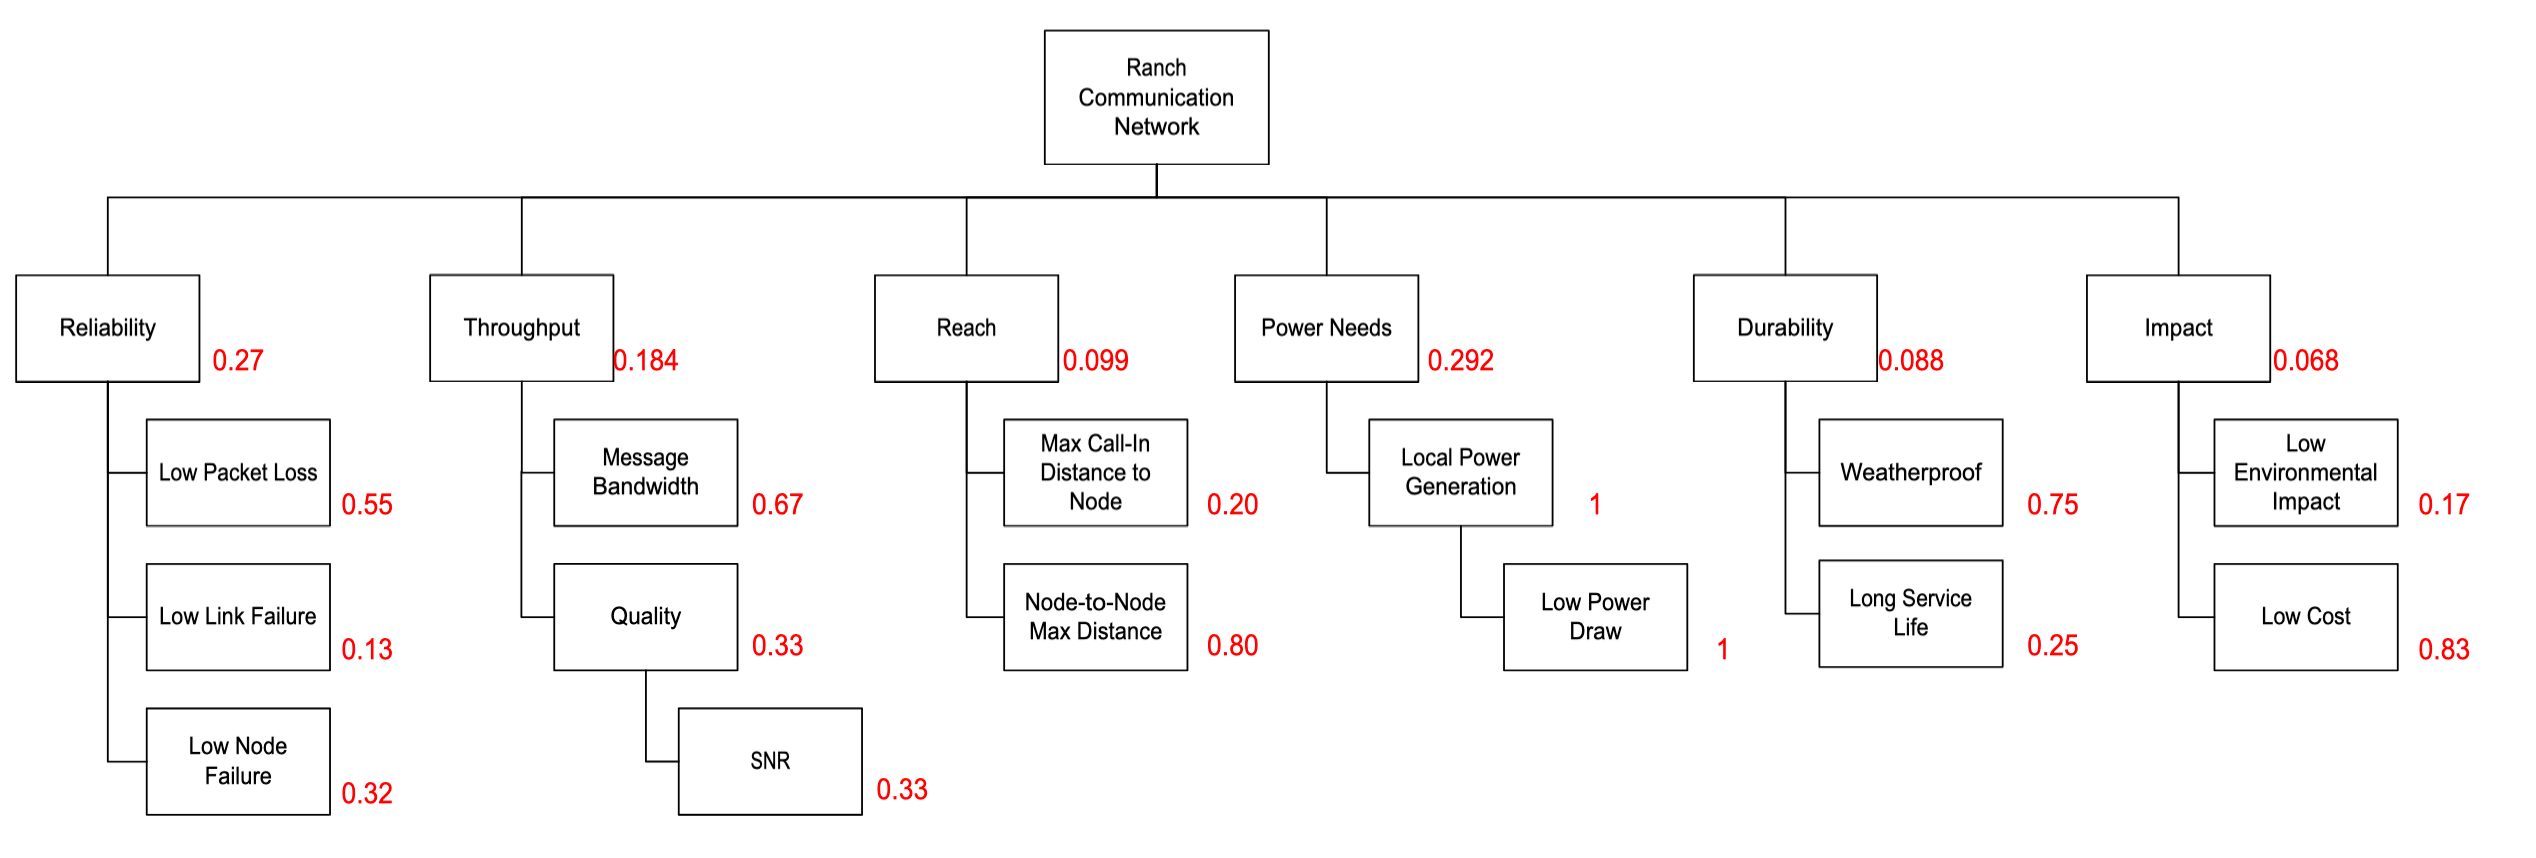
\includegraphics[max width=\linewidth]{Images/Marketing Requirements Hierarchy Tree.png}
    \caption[Marketing requirements hierarchy tree]{Marketing requirements
    hierarchy tree showing top-level requirements and their sub-requirements.}
    \label{fig:mktreq}
\end{figure}

\begin{table}[!ht]
    \centering
    \caption[Pairwise marketing requirements weighting]{Pairwise marketing
    requirements weighting.}
    \vspace{0.5\baselineskip}
    \resizebox{\linewidth}{!}{%
    \begin{tabular}{lccccccr}
        \toprule
        \textbf{Requirement} & \textbf{Reliability} & \textbf{Throughput}
            & \textbf{Coverage} & \textbf{Power} & \textbf{Durability}
            & \textbf{Impact} & \textbf{Weight} \\
        \midrule
        Reliability  & ---  & 3.0 & 3.0 & 0.5 & 2.0 & 5.0 & 0.270 \\
        Throughput   & 0.3  & --- & 3.0 & 0.5 & 3.0 & 3.0 & 0.184 \\
        Coverage     & 0.3  & 0.3 & --- & 0.5 & 1.0 & 2.0 & 0.099 \\
        Power        & 2.0  & 2.0 & 2.0 & --- & 3.0 & 3.0 & 0.292 \\
        Durability   & 0.5  & 0.3 & 1.0 & 0.3 & --- & 1.0 & 0.088 \\
        Impact       & 0.2  & 0.2 & 0.5 & 0.3 & 1.0 & --- & 0.068 \\
        \bottomrule
    \end{tabular}%
    }
    \label{tab:pairwise}
\end{table}

\noindent\textit{Note: A value of 1 means the row requirement has the same
weight as the column requirement in pairwise comparison. Weight is the relative
weight of each need compared to all others.}

\subsection{Engineering Specifications}

The engineering specifications translate the marketing requirements into
measurable targets. They were derived from the marketing requirements hierarchy
and from the technical literature on private LTE performance.

\begin{table}[!htbp]
    \centering
    \caption[Engineering specifications]{Engineering specifications.}
    \vspace{0.5\baselineskip}
    \begin{singlespace}
    \begin{tabularx}{\linewidth}{p{0.30\linewidth}p{0.22\linewidth}X}
        \toprule
        \textbf{Specification} & \textbf{Target} & \textbf{Basis} \\
        \midrule
        Packet loss & $<2\%$ & Data integrity for sensor applications \\
        \addlinespace
        Link uptime & $>99.999\%$ & 5-minute/year downtime ceiling \\
        \addlinespace
        Download throughput & $>10$~Mbps & Supports HD video and concurrent data \\
        \addlinespace
        Signal-to-noise ratio & $>30$~dB & Clean signal for maximum MCS utilization \\
        \addlinespace
        Coverage radius & $>1$~km from deployment site & Ranch working area access \\
        \addlinespace
        End-node power draw & $<100$~W per IoT node & Solar operable without large battery \\
        \addlinespace
        Weatherproofing (radio) & IP65 minimum & Coastal salt air, rain, fog \\
        \addlinespace
        Service life & $>10$ years & Permanent installation durability \\
        \addlinespace
        Environmental impact & No permanent structure for initial deployment & Ranch land use compatibility \\
        \addlinespace
        Total system cost & $<\$500$ for non-donated equipment & University project budget \\
        \bottomrule
    \end{tabularx}
    \end{singlespace}
    \label{tab:engspec}
\end{table}

% =============================================================================
\section{Design}
% =============================================================================

\subsection{Alternatives Analysis}

The team evaluated three fundamentally different architectural approaches for
implementing private cellular connectivity at Swanton Ranch. The central
question in each case was the same: where do the network functions live? The
answer to that question determines the system's behavior under failure
conditions, its cost structure, its security profile, and its long-term
maintainability.

\textbf{Option 1: Fully Integrated All-in-One (HaloB)}

The simplest possible architecture is one where all network functions are
embedded directly in the radio hardware. Baicells offers a product called
HaloB, a ``Lite EPC'' that runs inside the eNodeB itself as a licensed add-on,
available for approximately \$250 \autocite{houtz2025halo}. With HaloB enabled,
the radio handles authentication, session management, and subscriber management
internally. No external core server is required. A phone connects to the
HaloB-equipped radio and can communicate locally without any additional
infrastructure.

The appeal is obvious: fewer components, simpler configuration, faster initial
deployment. For a test setup in a controlled environment, HaloB is a reasonable
choice.

The team rejected HaloB for two reasons. First, HaloB locks the network to
Baicells hardware indefinitely. The subscriber database, authentication
credentials, and network configuration all live inside the eNodeB. If the radio
needs to be replaced or the project migrates to different hardware in the future,
none of that configuration can be migrated. Second, while HaloB does provide
some diagnostic visibility, its configurability is significantly more limited
than a dedicated open-source core. The subscriber management interface,
authentication configuration, and network policy options are all constrained by
what Baicells chose to expose. For a project where understanding every layer of
the stack is part of the educational goal, a core where the team cannot inspect
and modify the underlying network functions misses an important part of the
point.

\textbf{Option 2: Cloud-Hosted Core}

The second option is to run the EPC as a managed cloud service. Several vendors,
including Celona, Highway~9, and GXC Onyx, offer cloud-hosted LTE cores as
subscription services \autocite{houtz2026wlpc}. In this model, the eNodeB at
Swanton connects to a cloud-hosted MME, HSS, and PGW over the internet. The
radio hardware is physically local, but all network intelligence lives in a
remote data center.

The cloud model has real advantages for organizations without the infrastructure
to run and maintain their own servers. Management is outsourced, software updates
are automatic, and scaling is straightforward.

At Swanton Ranch, it fails on a single critical constraint: internet reliability.
The only available internet backhaul at Cooke's Peak is Starlink. While Starlink
is generally reliable, it experiences interruptions due to satellite geometry,
weather, and dish outages. If the Starlink connection goes down, a cloud-dependent
core leaves the ranch with no cellular service at all, including local voice and
data between people who are physically present on the property. The primary use
case for this network includes emergency communication during ranch operations. A
dependency on maintained internet connectivity for all core functions is
incompatible with that requirement.

Additionally, cloud-hosted cores carry recurring subscription costs, typically
billed per radio per month. A 20-year network at a university field site needs a
cost model that does not require ongoing vendor payments.

\textbf{Option 3: Local Open-Source Core (Chosen)}

The chosen approach runs the EPC locally on hardware at the deployment site.
Open5GS is a fully featured open-source LTE and 5G SA core network, licensed
under the AGPL, with an active development community and production deployments
including actual carriers in remote regions
\autocite{waveriders2025open5g2go,houtz2026wlpc}. Open5G2GO is a Docker-based
installer and web UI built by Waveriders Collective that wraps Open5GS with a
one-command installer, a subscriber management interface, and a sensible default
configuration for CBRS PLMN 315-010 \autocite{waveriders2025open5g2go}.

With this architecture, the eNodeB at Swanton connects to an Intel NUC running
Open5GS on the same local LAN. The NUC handles all authentication, session
management, and subscriber database functions independently of the internet.
Users can register on the network, authenticate, and communicate locally even if
Starlink is completely offline. The Starlink connection is used only for routing
UE data traffic to the internet.

The advantages are substantial. The network is self-contained and
internet-independent for its core functions. The software is free and open
source. Every layer of the stack is visible and configurable, which serves the
educational purpose of the project. The documentation burden is manageable, as
Open5G2GO's web UI provides subscriber management without requiring detailed
knowledge of the Open5GS internals. And the team retains complete control over
authentication credentials, security configuration, and network policy.

The main cost is complexity. Setting up Ubuntu Server, Docker, and Open5G2GO on
an Intel NUC, connecting it to a Baicells radio, and troubleshooting the data
path requires Linux and networking familiarity that not all future teams will
have. This report addresses that cost by documenting every step of the process
in detail.

\textbf{Other Technologies Evaluated}

Several other wireless technologies were considered and set aside at the start of
the project:

LoRaWAN provides very long range at very low data rates, suitable for periodic
sensor readings but not for video, voice, or general-purpose data. Its bandwidth
is orders of magnitude below what the ranch needs. LoRaWAN remains interesting
as a secondary backup layer for low-data-rate sensors during CBRS preemption
events, but it cannot serve as the primary connectivity solution.

Wi-Fi HaLow (802.11ah) offers longer range than standard Wi-Fi at sub-GHz
frequencies. During the initial research phase, the team considered a mesh
network using 802.11ah access points. The critical limitation is device
compatibility: standard smartphones and IoT devices do not include 802.11ah
hardware. Every device on the network would require custom hardware, eliminating
the ``standard phones work'' requirement.

AREDN mesh networking operates in amateur radio bands and provides flexible
ad-hoc connectivity, but it requires all operators to hold amateur radio licenses
and prohibits encryption of user traffic. Both of these constraints are
incompatible with a network intended for use by general ranch staff and students.

Fiber reinstallation was considered and dismissed. Restoring the buried fiber
connection destroyed in 2020 would be prohibitively expensive, require months of
construction, and have significant environmental impact on a property still
recovering from a major fire.

\subsection{System Architecture}

Figure~\ref{fig:sysarch} shows the complete system block diagram.

\begin{figure}[!ht]
    \centering
    \fbox{%
        \parbox[c][2.5in][c]{0.90\linewidth}{%
            \centering
            \textbf{System Architecture Block Diagram}\par
            \vspace{0.5em}
            \textit{Replace with system block diagram.}%
        }%
    }
    \caption[System architecture block diagram]{Complete system architecture
    block diagram showing UE, eNodeB, LAN, core network, and Starlink
    backhaul layers.}
    \label{fig:sysarch}
\end{figure}

The physical topology at Swanton Ranch has five layers. At the user device
layer, Android phones configured with APN profiles and loaded with provisioned
SIM cards connect to the eNodeB over the LTE air interface at 3.655~GHz. At the
radio layer, the Baicells Nova 846 eNodeB receives the LTE uplink from UEs,
processes the radio frames, and communicates with the core network over Ethernet
via the S1 interface. The radio is physically mounted on a portable tripod mast
at Cooke's Peak with the AW3376-E-F sector antenna.

At the LAN layer, the eNodeB connects via Ethernet to a small private router
running the 10.0.1.0/24 subnet. The Intel NUC running Open5GS is also on this
subnet, reachable at 10.0.1.4. The S1AP control connection uses SCTP on
port~36412. The user-plane data path uses Baicells LGW NAT mode, which routes
UE traffic through the eNodeB's built-in network address translation rather than
the Open5GS SGW GTP-U tunnel. This configuration is discussed further in
Section~VII.E.

At the core network layer, Open5GS running on the NUC handles MME
(authentication and mobility), HSS (subscriber database), and the PGW function
for IP address assignment. UEs receive addresses from the 10.48.99.0/24 pool,
with static assignments matching subscriber configuration (PHONE-10 receives
10.48.99.10, and so on). The APN is ``internet,'' which routes UE traffic to the
internet through the Starlink connection on the NUC's WAN interface.

At the backhaul layer, a Starlink terminal at the deployment site provides
internet connectivity for UE data traffic routed through the core.

\subsection{RF Link Budget and Antenna Selection}

The transmit power of the Nova 846 is 10~W per transmit channel. With four
active ports in 4T4R configuration, the total radiated power is 40~W, or
46~dBm \autocite{baicells2023nova846}. This power level is appropriate for an
outdoor macro deployment and falls within the allowed transmit power for GAA
CBRS operation.

The AW3376-E-F is an 8-port beamforming panel antenna covering 3,400 to
3,800~MHz, which spans the full CBRS band and CBRS-adjacent bands
\autocite{alphawireless2022aw3376}. Its key specifications for this deployment
are:

\begin{itemize}
    \item Peak gain: 15.5~dBi (standard broadcast beam)
    \item Azimuth beamwidth: 90~degrees
    \item Polarization: $\pm$45-degree slant linear (crossed dipole)
    \item Compatible bands: 3GPP bands 42, 43, and 48; 5G NR n48 and n78
    \item Port count: 8 (supports 8T8R, used here in 4T4R mode)
\end{itemize}

The antenna was selected from the Lawrence Berkeley National Laboratory donation
and represents hardware well above what the project budget would have permitted
independently. MSRP for the AW3376-E-F is approximately \$1,700.

The 4T4R configuration connects ANT ports 0 through 3 on the Nova 846 to the
four lower ports of the AW3376-E-F. According to the Nova 846 installation
guide, single-carrier mode uses only ANT0 through ANT3, and ANT4 through ANT7
are reserved for Cell~2 in dual-carrier configurations
\autocite{baicells2023nova846}. The remaining four antenna ports were left
unconnected and unpowered, as unloaded transmit ports on an active PA would risk
damaging the power amplifier.

The sector was aimed at 120~degrees azimuth, pointing SSE (south-southeast)
toward the main ranch valley and the coastal corridor where activity is
concentrated. Cooke's Peak provides a natural elevation advantage: at 243~m
above sea level, the radio placement is well above the valley floor, maximizing
line-of-sight coverage area. The antenna was mounted at 15~ft (4.6~m) above
ground on a portable tripod mast.

\subsection{RF Propagation Simulation}

Pre-deployment simulation served two purposes. First, it confirmed that Cooke's
Peak was the right location and that a 120-degree sector heading would illuminate
the ranch valley and coastal corridor as intended. Second, it provided reference
predictions to compare against the field measurements collected on May~2, giving
the team a way to assess simulation accuracy and identify the portions of the
property where additional radios would be needed.

\textbf{Simulation Tool}

The simulation was conducted in eino.ai, using its cloud-based ray-tracing
engine against LiDAR terrain data for the Santa Cruz coast region
\autocite{einoai2024}.

\textbf{Simulation Process}

The simulation was set up in five steps, documented in
Figures~\ref{fig:eino_config_area}--\ref{fig:eino_config_antenna}.

\begin{figure}[!ht]
    \centering
    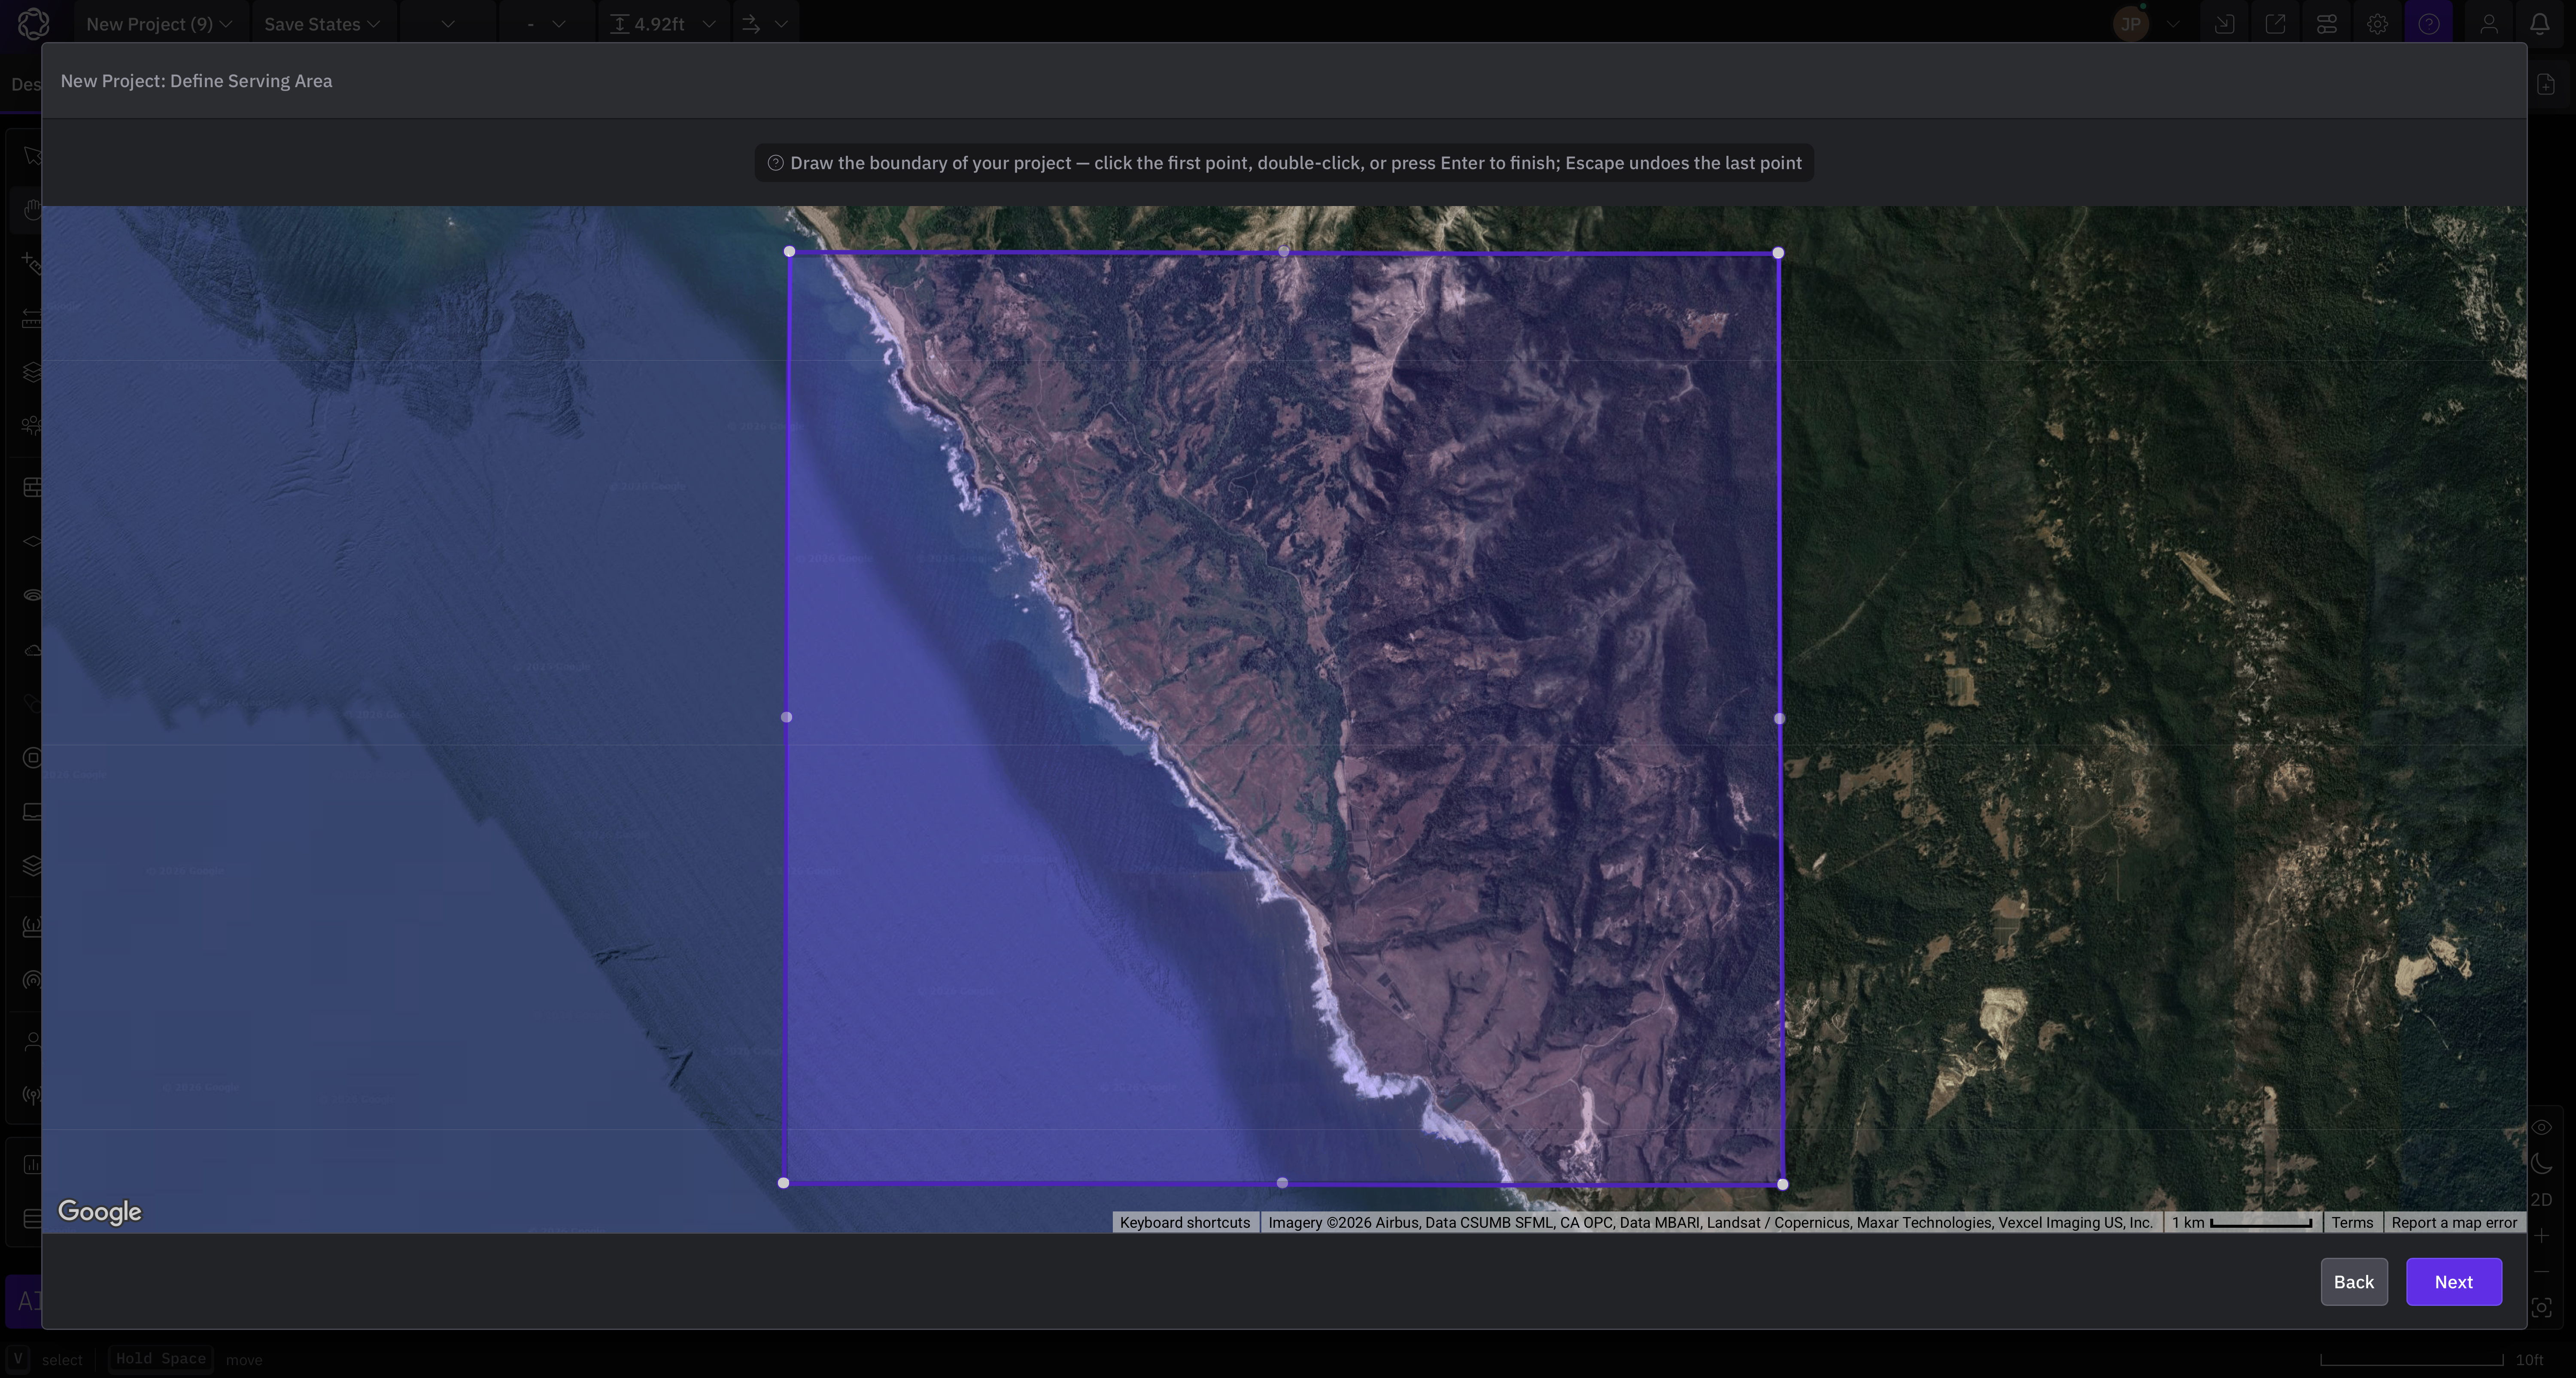
\includegraphics[max width=\linewidth]{Images/Define Simulation area.png}
    \caption[eino.ai simulation area definition]{eino.ai simulation area
    definition: bounding polygon drawn over the Swanton Ranch area.}
    \label{fig:eino_config_area}
\end{figure}

\begin{figure}[!ht]
    \centering
    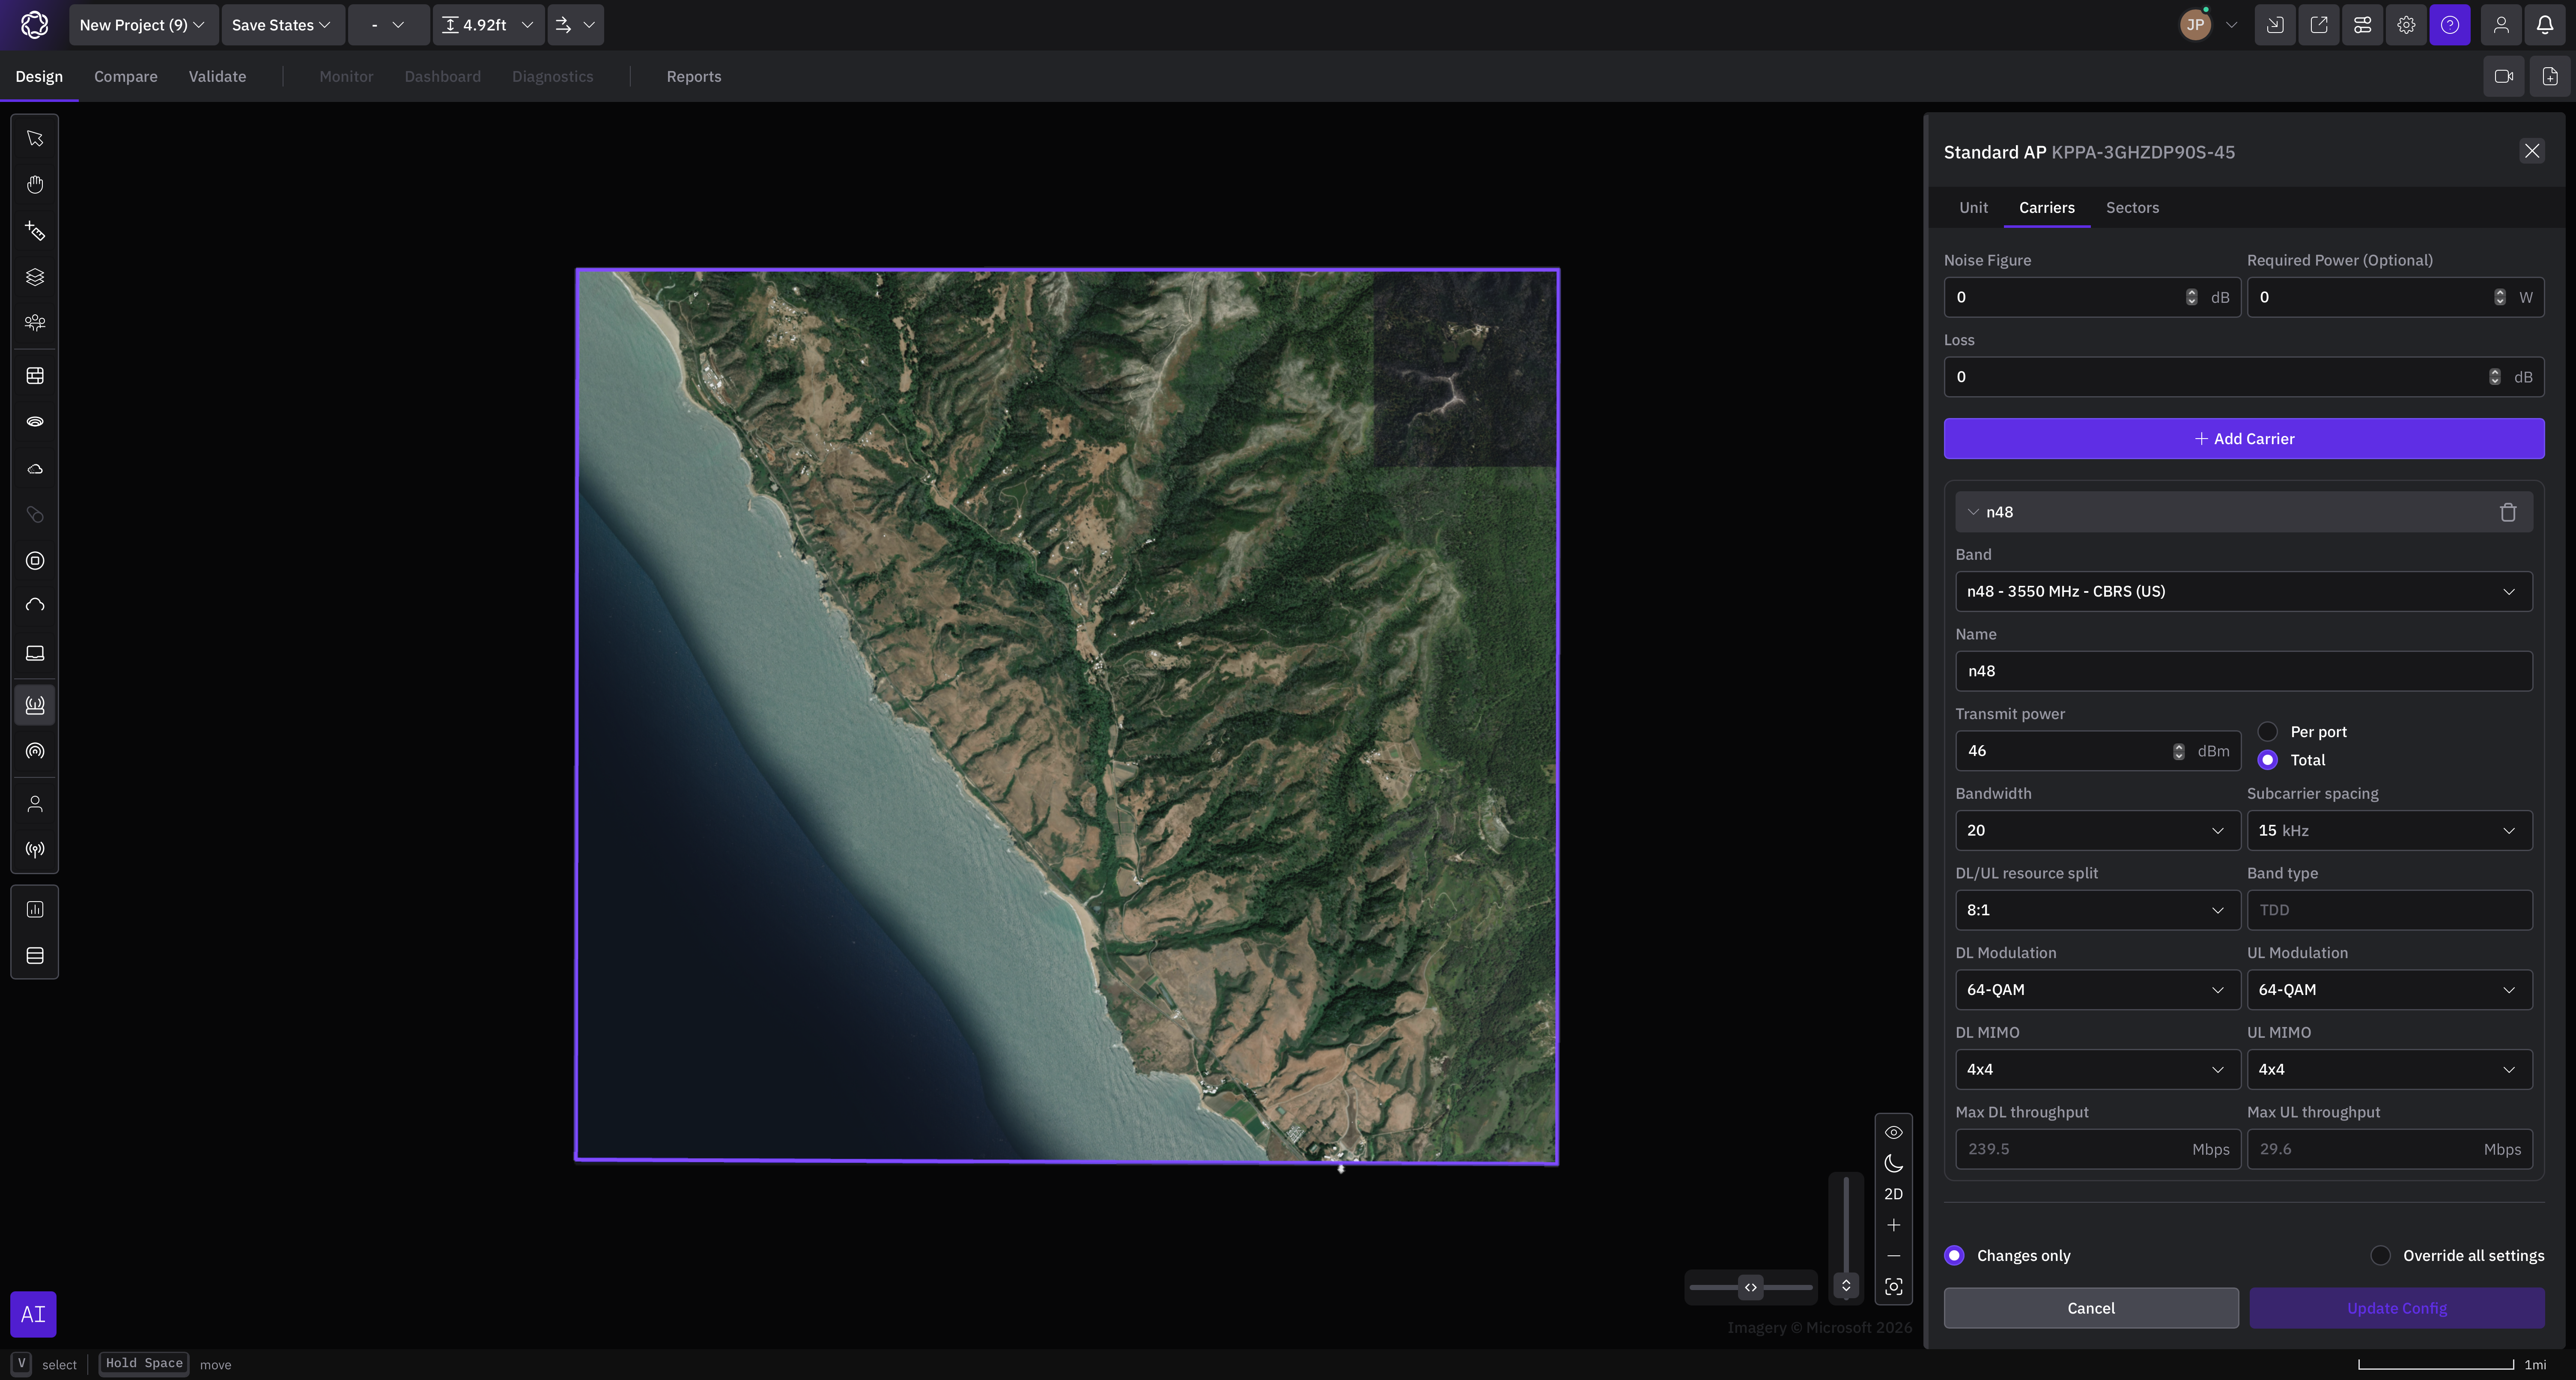
\includegraphics[max width=\linewidth]{Images/Eino AP Carrier Definition.png}
    \caption[eino.ai AP carrier definition]{eino.ai AP carrier definition:
    LTE CBRS Band~48, 20~MHz bandwidth, 4$\times$4 MIMO, 64-QAM.}
    \label{fig:eino_config_carrier}
\end{figure}

\begin{figure}[!ht]
    \centering
    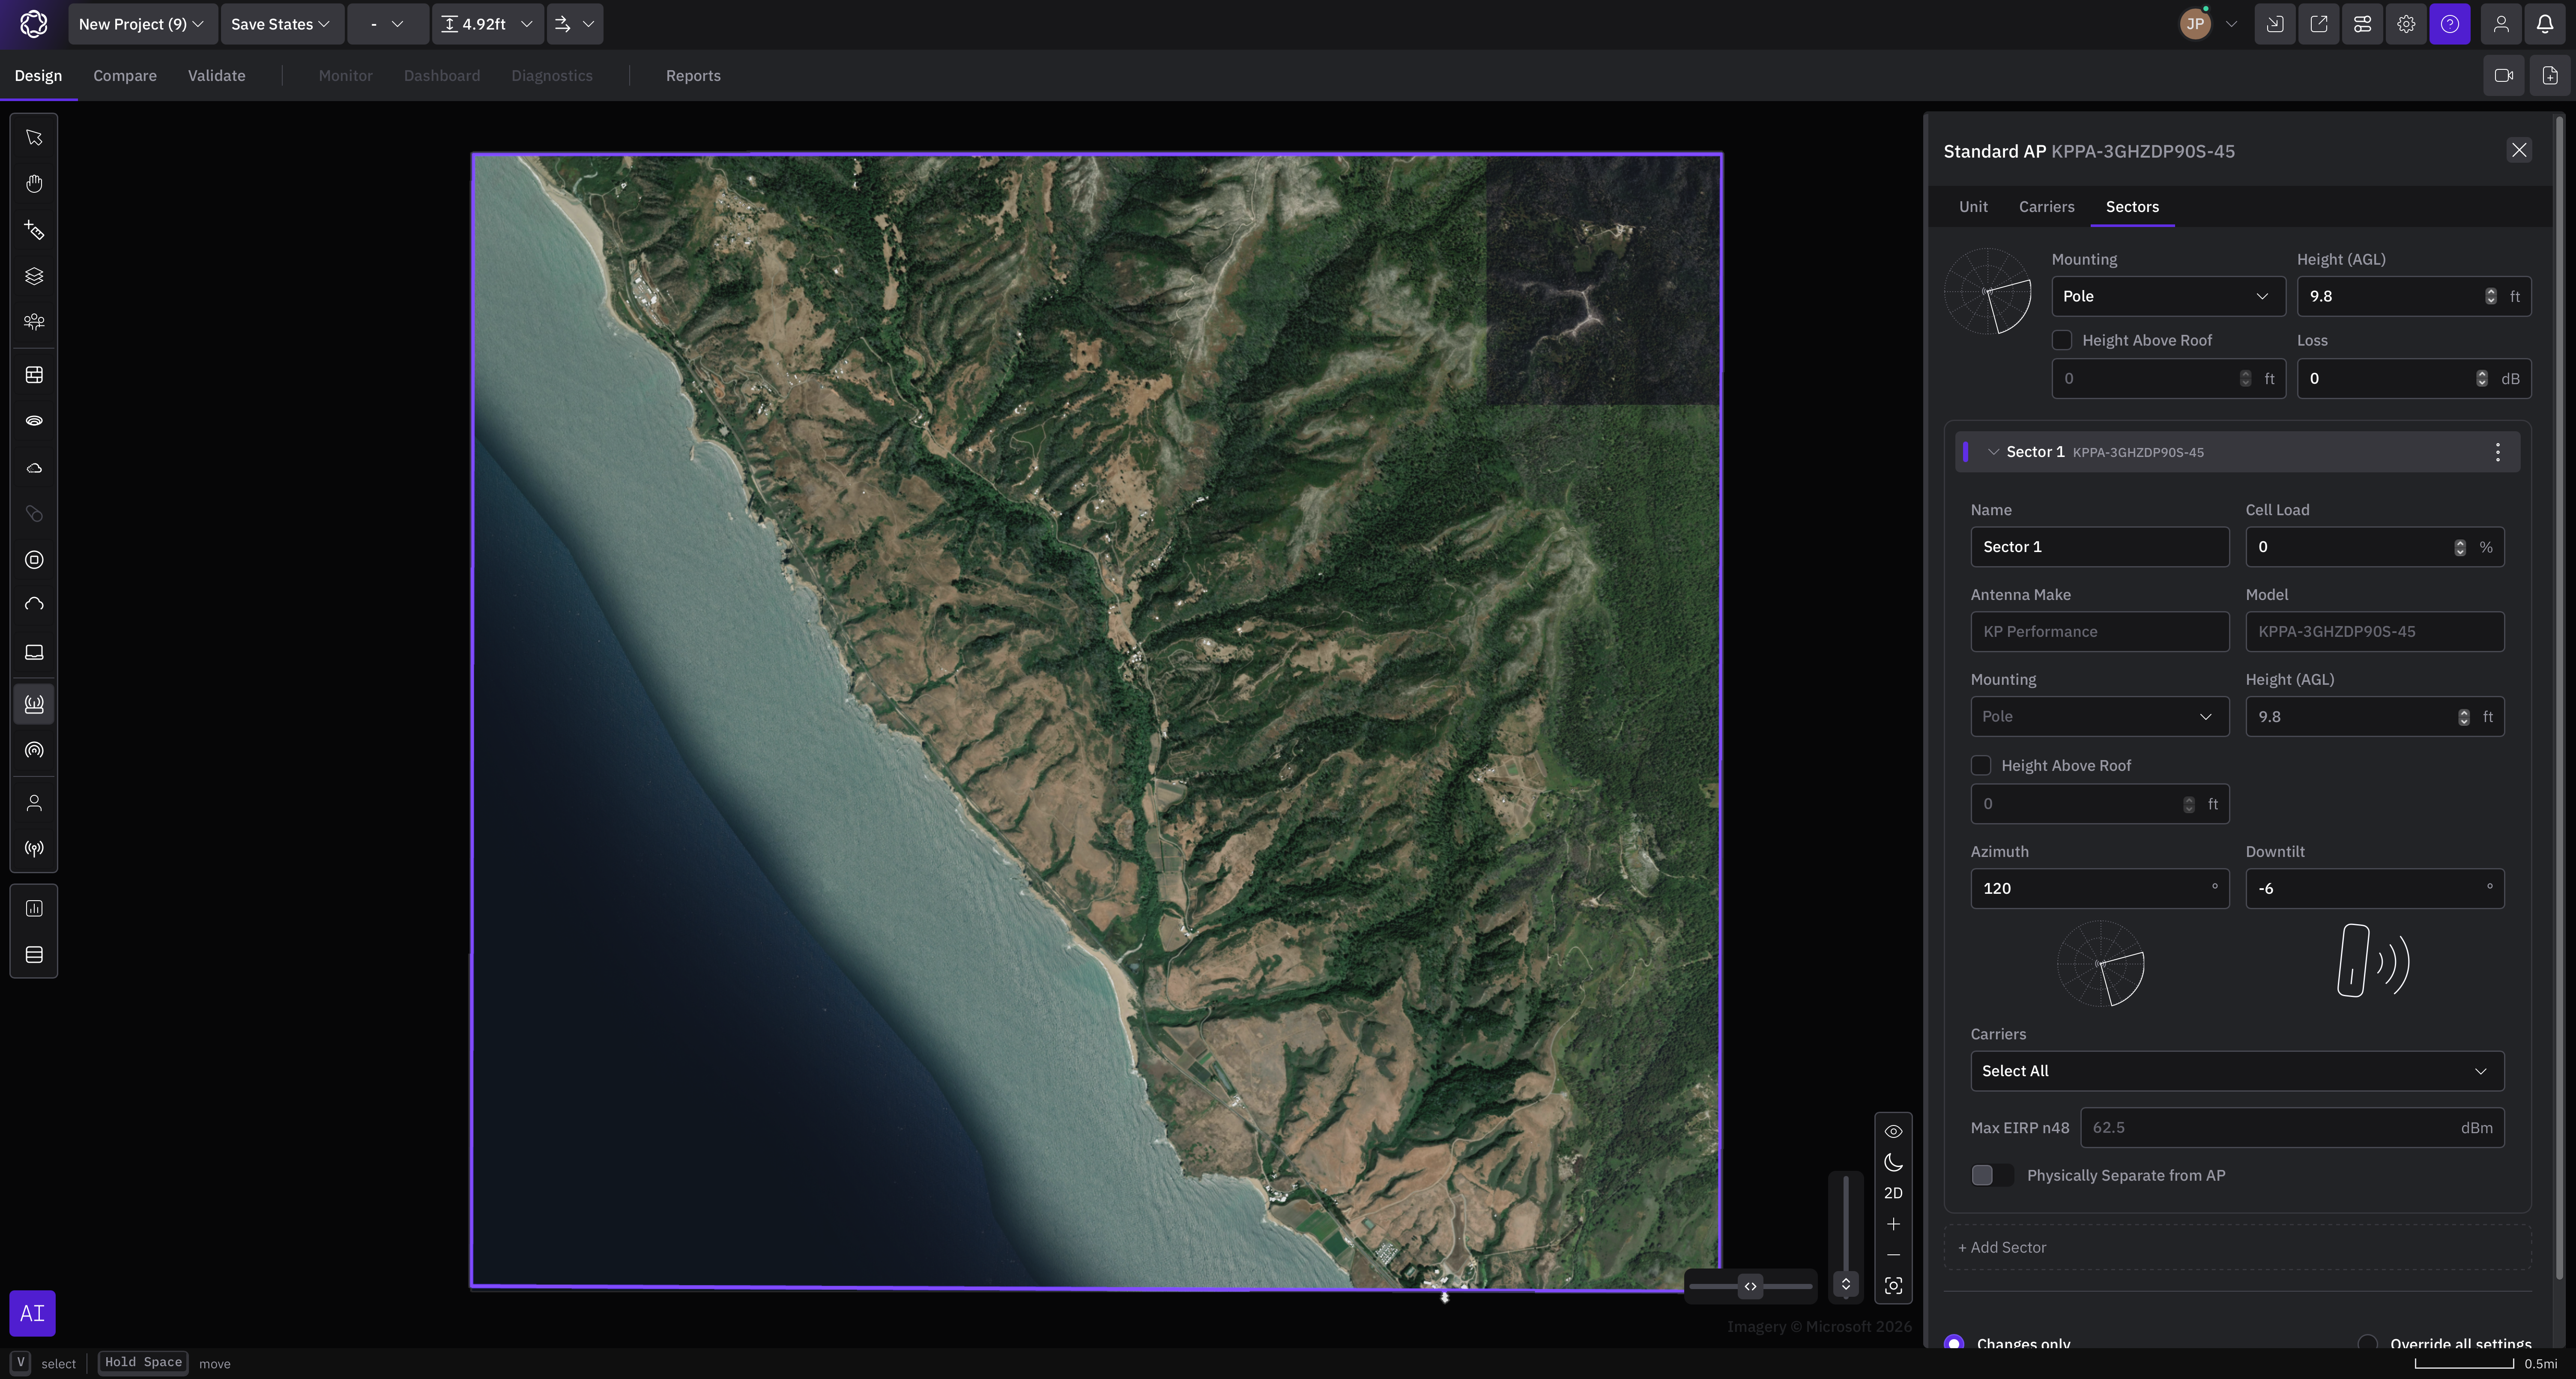
\includegraphics[max width=\linewidth]{Images/Eino AP Sector Definition.png}
    \caption[eino.ai sector definition]{eino.ai sector definition: 120-degree
    azimuth heading, 46~dBm TX power, 4.6~m height above ground.}
    \label{fig:eino_config_sector}
\end{figure}

\begin{figure}[!ht]
    \centering
    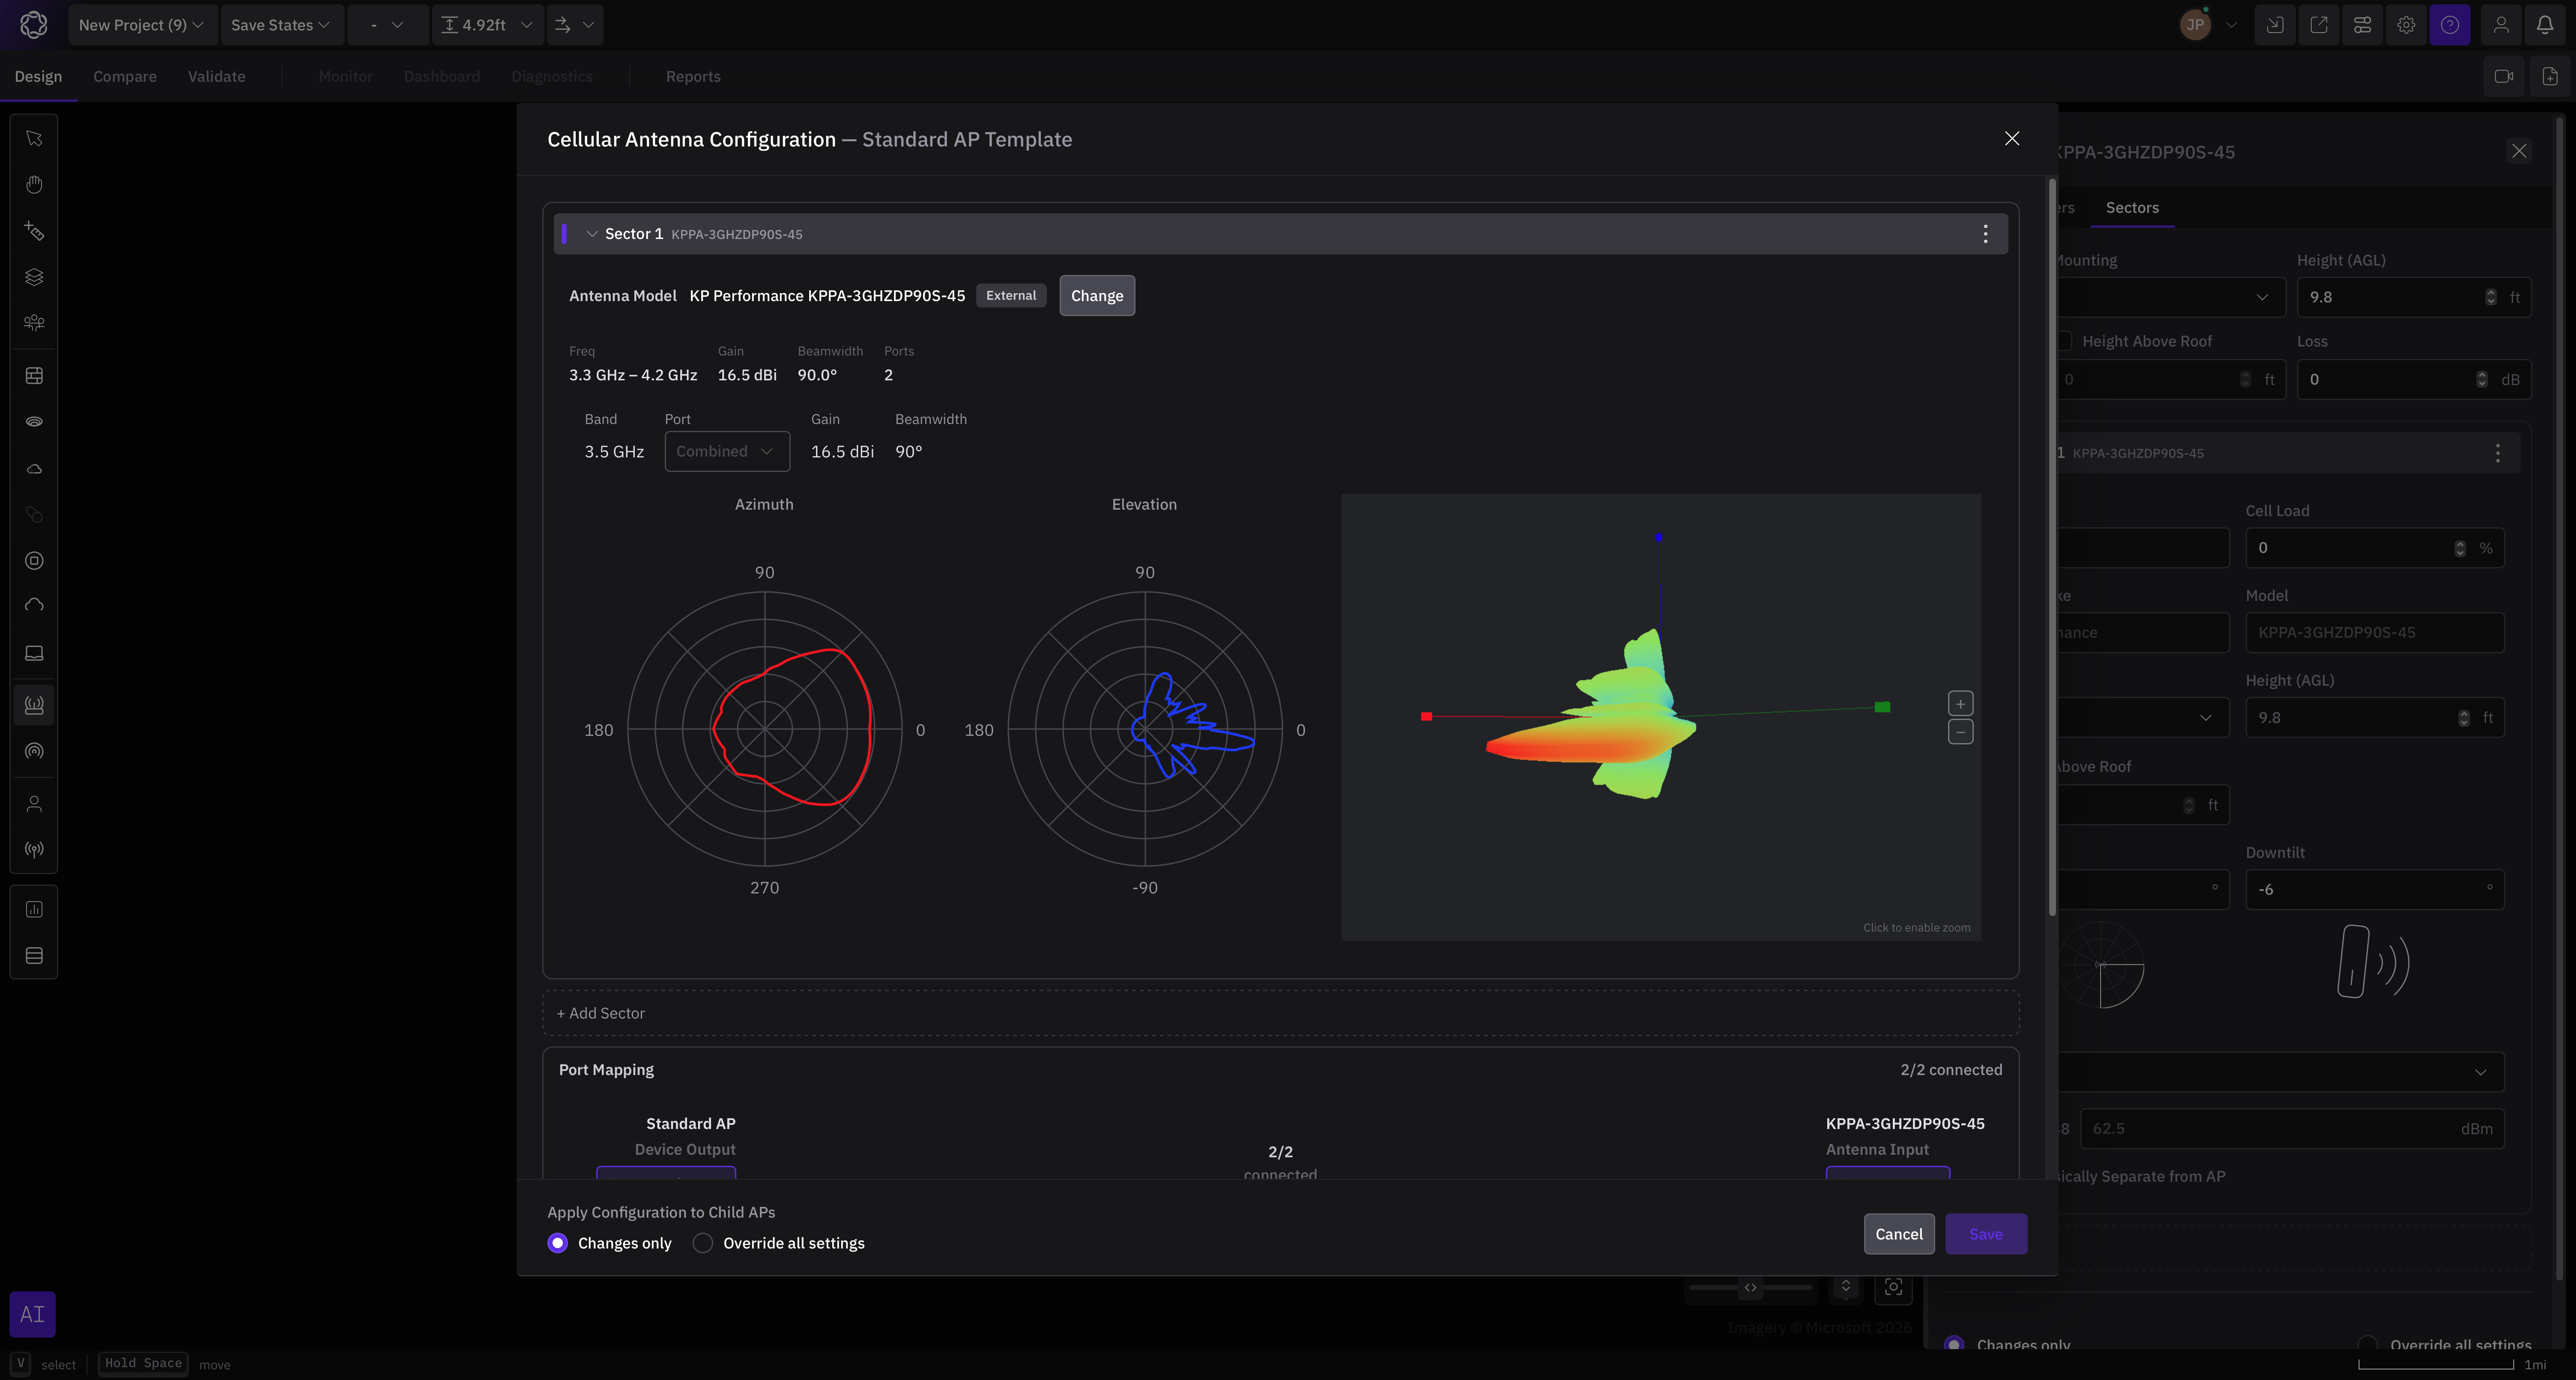
\includegraphics[max width=\linewidth]{Images/Eino Sector Antenna Details.png}
    \caption[eino.ai antenna model selection]{eino.ai antenna model selection:
    KP Performance KPPA-3GHZ0P905-45 used as substitute for the AW3376-E-F.}
    \label{fig:eino_config_antenna}
\end{figure}

First, the simulation area was defined by drawing a bounding polygon over the
Swanton Ranch area in eino.ai's map interface, covering approximately the range
visible from Cooke's Peak and extending south along the coastal corridor.

Second, the access point was placed at Cooke's Peak at coordinates
$-122.2376^{\circ}$ longitude, $37.0650^{\circ}$ latitude, 243~m elevation.
eino.ai uses the actual terrain elevation at the placed point, so the height
above ground parameter represents antenna clearance above the immediate terrain
surface, not elevation above sea level. The antenna was configured at 15~ft
(4.6~m) above the terrain surface at the placement point.

Third, the carrier was configured as LTE CBRS Band~48 (3550~MHz center frequency
in Eino), 20~MHz bandwidth, 4$\times$4 MIMO, 64-QAM modulation.

Fourth, the sector was configured with a 120-degree azimuth heading. The TX
power entered in Eino was 46~dBm, matching the actual deployment transmit power.

Fifth, the antenna model was selected. The AW3376-E-F is not in eino.ai's
antenna library. The closest available model was the KP Performance
KPPA-3GHZ0P905-45, a 90-degree azimuth CBRS sector antenna. The KP Performance
model has a rated gain of 16.5~dBi, compared to the AW3376-E-F's 15.5~dBi. This
1~dB difference makes the simulation marginally optimistic, a systematic
overestimation acknowledged in the results comparison in Section~VII.C.

Table~\ref{tab:simsettings} summarizes the simulation parameters.

\begin{table}[!ht]
    \centering
    \caption[eino.ai simulation parameters]{eino.ai simulation parameters
    compared to actual deployment values.}
    \vspace{0.5\baselineskip}
    \begin{tabular}{p{0.30\linewidth}p{0.30\linewidth}p{0.28\linewidth}}
        \toprule
        \textbf{Parameter} & \textbf{Simulation Value}
            & \textbf{Actual Deployment Value} \\
        \midrule
        Carrier          & LTE, CBRS Band 48 & LTE, CBRS Band 48 \\
        \addlinespace
        Center frequency & 3550~MHz & 3655~MHz (EARFCN 56290) \\
        \addlinespace
        Bandwidth        & 20~MHz & 20~MHz \\
        \addlinespace
        MIMO             & 4$\times$4 & 4T4R \\
        \addlinespace
        Modulation       & 64-QAM & 64-QAM (max) \\
        \addlinespace
        Antenna model    & KP Performance KPPA-3GHZ0P905-45
                         & Alpha Wireless AW3376-E-F \\
        \addlinespace
        Antenna gain     & 16.5~dBi & 15.5~dBi \\
        \addlinespace
        Azimuth beamwidth & 90~degrees & 90~degrees \\
        \addlinespace
        Sector heading   & 120~degrees & 120~degrees \\
        \addlinespace
        AP location      & Cooke's Peak ($-122.2376$, $37.0650$)
                         & Cooke's Peak ($-122.2376$, $37.0650$) \\
        \addlinespace
        TX power         & 46~dBm & 46~dBm total (40~W, 4$\times$10~W) \\
        \addlinespace
        Height above ground & 4.6~m (15~ft) & 4.6~m (15~ft) \\
        \bottomrule
    \end{tabular}
    \label{tab:simsettings}
\end{table}

\textbf{Simulation Results}

The simulation produced the RSRP heatmap shown in Figure~\ref{fig:eino_heatmap}.
The RSRP color scale used by eino.ai assigns green to signals above $-60$~dBm,
yellow-green to $-70$~dBm, yellow to $-80$~dBm, orange to $-90$~dBm, and red
to $-100$ through $-110$~dBm, with areas below this threshold receiving no color
(effectively outside coverage).

\begin{figure}[!ht]
    \centering
    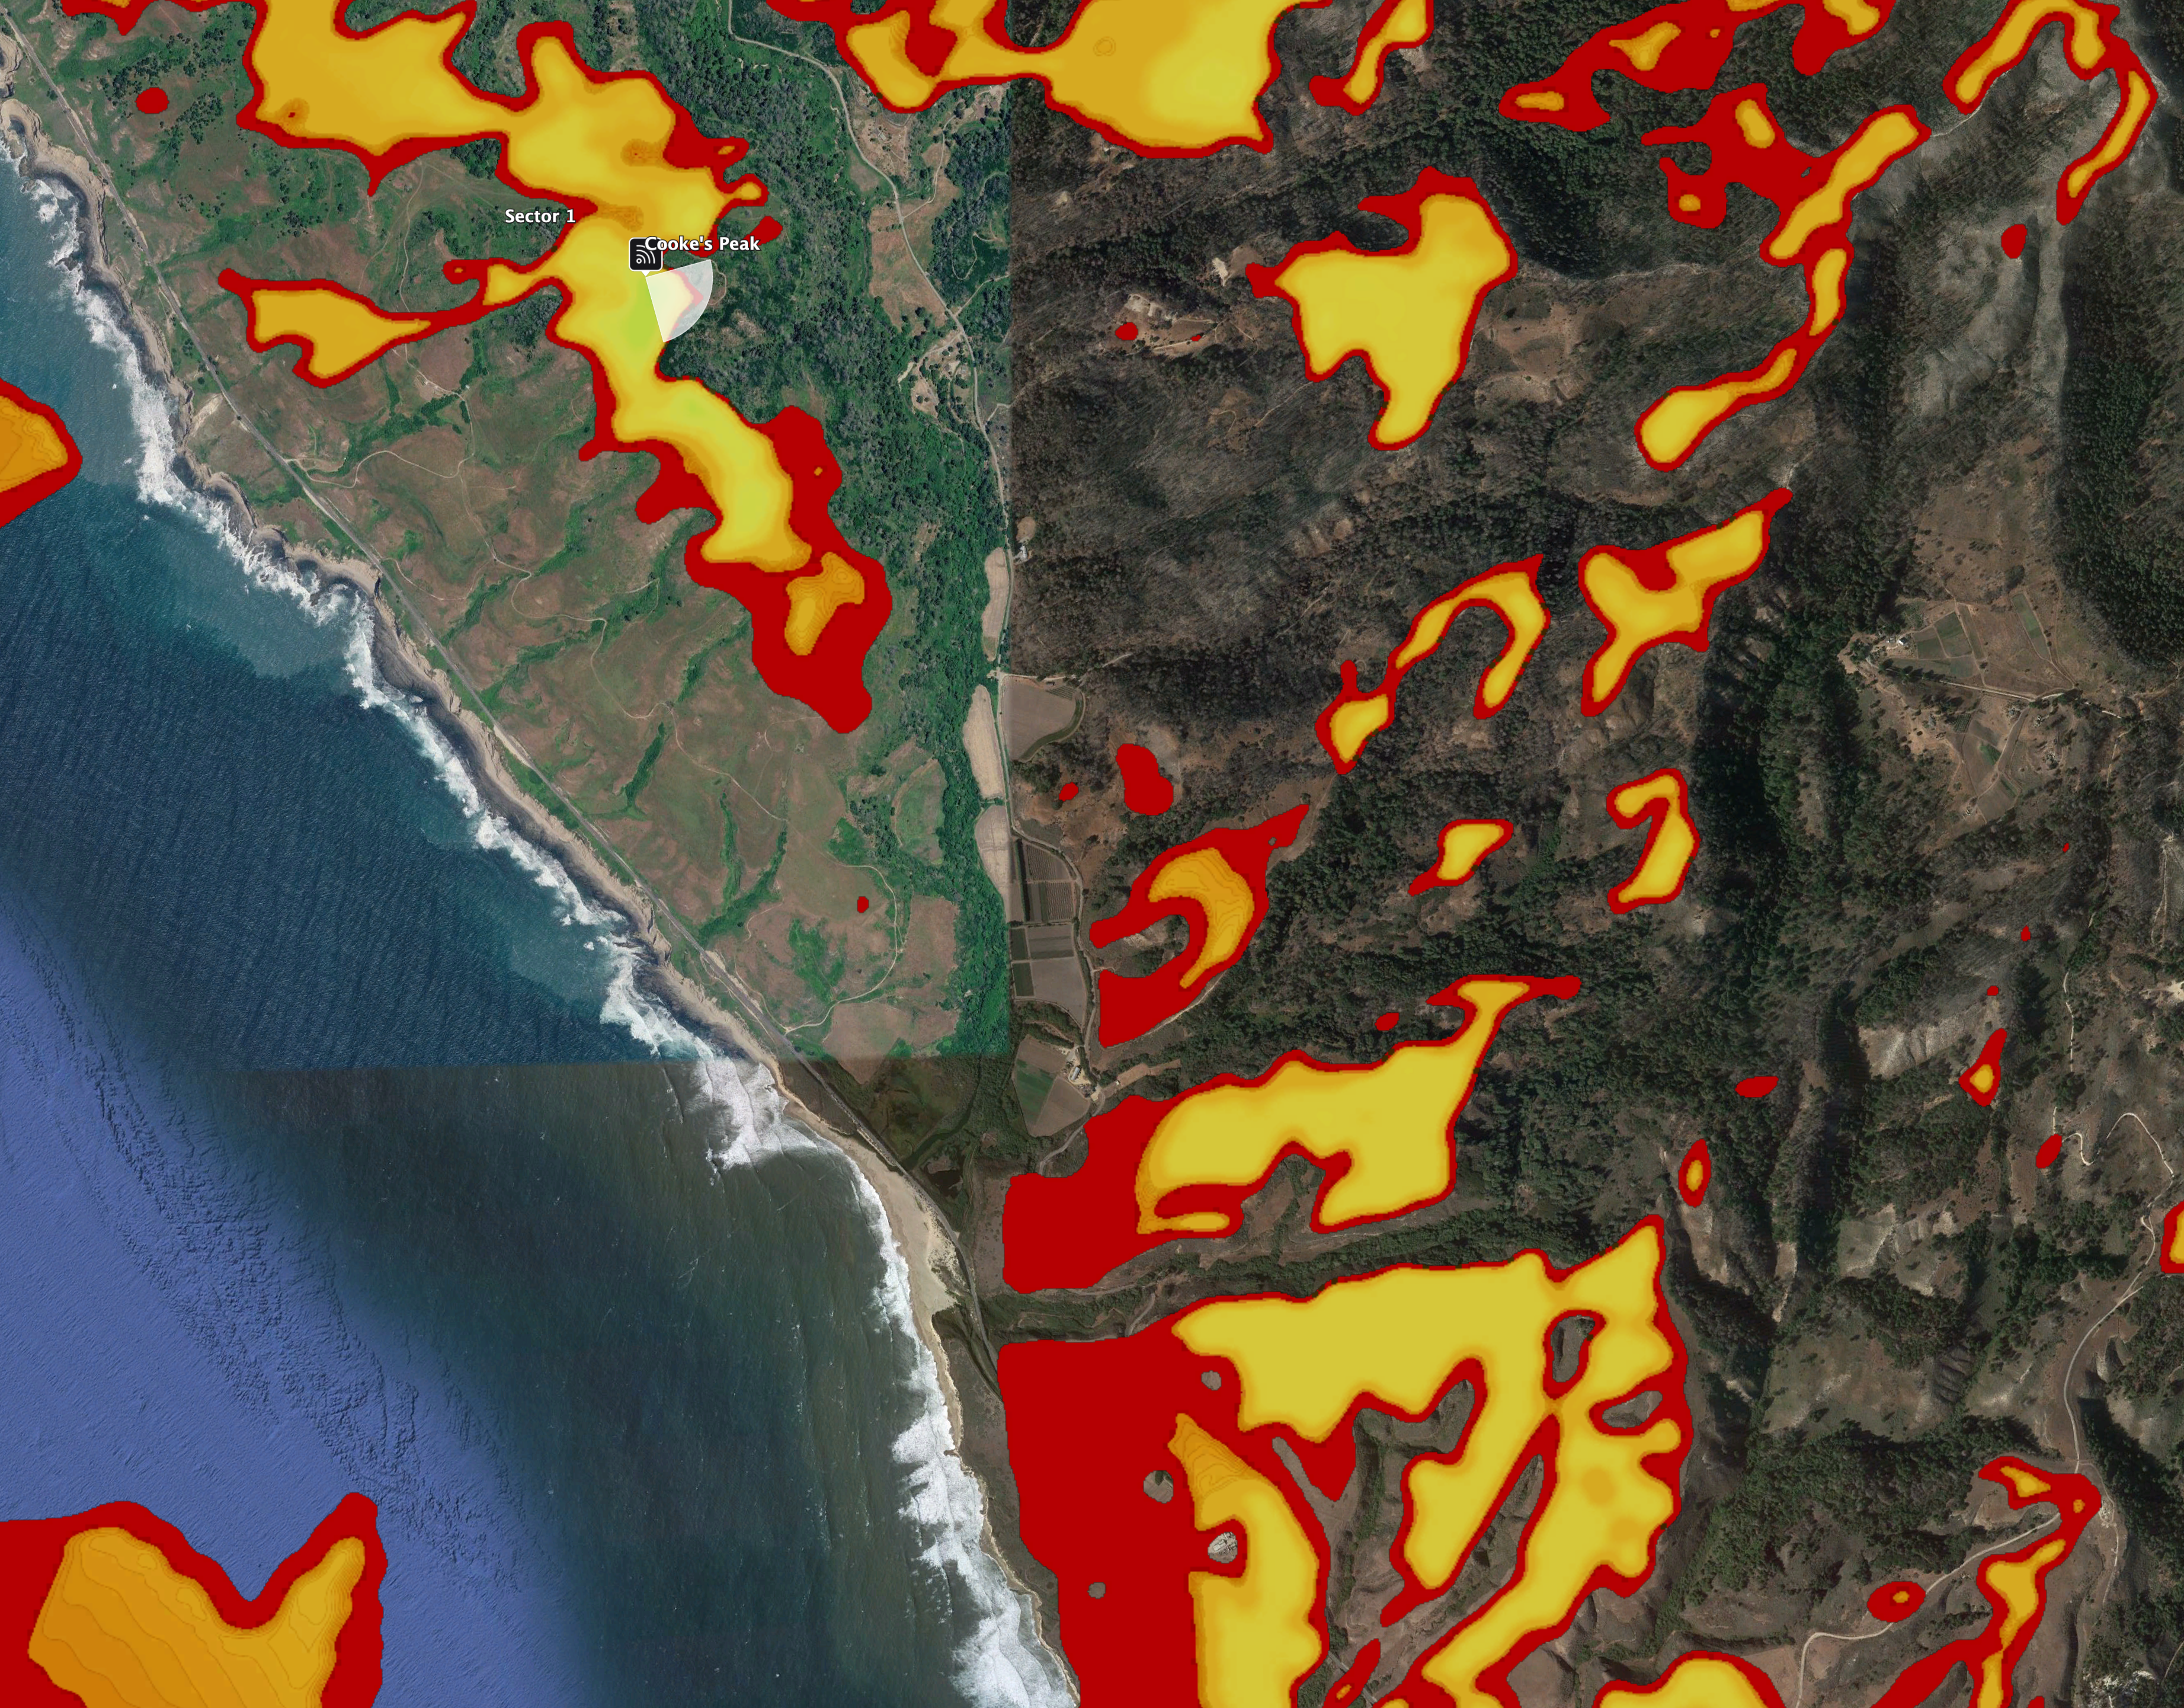
\includegraphics[max width=\linewidth]{Images/Eino Simulation Data.png}
    \caption[eino.ai RSRP simulation heatmap]{eino.ai RSRP simulation heatmap
    showing predicted coverage from Cooke's Peak with 120-degree SSE sector
    heading.}
    \label{fig:eino_heatmap}
\end{figure}

The simulation shows a pattern consistent with expectations for a high-gain
sector antenna aimed SSE from a 243~m elevation point. Strong and good signal
(green and yellow zones) is predicted in a roughly circular area immediately
surrounding Cooke's Peak, extending outward along the main coverage lobe in the
120-degree heading. Fringe signal (orange and red zones) reaches further south
along the coastal corridor and into portions of the valley. Terrain shadow zones
appear east and north of the deployment site where the terrain blocks direct line
of sight.

The simulation was used to confirm the antenna azimuth heading and to estimate
where additional radio placements would be needed to fill coverage gaps. It was
not used as a precise quantitative prediction, as the antenna model mismatch and
the difficulty of accurately modeling coastal vegetation attenuation introduce
known inaccuracies.

\subsection{SIM and Security Design}

PLMN selection for a CBRS private network follows a specific convention. The
OnGo Alliance, the CBRS industry group, has designated PLMN 315-010 as the
standard identifier for US private CBRS networks \autocite{hpe2019cbrsnetwork}.
This PLMN is analogous to the use of private IP address ranges like 10.0.0.0/8
in TCP/IP networks: it is not globally routable, it is available for any private
CBRS operator, and it is recognized by CBRS-capable devices as a local private
network. Using 315-010 ensures that UEs configured for this PLMN attempt to
register on the Swanton network when it is available, rather than scanning for
commercial carriers.

The team programmed three SIM cards, one per test device, with the following
IMSI assignments:

\begin{itemize}
    \item PHONE-10: IMSI 315010000000010
    \item PHONE-20: IMSI 315010000000020
    \item PHONE-30: IMSI 315010000000030
\end{itemize}

Each SIM stores the IMSI, Ki, and OPc values. All three SIMs used the same Ki
and OPc values for lab simplicity. In a production deployment, each SIM would
have a unique Ki.

Authentication uses the Milenage AKA protocol \autocite{hpe2019cbrssignaling}.
When a UE attempts to attach, the MME retrieves the subscriber record from the
HSS and generates an authentication challenge. The UE computes a response using
its SIM-stored Ki and OPc through the Milenage algorithm, and the MME
independently computes the expected response. If the values match, the UE is
authenticated. The protocol is mutual: the UE also verifies the network's
identity. Critically, neither the Ki nor the OPc is ever transmitted over the
air or over the S1 interface. A passive observer capturing all traffic cannot
recover the authentication keys or decrypt UE data traffic.

The APN ``internet'' was configured on the Android phones rather than programmed
onto the SIM cards. This is a practical choice for a lab and field-test
environment where the same SIMs might be used on different networks. On a
production ranch deployment, the APN could be pre-programmed on the SIM to
eliminate manual configuration.

% =============================================================================
\section{Test Plans}
% =============================================================================

\subsection{Phase 1: RF Propagation Simulation}

The first test phase used eino.ai to model signal coverage from Cooke's Peak
before any hardware was transported to the ranch.

\textbf{Tool:} eino.ai cloud-native RF simulation \autocite{einoai2024}.

\textbf{Method:} Place AP at Cooke's Peak with the antenna configuration
described in Section~IV.D, define a simulation area covering the ranch and
surrounding terrain, and compute the RSRP heatmap.

\textbf{Pass criterion:} RSRP $>-110$~dBm (marginal or better) at the main
ranch valley floor from a single radio at Cooke's Peak, confirming that the
site is viable.

\textbf{Output:} Georeferenced KMZ export (Eino Data Export.kmz) for overlay
with field data in Google Earth.

\subsection{Phase 2: Field Drive Test}

The second test phase collected measured RSRP data across the ranch during the
May~2 deployment.

\textbf{Tool:} G-NetTrack Lite \autocite{gnettrack} on three Android phones (UE~1,
UE~2, UE~3).

\textbf{Method:} All three phones were carried by the team during a walk/drive
test across the ranch. G-NetTrack logged RSRP, GPS coordinates, serving network
operator, and network technology at approximately ten-second intervals. Data was
collected across two separate route segments throughout the afternoon.

\textbf{Data processing:} A Python script (\texttt{clean\_drive\_test\_data.py})
filtered the raw logs to retain only rows where the serving operator was
``Swanton\_Ranch,'' where RSRP was between $-130$ and $-50$~dBm (valid LTE
range), and where the GPS coordinates fell within the ranch bounding box.
No-coverage points (rows where the operator was \texttt{NO\_COVERAGE}, T-Mobile,
AT\&T, or Verizon) were retained as gray reference markers. The script exported
both per-session KML files and a combined KML covering all UEs and sessions.

\textbf{Pass criterion:} Coverage pattern consistent with the eino.ai simulation
prediction; signal at the key working areas of the ranch.

\subsection{Phase 3: Throughput Testing}

\textbf{Tool:} OpenSpeedTest, a self-hosted Docker container running on the
Intel NUC at port 3000 \autocite{waveriders2025open5g2go}.

\textbf{Method:} Run a download and upload speed test from each connected phone
to the NUC directly over the LTE link. Running the test server locally on the
NUC isolates LTE performance from Starlink variability: the result reflects the
LTE link throughput, not the upstream internet speed.

\textbf{Pass criterion:} Download throughput $>10$~Mbps, consistent with the
engineering specification in Table~\ref{tab:engspec}.

\subsection{Failure Mode and Effects Analysis}

Table~\ref{tab:fmea} shows the FMEA for key system components.

\begin{table}[!ht]
    \centering
    \caption[Failure mode and effects analysis]{Failure mode and effects
    analysis (FMEA) for key system components.}
    \vspace{0.5\baselineskip}
    \begin{tabular}{p{0.14\linewidth}p{0.14\linewidth}p{0.14\linewidth}
                    p{0.08\linewidth}p{0.09\linewidth}p{0.20\linewidth}}
        \toprule
        \textbf{Component} & \textbf{Failure Mode} & \textbf{Effect}
            & \textbf{Severity} & \textbf{Prob.} & \textbf{Mitigation} \\
        \midrule
        eNodeB (radio) & Physical damage from wind/weather
            & Loss of network & High & Low
            & Secure mounting, weatherproof enclosure \\
        \addlinespace
        eNodeB (radio) & Power supply instability
            & Radio reset, service interruption & High & Medium
            & Regulated power supply; verified during this deployment \\
        \addlinespace
        eNodeB (radio) & Overheating
            & Thermal throttle or shutdown & Medium & Low
            & Temperature-rated hardware; adequate ventilation \\
        \addlinespace
        Antenna & Cable disconnection
            & Loss of transmit/receive & High & Medium
            & Secure weatherproof connectors \\
        \addlinespace
        Antenna & Physical damage
            & Reduced gain, distorted pattern & Medium & Low
            & Secure mounting; IP65+ hardware \\
        \addlinespace
        Open5GS (core) & Software crash or misconfiguration
            & Authentication failure & High & Low
            & Docker restart policy; configuration backup \\
        \addlinespace
        SIM cards & Wrong APN or IMSI mismatch
            & No data service & Medium & Medium
            & Pre-deployment verification checklist \\
        \addlinespace
        Starlink & Internet outage
            & UE data to internet fails & Medium & Medium
            & Core functions continue locally \\
        \addlinespace
        CBRS spectrum & Navy preemption (Tier~1)
            & Full network shutdown & High & Low--Med
            & Secondary LoRaWAN backup (future work) \\
        \addlinespace
        Power supply & Generator fuel exhaustion
            & All systems down & High & Low
            & Monitor fuel; solar/battery for permanent install \\
        \bottomrule
    \end{tabular}
    \label{tab:fmea}
\end{table}

% =============================================================================
\section{Development and Construction}
% =============================================================================

\subsection{Hardware Assembly and Physical Installation}

Figure~\ref{fig:cooks_peak} shows the completed deployment at Cooke's Peak on
May~2, 2026. The AW3376-E-F sector antenna is mounted at the top of a portable
telescoping tripod mast, with the Nova~846 eNodeB body secured to the same mast
behind the antenna. Four black RF cables connect the radio's ANT0 through ANT3
ports to four of the eight antenna ports. The GPS antenna for TDD timing
synchronization is also connected.

\begin{figure}[!ht]
    \centering
    \rotatebox{-90}{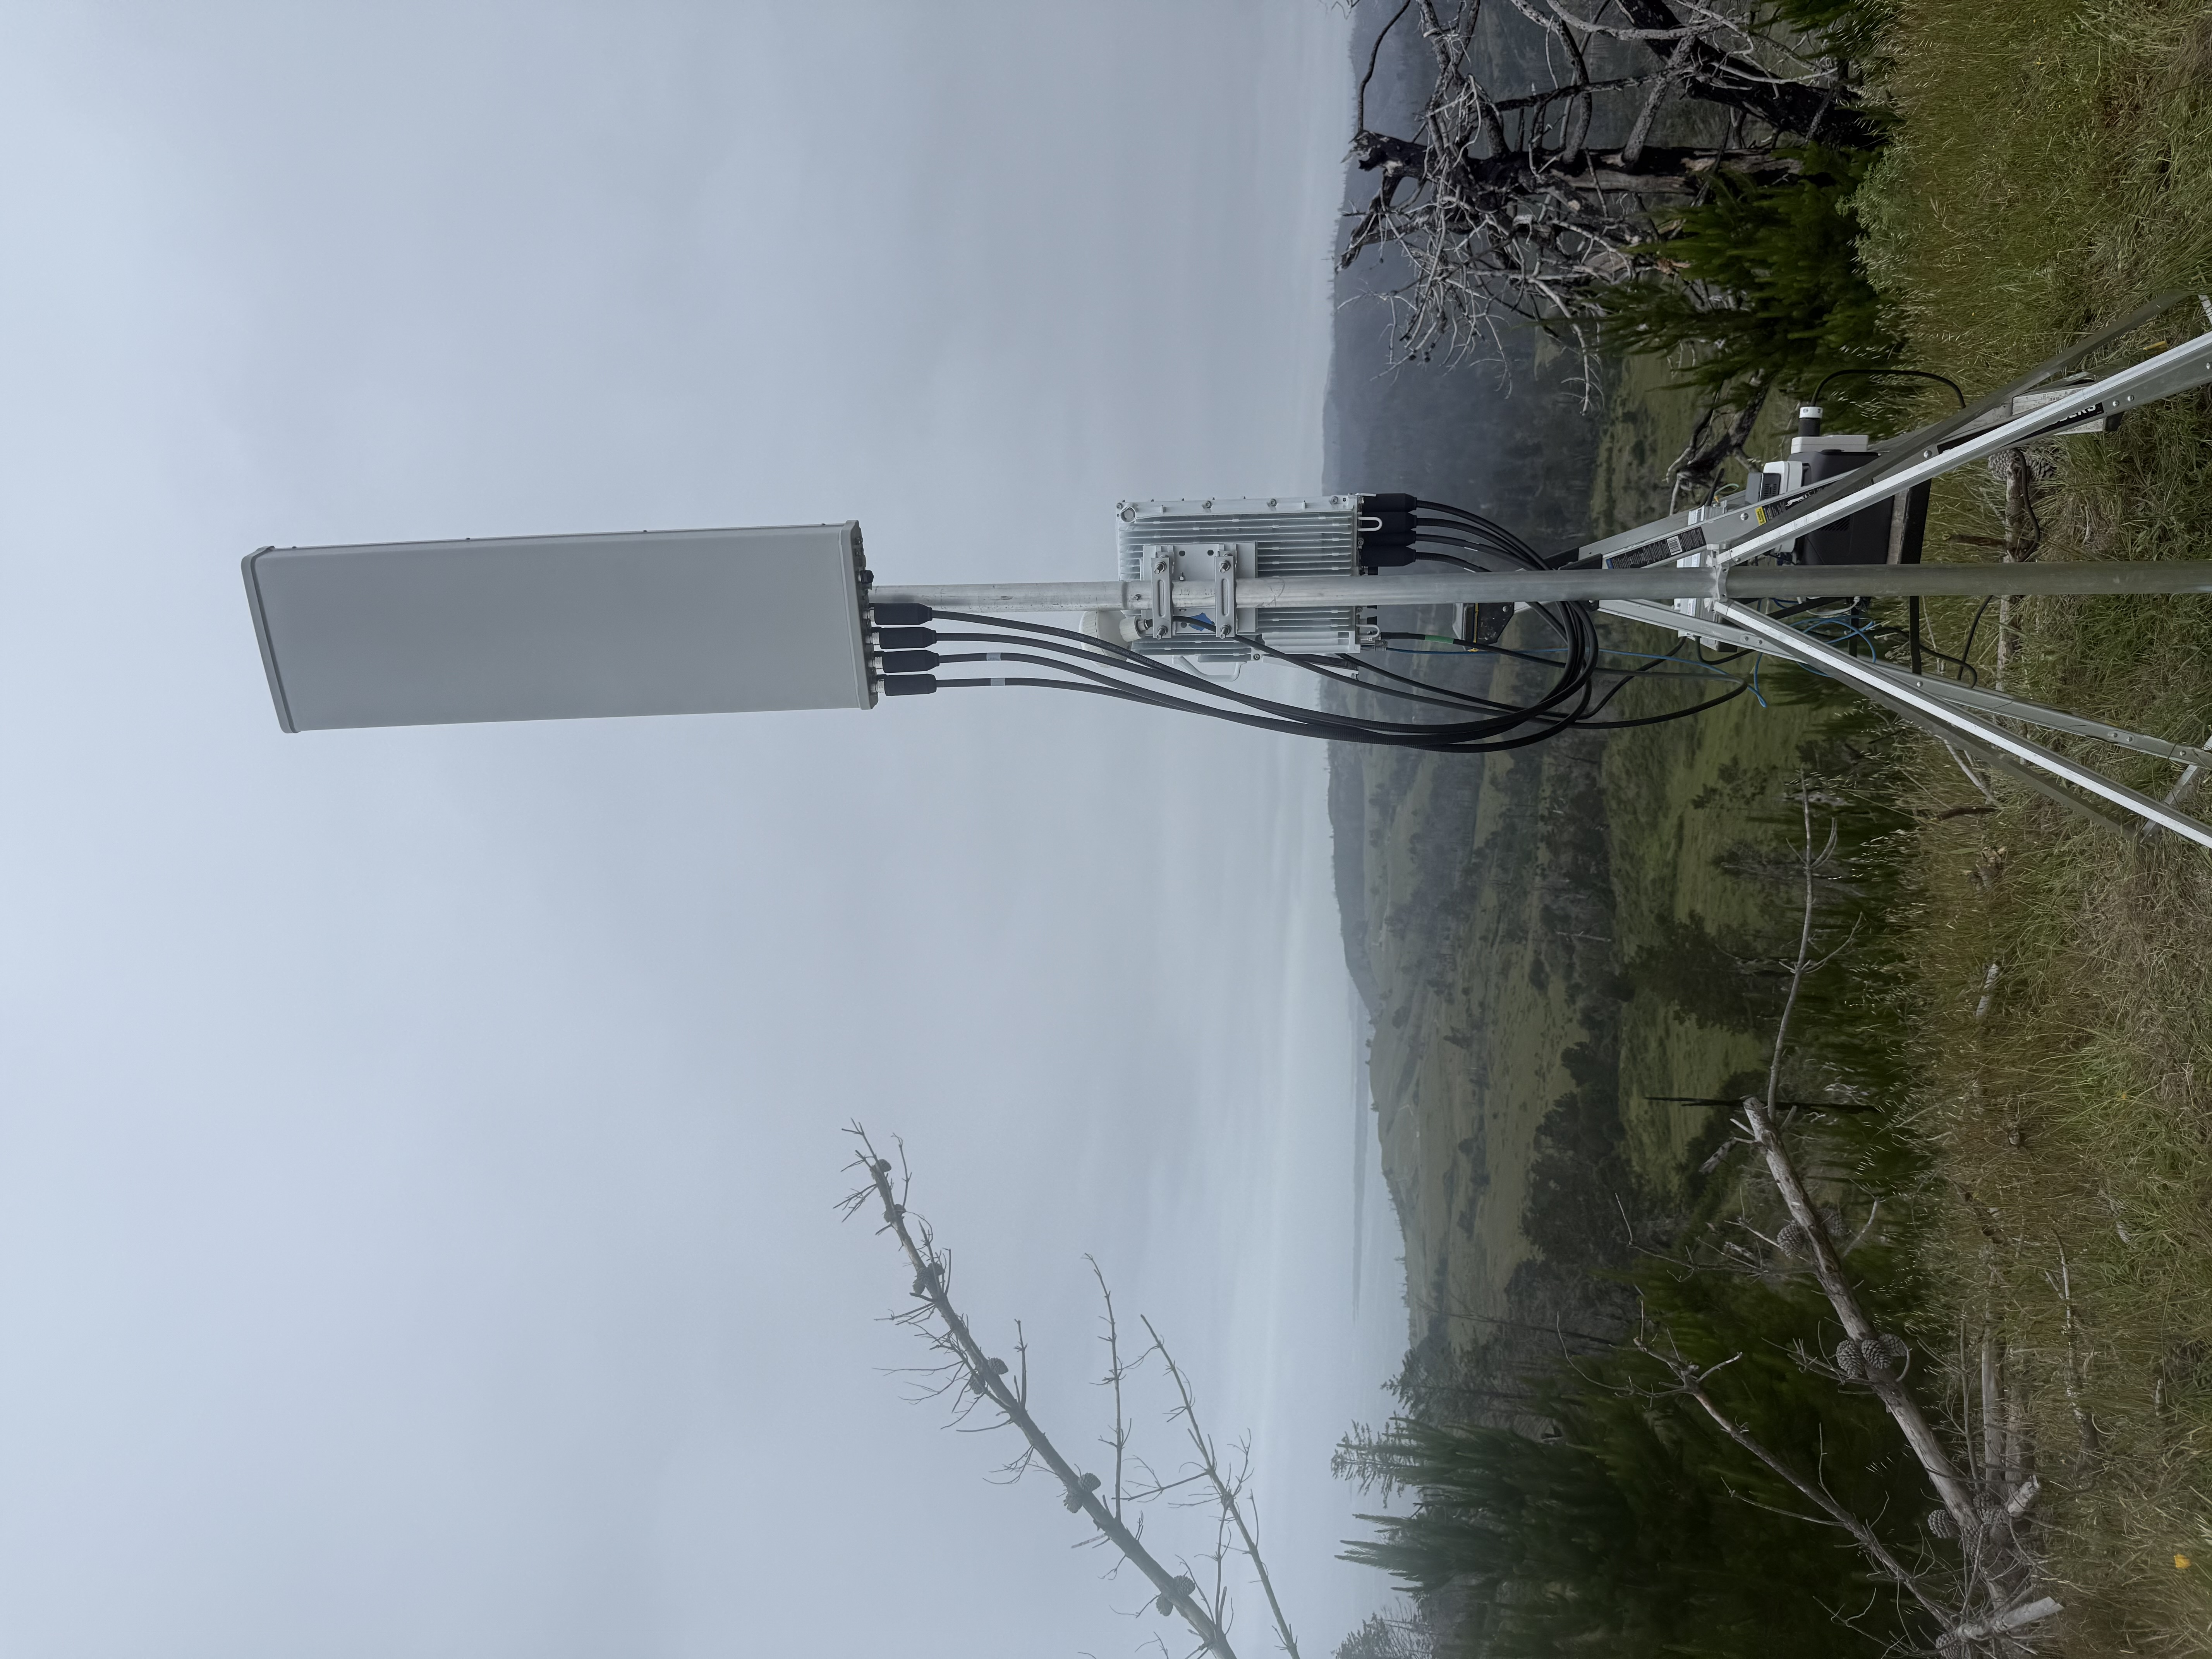
\includegraphics[height=\linewidth]{Images/IMG_3314.jpeg}}
    \caption[Nova 846 and AW3376-E-F antenna deployed at Cooke's Peak]{Baicells
    Nova 846 eNodeB with Alpha Wireless AW3376-E-F sector antenna mounted on
    portable tripod mast at Cooke's Peak, May~2, 2026.}
    \label{fig:cooks_peak}
\end{figure}

Figure~\ref{fig:lab_bench} shows the lab bench setup used during development,
with the Nova 430i, the Intel NUC running Open5GS, the private lab router,
and UE~1 visible.

\begin{figure}[!ht]
    \centering
    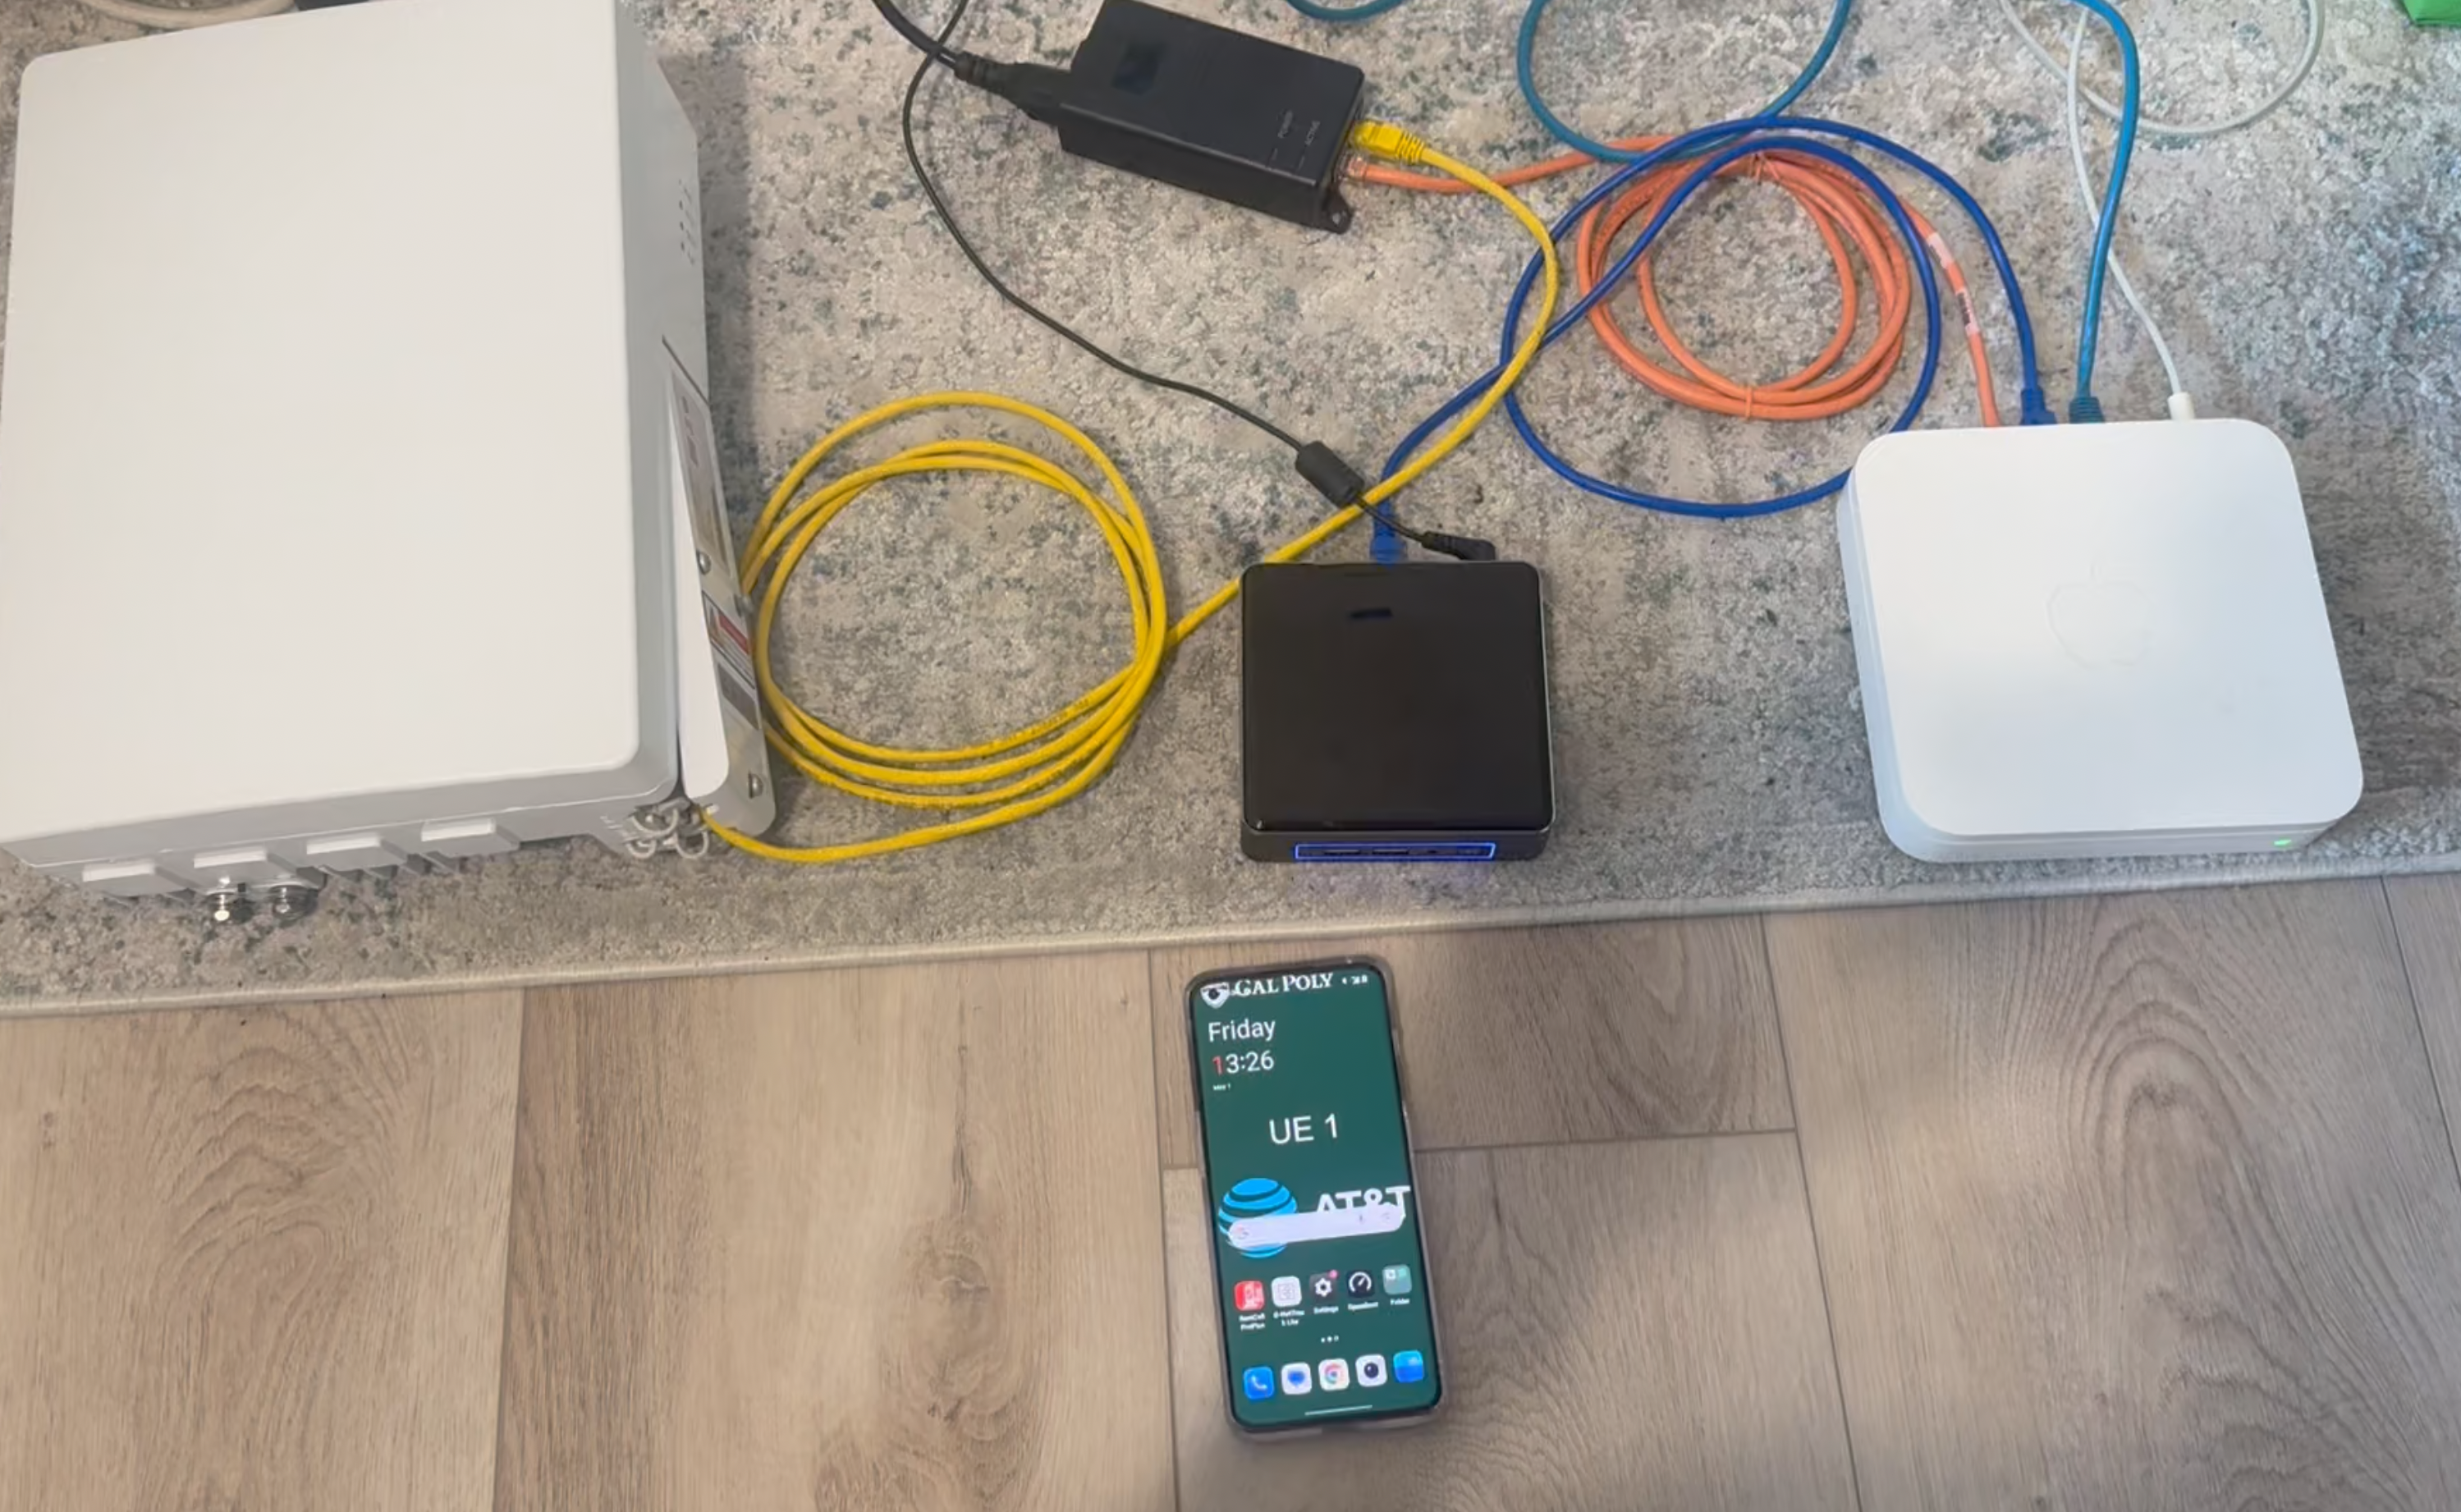
\includegraphics[max width=\linewidth]{Images/Nova 430i Test set up.png}
    \caption[Lab bench setup with Nova 430i, NUC, router, and UE 1]{Indoor lab
    bench setup during the development phase. Baicells Nova~430i (white box,
    left), Intel NUC running Open5GS (center), private LAN router (right),
    and UE~1 (front).}
    \label{fig:lab_bench}
\end{figure}

The tripod mast was set up at Cooke's Peak and secured. The AW3376-E-F antenna
was attached to the mast head, oriented with the face pointing 120~degrees
azimuth (SSE). The Nova 846 was secured to the mast below the antenna. RF cables
were connected from the radio's ANT0, ANT1, ANT2, and ANT3 ports to the antenna.
ANT4 through ANT7 were left unconnected, consistent with single-carrier mode
operation as documented in the Nova 846 installation guide
\autocite{baicells2023nova846}. The guide explicitly states that dual-carrier
mode requires ANT4 through ANT7, and that only ANT0 through ANT3 are active in
single-carrier mode. Leaving active transmit ports unconnected while the PA is
active would risk damaging the power amplifier, so this connection discipline is
important.

The GPS antenna was connected and oriented for sky view. The Intel NUC and
private router were co-located at the deployment site, connected via Ethernet.
The Starlink dish was positioned separately at a location with clear sky view
and connected to the router's WAN port.

Before enabling RF at any point during development or deployment, the team
followed a pre-RF safety checklist:

\begin{enumerate}
    \item ANT0 through ANT3 connected to antenna or dummy loads
    \item ANT4 through ANT7 disconnected (single-carrier mode only)
    \item Carrier mode set to Single Carrier
    \item HaloB disabled
    \item Cloud EPC disabled
    \item GPS synchronized
    \item MME connected and showing active status
    \item RF status set to OFF until all above confirmed
\end{enumerate}

During lab testing with dummy loads, this checklist prevented transmitting into
unloaded ports. During the Swanton deployment, it ensured GPS was synchronized
and that the core was confirmed running before any RF was enabled.

\subsection{Software Setup: Open5G2GO and Open5GS}

The core network software was installed and validated in the lab before transport
to the field.

\textbf{Operating system:} Ubuntu Server 22.04 LTS was installed on the Intel
NUC. After installation, SCTP kernel module support was verified:

\begin{verbatim}
sudo modprobe sctp
lsmod | grep sctp
\end{verbatim}

SCTP is required because the S1AP signaling between the eNodeB and the MME uses
SCTP on port~36412. Verifying SCTP availability before installing Open5GS
confirmed the kernel was ready.

\textbf{Docker:} Docker Engine was installed using the official convenience
script:

\begin{verbatim}
sudo apt install -y ca-certificates curl gnupg git
curl -fsSL https://get.docker.com | sudo sh
sudo usermod -aG docker $USER
\end{verbatim}

Open5G2GO and Open5GS run as a set of Docker containers. Using Docker means the
entire core network stack can be started, stopped, and updated as a unit, and
the configuration lives in a single \texttt{.env} file that is easily backed up.

\textbf{Open5G2GO installation:} The Waveriders installer handles the entire
Open5GS setup \autocite{waveriders2025open5g2go}:

\begin{verbatim}
curl -fsSL https://raw.githubusercontent.com/
  Waveriders-Collective/open5G2GO/main/install.sh | bash
\end{verbatim}

During the interactive install, the following configuration was specified:

\begin{itemize}
    \item Network mode: 4G LTE
    \item PLMN: 315-010
    \item UE IP pool: 10.48.99.0/24
    \item Ki and OPc: 32 hex ones (all-ones key, appropriate for lab use)
\end{itemize}

The installer produced a working Open5GS stack with a web management UI at
port~8080 and the MME listening on port~36412 SCTP.

\textbf{IP address migration:} During initial installation, the NUC was still on
the Wi-Fi network with IP address 192.168.12.86. After adding the dedicated lab
router and moving the NUC to the private LAN, the NUC received the final address
10.0.1.4. The Open5G2GO \texttt{.env} file still contained the old IP, so a
one-line search-and-replace updated both \texttt{DOCKER\_HOST\_IP} and
\texttt{HOST\_IP} variables. The stack was restarted to pick up the change:

\begin{verbatim}
cp .env .env.backup.$(date +%F-%H%M)
sed -i 's/192\.168\.12\.86/10.0.1.4/g' .env
docker compose -f docker-compose.prod.yml down
docker compose -f docker-compose.prod.yml up -d
\end{verbatim}

The final configuration visible in the web UI at \texttt{http://10.0.1.4:8080}
showed: PLMN ID 315010, MME IP 10.0.1.4 on port~36412, APN ``internet,'' UE IP
pool 10.48.99.0/24.

\textbf{OpenSpeedTest:} A self-hosted speed test server was deployed on the NUC
for local throughput testing:

\begin{verbatim}
docker run --restart=unless-stopped --name openspeedtest \
  -d -p 3000:3000 openspeedtest/latest
\end{verbatim}

The \texttt{-{}-restart=unless-stopped} flag ensures the container starts
automatically after a reboot. The test server was accessible at
\texttt{http://10.0.1.4:3000} from any connected UE.

\subsection{Subscriber Configuration and SIM Provisioning}

Three subscribers were added to Open5GS through the Open5G2GO web UI. Each
subscriber entry specifies a name, IMSI, static UE IP address, and APN. The
static IP assignments use a scheme where the last two digits of the IMSI match
the last octet of the IP address, making troubleshooting straightforward.

\begin{table}[!ht]
    \centering
    \caption[Subscriber configuration]{Subscriber configuration.}
    \vspace{0.5\baselineskip}
    \begin{tabular}{lccc}
        \toprule
        \textbf{Name} & \textbf{IMSI} & \textbf{UE IP} & \textbf{APN} \\
        \midrule
        PHONE-10 & 315010000000010 & 10.48.99.10 & internet \\
        PHONE-20 & 315010000000020 & 10.48.99.20 & internet \\
        PHONE-30 & 315010000000030 & 10.48.99.30 & internet \\
        \bottomrule
    \end{tabular}
    \label{tab:subscribers}
\end{table}

A Gialer USB SIM writer running GRSIMWrite was used to program three blank
programmable SIM cards. The SIM programming procedure used the LTE/WCDMA
parameter panel in GRSIMWrite rather than the GSM panel:

\begin{enumerate}
    \item Insert blank SIM and click Read Card to confirm successful read
    \item In the LTE/WCDMA panel: set IMSI15 format (not IMSI18), enter IMSI,
    Ki, and OPc values; select OPc mode (not OP); confirm Milenage algorithm
    \item Click Write Card
    \item Click Read Card again to verify the written values against what was
    entered
    \item Label the physical SIM with the PHONE number
\end{enumerate}

The APN ``internet'' was configured manually in each Android phone's mobile
network settings (Name: Open5G2GO; APN: internet).

\subsection{Baicells Nova 430i Configuration (Lab Validation)}

The Nova~430i was used as the first radio in the development process. Working
with the 430i first served an important risk-management purpose: it allowed the
team to verify that the Open5GS core, SIM cards, and Android phone configuration
all worked together before introducing the higher-power, more complex Nova 846.

The key configuration changes from the 430i's factory defaults were:

\begin{itemize}
    \item Country Code: changed from ``USA-FCC(CBRS) - Domain Proxy'' to
    ``Other'' (disables SAS requirement for lab use)
    \item HaloB: OFF (the factory default is ON; HaloB must be disabled to use
    an external core)
    \item Cloud EPC: OFF
    \item PLMN: changed from 314030 to 315010
    \item MME IP: changed from 127.0.0.1 to 10.0.1.4
    \item MME PLMN: 315010; S1 Link Port: 36412; TAC: 1
    \item Band: 48; Bandwidth: 20~MHz; EARFCN: 55990 (3625~MHz)
\end{itemize}

After applying these changes, the 430i showed MME Status: Connected, confirming
S1AP communication with Open5GS was working. With all three phones confirmed
attached and accessing the internet through the 430i, the lab validation phase
was complete.

\subsection{Baicells Nova 846 Configuration (Swanton Deployment)}

The Nova 846 was configured to match the 430i's working configuration as closely
as possible, with changes specific to the outdoor deployment environment. The
relevant changes from factory defaults were:

\begin{itemize}
    \item HaloB: OFF; Cloud EPC: OFF; Country Code / SAS: Other
    \item PLMN: 315010; MME IP: 10.0.1.4; MME PLMN: 315010; TAC: 1
    \item Band: 48; Bandwidth: 20~MHz; EARFCN: 56290 (3655~MHz)
    \item TDD SubFrame Assignment: 2 (3:1 DL:UL ratio)
    \item Special SubFrame Pattern: 7
    \item Carrier mode: Single Carrier; Active ports: ANT0--ANT3
    \item eNB ID: 288392; PCI: 121; Cell ID: 193
    \item LGW: ON, NAT mode
\end{itemize}

\textbf{GPS synchronization:} TDD operation requires precise time
synchronization. The Nova 846 derives this timing from GPS. Before enabling RF,
the GPS antenna was connected with clear sky view, and the web UI was monitored
until it showed GPS Sync Status: Synchronized. RF was not enabled until GPS sync
was confirmed.

After applying all configuration changes, the MME status showed Connected, GPS
showed Synchronized, and the pre-RF checklist was complete. RF was enabled and
PHONE-10 attached to the \textit{Swanton\_Ranch} network, confirmed by the
Open5G2GO web UI showing Registered UEs: 1 and PHONE-10 connected with IP
10.48.99.10.

\subsection{Power System}

The radio's power draw during active operation peaked at approximately 70~W,
measured on a power meter in between the battery and radio. This figure accounts
for the radio PA and baseband processing but does not include the NUC, router,
or Starlink terminal. The breakdown by component:

\begin{itemize}
    \item Nova~846 (4T4R): $4 \times 10$~W per channel = 40~W RF output power,
    plus baseband processing overhead. Total 60 to 70~W
    \item Intel NUC: approximately 15 to 25~W under moderate load
    \item Private router: approximately 5 to 10~W
    \item Starlink terminal: approximately 50 to 75~W (varies with dish
    generation)
    \item Total system: Peaks at 105~W, averages to 92.5~W (not including
    Starlink terminal since it won't be the main internet backhaul)
\end{itemize}

\textbf{Deployment day power source:} On May~2, the radio and Starlink terminal
were powered by the battery system on a travel trailer, while the NUC and router
were powered by a smaller portable battery bank.

For a permanent installation, the power system design would center on a solar
array, battery bank, and Maximum Power Point Tracking (MPPT) charge controller sized for the full system load
plus margin for coastal overcast days. A 200~W solar panel array with a 100~Ah
lithium battery bank would provide continuous operation through several
consecutive cloudy days at the estimated system load.

The power efficiency of the Nova~846 relative to legacy macro cellular
infrastructure is worth noting. A traditional macro base station delivering
comparable coverage would require several hundred watts of transmit power. The
Nova~846 achieves kilometer-scale coverage at 40~W of radiated power,
making solar-powered operation at a remote site feasible.

% =============================================================================
\section{Integration and Test Results}
% =============================================================================

\subsection{Deployment Day: May 2, 2026}

The deployment team arrived at Cooke's Peak at Swanton Pacific Ranch in the
early afternoon of May~2, 2026. Setup of the antenna mast, radio, NUC, and
Starlink required approximately one hour from arrival to network-up.

The bring-up sequence followed the pre-RF checklist described in
Section~VI.A. The NUC was powered first and Open5G2GO was confirmed running.
The Nova~846 was powered via its dedicated 48~V DC power supply input and
allowed several minutes to acquire GPS sync. Once the web UI showed GPS Sync
Status: Synchronized and MME Status: Connected, RF was enabled.

\textbf{Power supply issue:} Shortly after initial RF enable, the radio began
cycling on and off. The web UI showed intermittent MME disconnects corresponding
to the radio resets. Investigation found that the power supply connection to the
radio was unstable. After correcting the power connection and securing it firmly,
the radio stabilized and maintained continuous operation for the remainder of
the deployment. This issue directly informs the power system design for the
permanent installation, as discussed in Section~VII.E.

Drive testing was conducted throughout the afternoon with all three phones
active. UE~2 was carried during the test but, as discussed in Section~VII.E,
produced no data due to a logging failure that was not detected until
post-deployment data review.

\subsection{Coverage Measurement Results}

The raw G-NetTrack logs from all sessions were processed by
\texttt{clean\_drive\_test\_data.py}. The script retained only
\textit{Swanton\_Ranch}-operator rows within the valid RSRP range and the
geographic bounding box, and collected no-coverage reference points. The
combined output, \texttt{ALL\_combined\_rxlev.kml}, contains the data visualized
in Figure~\ref{fig:drive_test}.

Figure~\ref{fig:drive_test} shows the cleaned drive test RSRP data plotted on
the USGS topographic base map \autocite{usgs2026topo}. Colored dots represent
\textit{Swanton\_Ranch} signal, graded by strength. Gray dots represent
locations where data was collected but the phone was either on a commercial
network or showing no coverage. The route extends approximately 4~km
north-south and 1.9~km east-west.

\begin{figure}[!ht]
    \centering
    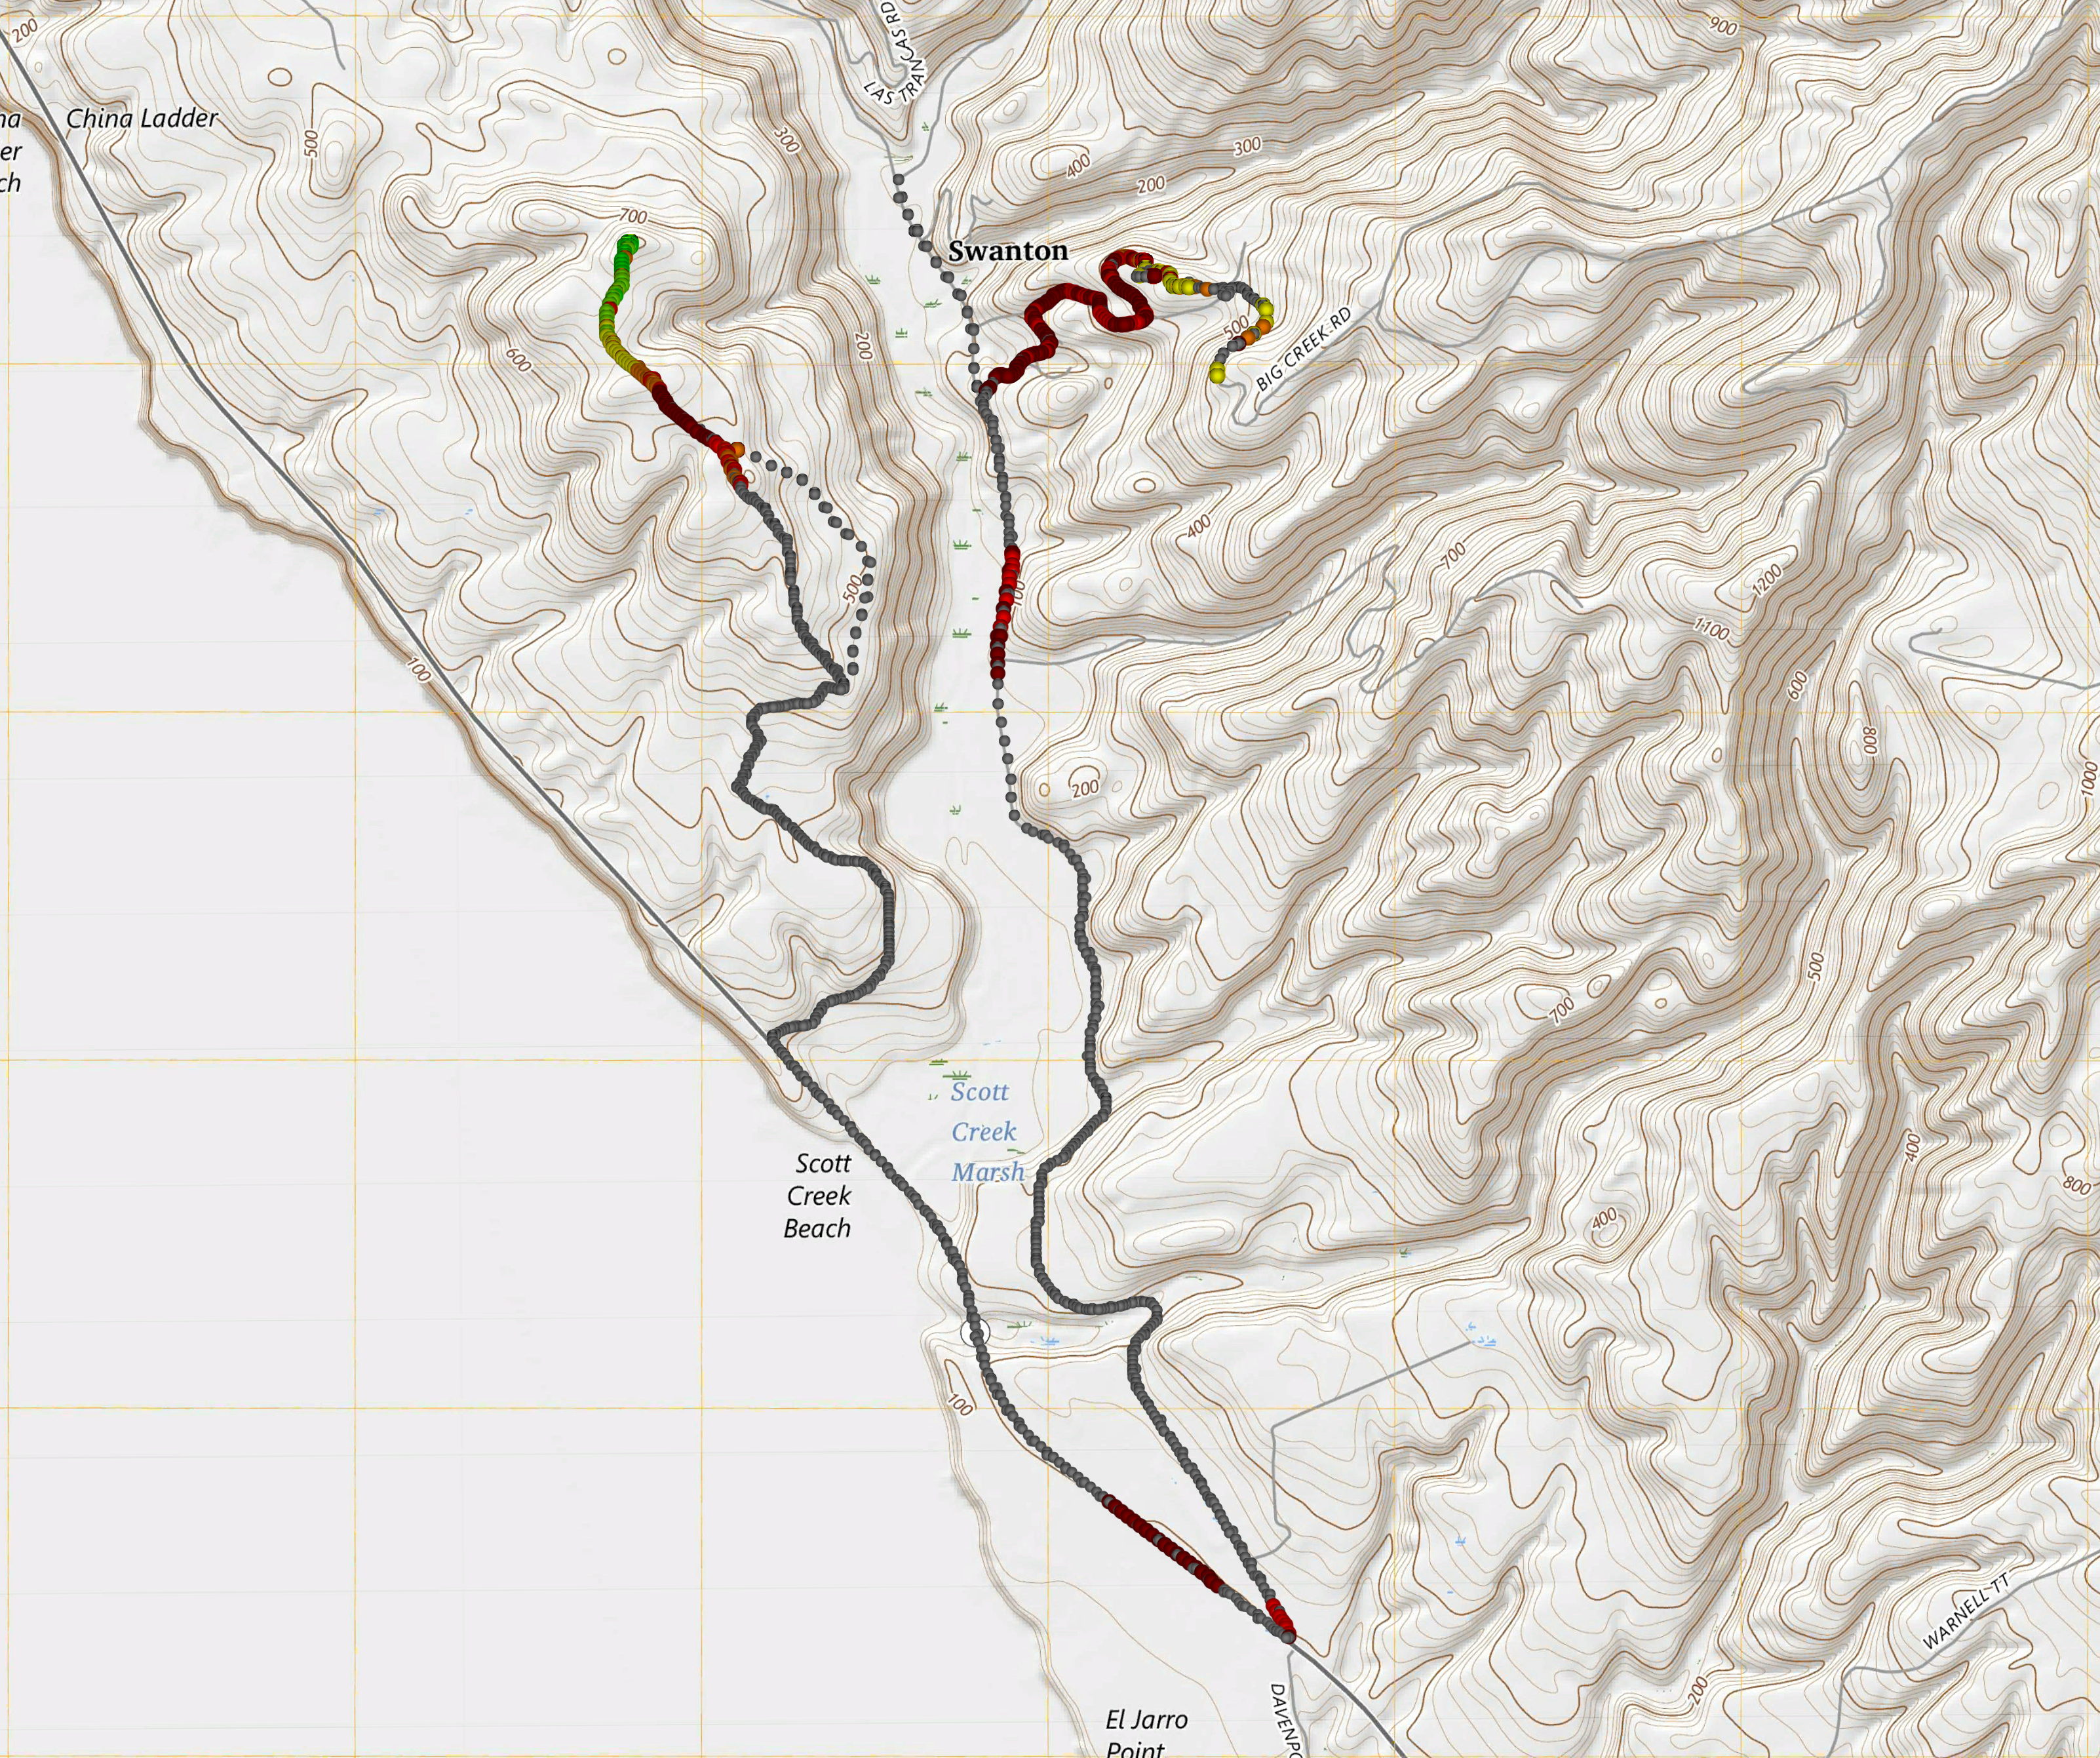
\includegraphics[max width=\linewidth]{Images/UE Walk Test Data.png}
    \caption[Measured drive test RSRP on USGS topographic base]{Measured drive
    test RSRP data overlaid on USGS topographic base map. Colored dots:
    \textit{Swanton\_Ranch} signal. Gray dots: no-coverage reference
    points.}
    \label{fig:drive_test}
\end{figure}

Table~\ref{tab:rsrp_dist} shows the RSRP distribution across all 1,655 valid
signal measurements.

\begin{table}[!ht]
    \centering
    \caption[Measured RSRP distribution]{Measured RSRP distribution across all
    1,655 valid Swanton\_Ranch signal measurements.}
    \vspace{0.5\baselineskip}
    \begin{tabular}{lccc}
        \toprule
        \textbf{RSRP Range} & \textbf{Quality} & \textbf{Count}
            & \textbf{Percentage} \\
        \midrule
        $>-80$~dBm           & Strong    & 308   & 18.6\% \\
        $-80$ to $-90$~dBm   & Good      & 106   & 6.4\%  \\
        $-90$ to $-100$~dBm  & Fair      & 228   & 13.8\% \\
        $-100$ to $-110$~dBm & Marginal  & 449   & 27.1\% \\
        $-110$ to $-120$~dBm & Weak      & 278   & 16.8\% \\
        $-120$ to $-130$~dBm & Very Weak & 286   & 17.3\% \\
        \midrule
        \textbf{Total (Swanton\_Ranch signal)} & & \textbf{1,655} & \textbf{100\%} \\
        No coverage (within bounding box)      & & 4,080          & ---            \\
        \bottomrule
    \end{tabular}
    \label{tab:rsrp_dist}
\end{table}

The combined signal and no-coverage dataset contains 5,735 georeferenced
measurement points. Coverage was present at approximately 29~percent of measured
locations. Strong and good signal was concentrated near Cooke's Peak, degrading
to marginal and weak as the route moved south and southeast.

UE~2 produced no data. The log files were zero bytes when retrieved
post-deployment. The cause is unknown; this is addressed as a lesson learned in
Section~VII.E.

\subsection{Simulation vs.\ Measured Comparison}

Figure~\ref{fig:overlay} overlays the drive test RSRP measurements directly on
the eino.ai simulation heatmap, using a hybrid topo/satellite base map in Google
Earth.

\begin{figure}[!ht]
    \centering
    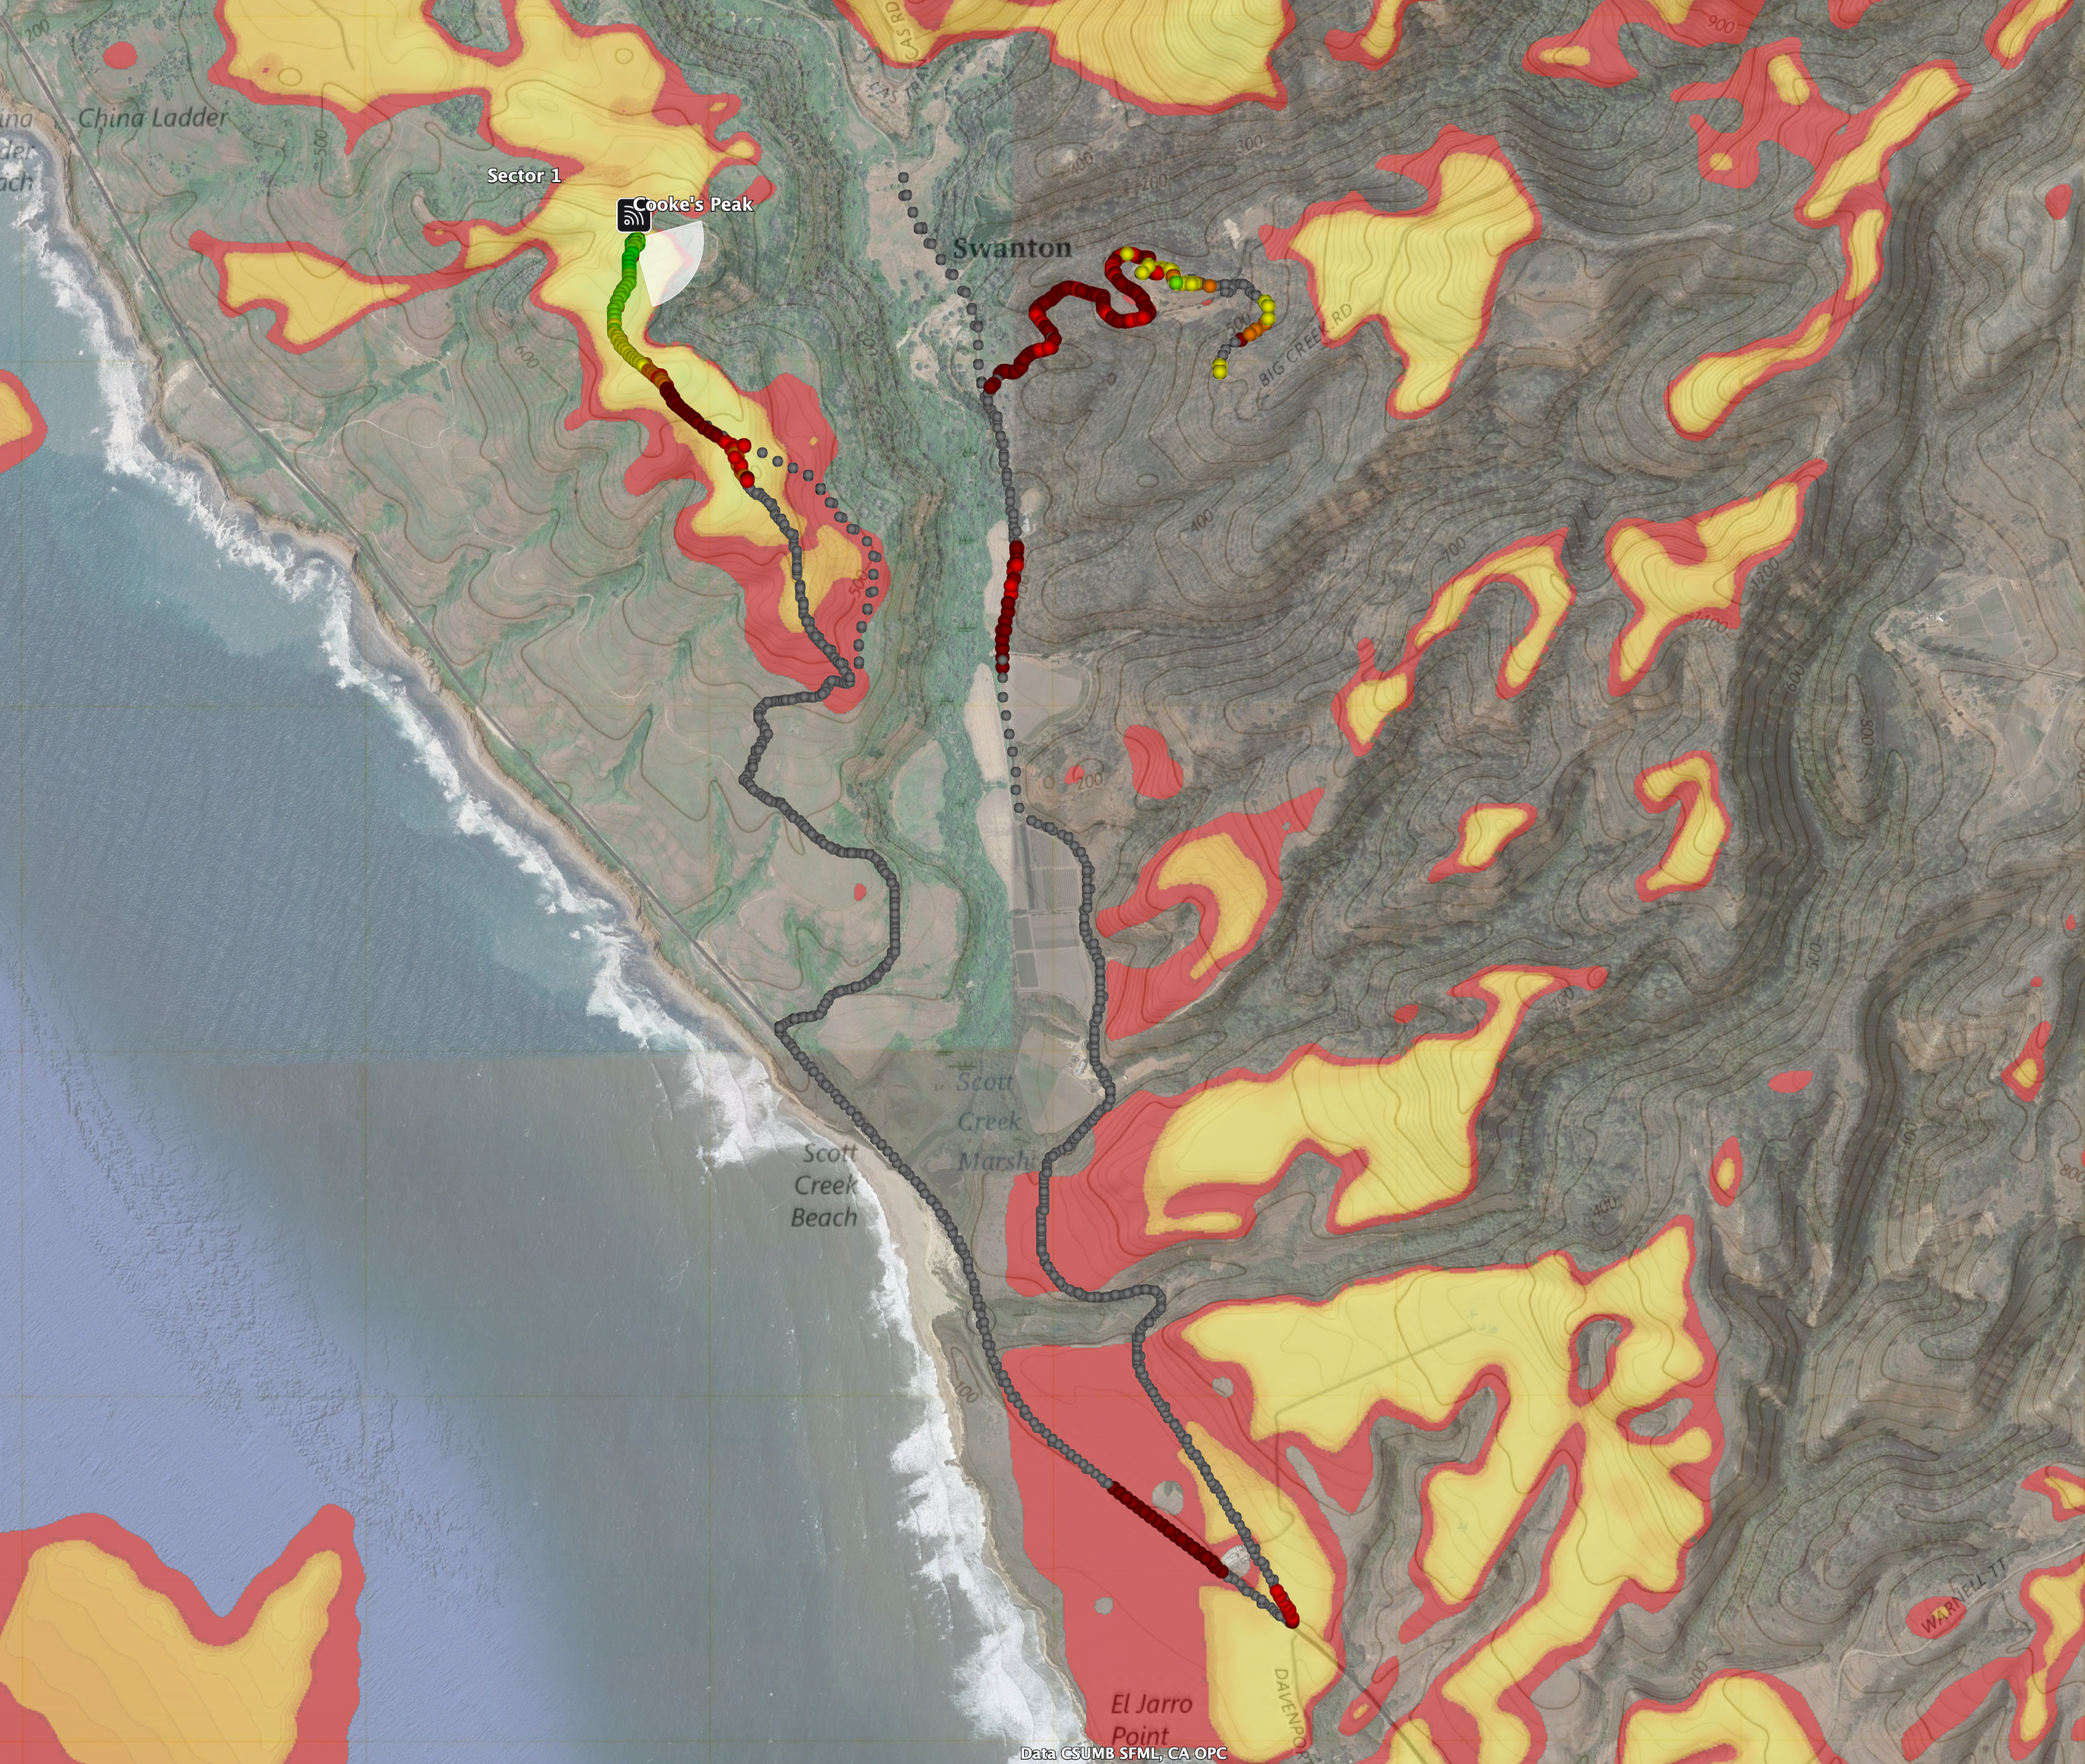
\includegraphics[max width=\linewidth]{Images/Eino and UE data overlaid.png}
    \caption[Simulation and measured coverage overlaid]{Drive test RSRP
    measurements overlaid on eino.ai simulation heatmap showing agreement
    near Cooke's Peak and simulation overestimation of coverage range.}
    \label{fig:overlay}
\end{figure}

\textbf{Where simulation and measurement agree:}

Near Cooke's Peak, the colored drive test dots fall within the corresponding
colored zones of the eino.ai heatmap. Green and yellow drive test dots (strong
and good signal, $>-80$~dBm) appear within the eino.ai green and yellow zones.
The simulation also correctly predicted terrain shadow zones. Large areas east
of the coastal ridge show no predicted signal in the eino heatmap and no
\textit{Swanton\_Ranch} signal in the drive test.

\textbf{Where simulation and measurement diverge:}

Moving south from Cooke's Peak along the coastal corridor, the simulation
predicts fringe signal coverage (orange and red zones, $-100$ to $-120$~dBm)
across large areas. The drive test data shows predominantly no
\textit{Swanton\_Ranch} coverage in these same areas. The simulation's effective
coverage radius is substantially larger than what was measured.

\textbf{Likely causes of simulation overestimation:}

Two factors contribute to the discrepancy. First, the antenna gain mismatch: the
simulation used the KP Performance KPPA-3GHZ0P905-45 at 16.5~dBi, while the
deployed antenna has a rated gain of 15.5~dBi. A 1~dB reduction in antenna gain
corresponds to a 1~dB reduction in received signal strength at all ranges,
shifting the effective coverage radius inward. Second, environmental attenuation:
the eino.ai terrain model accounts for surface elevation but has limited
capability to model vegetation attenuation. The Swanton Ranch coastal terrain
combines recovering scrub, standing dead conifer from the 2020 fire, live
coastal Douglas-fir, and maritime fog conditions. The deployment day on May~2
was overcast, and some degree of atmospheric attenuation was likely present.

\textbf{Key conclusion:}

The simulation was a valuable planning tool. It correctly identified Cooke's
Peak as the best deployment site, correctly predicted the coverage direction and
near-field performance, and correctly identified the terrain shadow zones. It
overestimated coverage range, as expected for any RF simulation in complex
coastal terrain without site-specific calibration data. The practical implication
is that a single radio at Cooke's Peak covers roughly 29~percent of the measured
routes across the ranch. Full coverage will require at least one additional radio
placed to illuminate the areas that Cooke's Peak cannot reach due to terrain and
distance.

\subsection{Throughput Results}

Throughput tests were conducted at a few key locations during the deployment
using OpenSpeedTest on each UE phone, measuring upload and download rates as
well as response time. A total of three speed tests were taken, with the best
performance being 72.9~Mbps upload and 10.1~Mbps download. One result showed
just 37.9~Mbps up and 1.8~Mbps down. Each test showed approximately 35~ms
ping. The better two of these results satisfy the desired requirements and
expectations for the network; the low-end result was taken at a location with
worse reception.

\subsection{Lessons Learned}

Five lessons from the development and deployment process are worth documenting
specifically, because each one is a potential failure mode for the next team.

\textbf{1. Regulated power is essential for field eNodeB operation.}

The power supply instability that caused radio resets during the initial bring-up
was the most disruptive issue of the deployment. The Nova~846 reacts to power
supply noise and voltage fluctuations with radio resets and MME disconnects.
Because the initial deployment used a simple power supply with no further
regulation or noise reduction, this issue presented itself on multiple occasions
during the field test. For a permanent installation, the power system must
provide clean, stable DC within the radio's specified input voltage range. A solar-plus-battery system with a
proper MPPT charge controller and a DC-DC regulator on the radio power input is
the correct approach.

\textbf{2. LGW mode was required because the Open5GS SGW user-plane path did
not initialize correctly.}

The standard LTE user-plane path through Open5GS relies on the SGW creating a
GTP-U tunnel interface (\texttt{ogstun}) that appears as a virtual network
interface on the Linux host. In this project's configuration, that interface did
not appear, and user traffic from attached phones had no route to the internet.
Switching to Baicells LGW NAT mode resolved the data path problem. The root
cause was not fully diagnosed. For a production deployment, understanding and
resolving this issue is worthwhile because LGW mode bypasses Open5GS's traffic
management and visibility functions.

\textbf{3. GPS lock takes time; plan for it.}

The Nova~846 requires GPS synchronization before TDD RF operation can proceed
reliably. GPS acquisition from a cold start can take several minutes. If the
deployment schedule is tight, powering the radio before beginning antenna and
cable installation allows GPS acquisition to proceed in the background. This
issue also compounded the power supply issue, since it took several minutes for
the radio to reboot and acquire GPS lock every time it reset due to the
unreliable power supply.

\textbf{4. Verify G-NetTrack is actively logging before starting a drive test
route.}

UE~2 produced zero bytes of log data. The phone appeared to be running
G-NetTrack during the test but was not writing to the log file. This was not
detected until the post-deployment data review. Before starting any drive test
route, confirm that the log file is being written by checking file size growth
in the G-NetTrack log directory.

\textbf{5. Single-carrier 4T4R used; 8T8R dual-carrier is available as a future
upgrade.}

The Nova~846 supports two independent carriers with full 8T8R operation when
both ANT0--3 and ANT4--7 are connected to the antenna. Moving to dual-carrier
would double the available spectrum (two 20~MHz carriers) and potentially double
throughput capacity. The AW3376-E-F has all eight ports available, so this
upgrade path requires no new hardware.

% =============================================================================
\section{Conclusion}
% =============================================================================

\subsection{What Was Achieved}

This project produced the first working private LTE network at Swanton Pacific
Ranch. The complete technology stack was demonstrated: a Baicells Nova~846
outdoor macro eNodeB, an Open5GS core network running on a local Intel NUC, SIM
cards programmed with PLMN 315-010 credentials, and three Android devices
successfully attached and routing data over the LTE link. Internet connectivity
through Starlink was confirmed.

The team collected 1,655 valid RSRP measurements from the
\textit{Swanton\_Ranch} network across 4~km of ranch terrain using G-NetTrack
Lite on two test devices. An eino.ai RF propagation simulation was completed
prior to deployment and compared against the field data, producing a quantitative
assessment of simulation accuracy at this site. The simulation correctly
characterized near-field performance and terrain shadow zones, and overestimated
coverage range by a margin consistent with the identified antenna gain mismatch
and environmental factors.

All configuration details---including Open5GS parameters, eNodeB settings, SIM
programming procedures, and lessons learned from the deployment---are documented
in this report and in the supplementary configuration reference in
Appendix~\ref{appendix:config}.

\subsection{Significance}

The significance of this deployment is not limited to the specific measurements
collected on May~2. Private cellular networks at university field sites have
value beyond any individual experiment or data set.

The immediate practical value is that the network can now serve real users. Cal
Poly's BRAE department encountered the problem of IoT gateways that could not
register on commercial SIM cards because there is no usable commercial cellular
coverage across most of the ranch. With this network running, those gateways can
be provisioned with SIMs on PLMN 315-010 and connected immediately, without any
commercial carrier involvement.

The broader significance is that this deployment demonstrates the accessibility
of private cellular at the university scale. The total cost of the hardware used
in this project, excluding the donated components, falls well within a typical
university project budget. The software stack is free and open source. The
spectrum is available without a license. The tools for simulation, drive testing,
and network management are accessible to students with standard engineering
training. This project provides a template that other Cal Poly field facilities,
other universities with remote research sites, and rural organizations without
commercial cellular coverage can follow.

The project also contributes to Cal Poly's position in the ongoing policy
discussion around CBRS. The ``In Defense of CBRS'' article
\autocite{lupo2026cbrs} argued for preserving the shared-spectrum framework that
makes deployments like this possible. The Swanton network is a concrete example
of exactly the kind of use case that article was defending.

\subsection{Future Work}

The work described in this report is a foundation, not a finished product. The
natural trajectory for this project runs across several years of continued
student work, with each phase building on the last.

\textbf{Year 1: Permanent Installation at Cooke's Peak}

The immediate next step, appropriate for the team taking this project in
academic year 2026--2027, is converting the temporary deployment into a
permanent installation. The permanent installation should include a weatherproof
enclosure (rated IP65 or better) for the NUC and networking hardware, proper RF
connectors with weatherproofing on the cable runs, and a secure mounting
structure for the antenna mast rated for coastal wind loads. The power system
should consist of a solar panel array, a lithium iron phosphate battery bank, and
an MPPT charge controller sized for approximately 100 to 150~W total system load.
SAS registration should also be completed for the permanent installation.

\textbf{Years 2 to 3: Coverage Expansion and Network Maturity}

The drive test data identified that a single radio at Cooke's Peak leaves
approximately 71~percent of the measured routes without coverage. A second
eino.ai simulation will identify the optimal location for a second radio. Before deploying a second TDD radio, a
GPS-disciplined NTP timing server should be installed to provide the
sub-microsecond frame timing accuracy required for TDD synchronization across
multiple sites.

Indoor small cells for the bunkhouse and main buildings would address use cases
that require connectivity inside structures. A LoRaWAN gateway overlay would
provide low-bandwidth backup connectivity for sensor data during CBRS preemption
events.

\textbf{Year 5 and Beyond: Full Ranch Integration}

A five-year vision for the Swanton network extends beyond connectivity to full
integration with the ranch's research and operational programs.
Non-terrestrial networking alternatives to Starlink will provide more diverse
and resilient backhaul options. eSIM technology will eliminate manual SIM
programming. At the device fleet level, an IoT management platform monitoring
battery levels, signal quality, and data throughput across all connected sensors
would turn the network from a connectivity layer into a full operational
platform.

The model developed at Swanton Ranch is replicable. Cal Poly operates several
other remote field facilities with similar communication challenges. The
experience and documentation from this project could be adapted for those sites
with minimal additional effort.

The Swanton Ranch private LTE network is a beginning.

% =============================================================================
% Bibliography
% =============================================================================
\clearpage
\section{Works Cited}
\printbibliography[heading=none]

% =============================================================================
% Appendices
% =============================================================================
\beginappendices

% ---------- Appendix A ----------
\appsubsection{ABET Analysis of Senior Project Design}

\textbf{Summary of Functional Requirements}

The primary function of this system is to provide private 4G LTE cellular
connectivity at Swanton Pacific Ranch, supporting data, voice, and IoT device
communication across the ranch property without dependence on a commercial
cellular carrier. The system must authenticate users through provisioned SIM
cards, route data to the internet via Starlink, and operate reliably in an
outdoor coastal environment.

\textbf{Primary Constraints}

The primary constraints on the design are: terrain complexity and line-of-sight
limitations from a single elevation point; the absence of reliable commercial
internet at the deployment site (addressed through Starlink); the requirement for
temporary, removable installation; a project budget of approximately \$500 for
hardware not covered by donations; and the requirement that the network function
with standard commercial smartphones requiring no special hardware modifications.

\textbf{Economic}

The total cost of the hardware used in this project is estimated at
\textit{[FILL IN: sum from Table~\ref{tab:parts}]}. Donated hardware from
Lawrence Berkeley National Laboratory, specifically the Nova~846 eNodeB and
AW3376-E-F antenna, represents the largest cost items. The Open5GS core
software is free and open source. CBRS spectrum access at Tier~3 is free.
Recurring operating costs are limited to Starlink service and any future SAS
registration fees.

The economic case for the network extends well beyond the project hardware cost.
The alternative of extending commercial cellular coverage to Swanton Ranch would
require either a commercial carrier to construct a tower on or near the property
(not commercially viable given the small population served) or a private DAS
(distributed antenna system) installation, which typically costs tens to hundreds
of thousands of dollars.

\textbf{Environmental}

The deployment had minimal environmental impact. The tripod mast introduced no
permanent structure and left no footprint after removal. Cable runs were
temporary. The RF exposure from the Nova~846 is well within FCC limits for
uncontrolled environments at the distances at which ranch personnel would be
present during normal operations. The 3.5~GHz frequency band has no known
impact on wildlife.

A permanent installation will require more careful environmental assessment,
particularly regarding visual impact on a working ranch and wildlife corridor,
and appropriate permitting for any permanent structure or mast installation.

\textbf{Manufacturability}

All components are commercially manufactured products with established supply
chains. The Baicells Nova~846 and AW3376-E-F antenna are catalog items available
from commercial distributors. Open5GS is a widely used open-source project with
an active maintenance community. Replacement hardware is available if any
component fails.

\textbf{Sustainability}

The permanent installation design is intended for operation from solar power,
making it carbon-neutral in operation. The hardware is designed for long service
life: the AW3376-E-F is rated for outdoor coastal environments, and Baicells
designs its eNodeBs for multi-year outdoor deployment.

\textbf{Ethical}

The network authenticates all users through SIM cards with unique IMSIs.
Unauthenticated devices cannot access the network. The Milenage AKA protocol
prevents impersonation and eavesdropping. The team made a deliberate choice to
reject Baicells HaloB as a core option in part due to documented firmware
behavior (communication with Chinese servers) that raised security and ethical
concerns about deploying trust infrastructure with an unresolved foreign
dependency.

\textbf{Health and Safety}

RF power levels comply with FCC regulations. The Nova~846 at 46~dBm total
transmitted power with a 15.5~dBi antenna produces a calculated EIRP of
approximately 61.5~dBm. Personnel should not stand in the main beam at close
range during active operation, consistent with standard RF safety practice. At
the distances at which ranch personnel would normally operate, the power density
is well below the FCC Maximum Permissible Exposure limits.

\textbf{Social and Political}

The network directly addresses a documented equity gap: the lack of reliable
connectivity at a rural educational facility. The project intersects with ongoing
spectrum policy discussions at the FCC. The ``In Defense of CBRS'' article
\autocite{lupo2026cbrs} published during the project period directly addresses
the policy environment that makes this project possible.

\textbf{Development}

The project required new technical skills across multiple domains: LTE network
architecture, Linux server administration, Docker container management, RF
propagation modeling, SIM programming, mobile network drive testing, and GPS
data analysis.

\textbf{Engineering Standards}

The system complies with the following engineering standards:

\begin{itemize}
    \item 3GPP LTE Release 10+ (governing LTE eNodeB and UE behavior)
    \item FCC Part~96 (CBRS spectrum rules and SAS requirements)
    \item IEC~60529 / IP65 (target weatherproofing rating for permanent
    installation hardware)
    \item IEEE~802.1Q (VLAN-capable Ethernet networking for the private LAN)
    \item Milenage authentication algorithm (3GPP TS~35.205--208)
\end{itemize}

% ---------- Appendix B ----------
\appsubsection{Engineering Specifications}

See Table~\ref{tab:engspec} in Section~III.C for the full engineering
specifications table.

The 10~Mbps download throughput specification was set to accommodate the primary
data use cases: HD video streaming from security cameras (approximately 4 to
8~Mbps per stream), agricultural sensor data aggregation (kilobits per second
per device), and general-purpose internet for students and staff. A 20~MHz LTE
carrier with 4T4R MIMO at moderate RSRP levels is capable of 40 to 75~Mbps DL
in practice, well in excess of the 10~Mbps target.

The IP65 weatherproofing specification reflects the coastal California
environment at Swanton. Marine fog, salt air, and seasonal rain are all present.
IP65 is the industry minimum for outdoor electronics in this environment.

The 5-year service life specification reflects the expectation that the permanent
installation should last through multiple cohorts of student projects without
requiring major hardware replacement.

% ---------- Appendix C ----------
\appsubsection{Parts List and Costs}
\label{appendix:parts}

\begin{table}[!ht]
    \centering
    \caption[Parts list and costs]{Parts list and costs.}
    \vspace{0.5\baselineskip}
    \begin{tabular}{p{0.22\linewidth}p{0.30\linewidth}p{0.16\linewidth}p{0.14\linewidth}}
        \toprule
        \textbf{Item} & \textbf{Description} & \textbf{Source}
            & \textbf{MSRP} \\
        \midrule
        Baicells Nova 846 & Outdoor macro eNodeB, 8T8R, dual-carrier, Band 48
            & Donated by LBNL & \textit{No MSRP} \\
        \addlinespace
        Alpha Wireless AW3376-E-F & 8-port sector antenna, Band 48, 15.5~dBi, 90°
            & Donated by LBNL & \$1,698.06 \\
        \addlinespace
        Baicells Nova 430i & Indoor eNodeB, Band 48, lab validation
            & Donated by 5G Lab & \$1,749.00 \\
        \addlinespace
        Intel NUC & Small form factor PC, Ubuntu Server 22.04 host
            & Purchased & {[FILL IN]} \\
        \addlinespace
        Gialer SIM kit & USB SIM writer + GRSIMWrite software
            & Purchased & \$60.99 \\
        \addlinespace
        Programmable SIM cards (3$\times$) & Blank LTE SIM cards
            & Purchased & \$12.99 $\times$ 3 \\
        \addlinespace
        Private LAN router & Small router for 10.0.1.0/24 LAN
            & Purchased & {[FILL IN]} \\
        \addlinespace
        RF cables (4$\times$, N-male) & Coax connecting ANT0-3 to antenna
            & Borrowed & {[FILL IN]} \\
        \addlinespace
        RF dummy loads (4$\times$) & N-type 50~$\Omega$, lab testing
            & Borrowed & {[FILL IN]} \\
        \addlinespace
        GPS antenna & External GPS puck for Nova 846 TDD sync
            & Purchased & \$17.98 \\
        \addlinespace
        Portable tripod mast & Telescoping mast for temporary mounting
            & Borrowed & {[FILL IN]} \\
        \addlinespace
        Starlink terminal & LEO internet backhaul at Swanton
            & Borrowed & \textasciitilde\$120/mo \\
        \midrule
        \textbf{Total estimated MSRP} & & & \textbf{[FILL IN]} \\
        \addlinespace
        \textbf{Total actual student cost} & & & \textbf{[FILL IN]} \\
        \bottomrule
    \end{tabular}
    \label{tab:parts}
\end{table}

% ---------- Appendix D ----------
\appsubsection{Project Schedule}

\begin{table}[!ht]
    \centering
    \caption[Project schedule]{Project schedule, Fall 2025 through Spring 2026.}
    \vspace{0.5\baselineskip}
    \begin{tabular}{p{0.18\linewidth}p{0.48\linewidth}p{0.22\linewidth}}
        \toprule
        \textbf{Phase} & \textbf{Activity} & \textbf{Dates} \\
        \midrule
        Fall 2025   & Initial research, advisor meetings, technology selection
                    & Sep.--Nov.\ 2025 \\
        \addlinespace
        Fall 2025   & eino.ai simulations, initial familiarization
                    & Nov.--Dec.\ 2025 \\
        \addlinespace
        Winter 2026 & Nova 430i acquisition, initial power-on and network access
                    & Jan.\ 2026 \\
        \addlinespace
        Winter 2026 & Ubuntu Server, Docker, Open5G2GO installation
                    & Jan.--Feb.\ 2026 \\
        \addlinespace
        Winter 2026 & WLPC Phoenix 2026 course materials review
                    & Feb.\ 2026 \\
        \addlinespace
        Winter 2026 & SIM programming, Nova 430i lab configuration
                    & Feb.--Mar.\ 2026 \\
        \addlinespace
        Spring 2026 & Data path troubleshooting (LGW solution)
                    & Mar.\ 2026 \\
        \addlinespace
        Spring 2026 & Nova 846 lab preparation and pre-RF checklist
                    & Mar.--Apr.\ 2026 \\
        \addlinespace
        Spring 2026 & Swanton Ranch deployment and drive test
                    & May~2, 2026 \\
        \addlinespace
        Spring 2026 & Data cleaning, analysis, simulation comparison
                    & May 2026 \\
        \addlinespace
        Spring 2026 & Final report
                    & May--Jun.\ 2026 \\
        \addlinespace
        Spring 2026 & Senior Project Expo
                    & Jun.\ 2026 \\
        \bottomrule
    \end{tabular}
    \label{tab:schedule}
\end{table}

% ---------- Appendix E ----------
\appsubsection{System Configuration Reference}
\label{appendix:config}

This appendix provides a quick-reference summary of all configuration values for
the network. Future teams should verify each value against the current
Open5G2GO documentation before deploying.

\textbf{Open5GS / Open5G2GO (Intel NUC at 10.0.1.4)}

\begin{table}[!ht]
    \centering
    \caption[Open5GS configuration reference]{Open5GS / Open5G2GO configuration
    reference.}
    \vspace{0.5\baselineskip}
    \begin{tabular}{ll}
        \toprule
        \textbf{Parameter} & \textbf{Value} \\
        \midrule
        Host IP            & 10.0.1.4 \\
        PLMN               & 315-010 (MCC 315, MNC 010) \\
        TAC                & 1 \\
        APN                & internet \\
        UE IP pool         & 10.48.99.0/24 \\
        MME port           & 36412 (SCTP) \\
        GTP-U port         & 2152 (UDP) \\
        Web UI             & \texttt{http://10.0.1.4:8080} \\
        OpenSpeedTest      & \texttt{http://10.0.1.4:3000} \\
        Installation dir   & \texttt{/home/core/open5G2GO} \\
        Start command      & \texttt{docker compose -f docker-compose.prod.yml up -d} \\
        Stop command       & \texttt{docker compose -f docker-compose.prod.yml down} \\
        Log command        & \texttt{docker compose -f docker-compose.prod.yml logs -f} \\
        \bottomrule
    \end{tabular}
    \label{tab:open5gs_config}
\end{table}

\textbf{Baicells Nova 846 (Swanton Deployment Configuration)}

\begin{table}[!ht]
    \centering
    \caption[Nova 846 configuration reference]{Baicells Nova 846 Swanton
    deployment configuration.}
    \vspace{0.5\baselineskip}
    \begin{tabular}{ll}
        \toprule
        \textbf{Parameter} & \textbf{Value} \\
        \midrule
        Product type       & sBS71010 \\
        Country / SAS mode & Other \\
        HaloB              & OFF \\
        Cloud EPC          & OFF \\
        PLMN               & 315010 \\
        TAC                & 1 \\
        MME IP             & 10.0.1.4 \\
        MME port           & 36412 \\
        Band               & 48 \\
        Bandwidth          & 20~MHz \\
        EARFCN             & 56290 (3655~MHz) \\
        Duplex mode        & TDD \\
        SubFrame Assignment & 2 (3:1 DL:UL) \\
        Carrier mode       & Single Carrier \\
        Active antenna ports & ANT0, ANT1, ANT2, ANT3 \\
        eNB ID             & 288392 \\
        PCI                & 121 \\
        Cell ID            & 193 \\
        S1-U config        & LGW (NAT mode) \\
        GPS sync required  & Yes, before RF enable \\
        \bottomrule
    \end{tabular}
    \label{tab:nova846_config}
\end{table}

\textbf{Baicells Nova 430i (Lab Configuration)}

\begin{table}[!ht]
    \centering
    \caption[Nova 430i lab configuration]{Baicells Nova 430i lab configuration.}
    \vspace{0.5\baselineskip}
    \begin{tabular}{ll}
        \toprule
        \textbf{Parameter} & \textbf{Value} \\
        \midrule
        Product type    & pBS3101SC \\
        Country mode    & Other \\
        HaloB           & OFF \\
        PLMN            & 315010 \\
        TAC             & 1 \\
        MME IP          & 10.0.1.4 \\
        Band            & 48 \\
        Bandwidth       & 20~MHz \\
        EARFCN          & 55990 (3625~MHz) \\
        S1-U config     & LGW (NAT mode) \\
        \bottomrule
    \end{tabular}
    \label{tab:nova430i_config}
\end{table}

\textbf{Android APN Configuration}

\begin{table}[!ht]
    \centering
    \caption[Android APN configuration]{Android APN configuration.}
    \vspace{0.5\baselineskip}
    \begin{tabular}{ll}
        \toprule
        \textbf{Field} & \textbf{Value} \\
        \midrule
        Name      & Open5G2GO \\
        APN       & internet \\
        APN type  & default \\
        MCC       & 315 \\
        MNC       & 010 \\
        \bottomrule
    \end{tabular}
    \label{tab:apn_config}
\end{table}

\textbf{Subscriber Records}

\begin{table}[!ht]
    \centering
    \caption[Subscriber records]{Subscriber records. Ki and OPc values are
    all-ones (32 hex ones) for lab use only. Use unique random 256-bit keys
    for each SIM in a production deployment.}
    \vspace{0.5\baselineskip}
    \begin{tabular}{llll}
        \toprule
        \textbf{Name} & \textbf{IMSI} & \textbf{UE IP} & \textbf{Notes} \\
        \midrule
        PHONE-10 & 315010000000010 & 10.48.99.10 & Lab key \\
        PHONE-20 & 315010000000020 & 10.48.99.20 & Lab key \\
        PHONE-30 & 315010000000030 & 10.48.99.30 & Lab key \\
        \bottomrule
    \end{tabular}
    \label{tab:subs_config}
\end{table}

% ---------- Appendix F ----------
\appsubsection{Drive Test Data Processing}

\textbf{Script:} \texttt{Test Phone Data/clean\_drive\_test\_data.py}

\textbf{Purpose:} Process raw G-NetTrack Lite log files from the May~2, 2026
Swanton Ranch deployment into clean KML files suitable for visualization and
analysis.

\textbf{Inputs:} Raw G-NetTrack log files from UE~1 and UE~3 (four total: two
sessions per UE). UE~2 data was excluded because all session files were zero
bytes.

\textbf{Processing steps:}

\begin{enumerate}
    \item Iterate over all session directories for UE~1 and UE~3
    \item For each row in the log file: check that GPS coordinates are within
    the ranch bounding box (37.00 to 37.10~N, 122.10 to 122.35~W); rows outside
    this box are from driving to and from the ranch and are excluded
    \item Rows where Operatorname is ``Swanton\_Ranch'': check that the Level
    (RSRP) value is a valid integer between $-130$ and $-50$~dBm; valid rows are
    written to the cleaned output and to the signal KML layer
    \item Rows where Operatorname is in the set (NO\_COVERAGE, T-Mobile, AT\&T,
    Verizon): written to the no-coverage (gray) KML layer
    \item All other rows (blank operators, integer overflow values, etc.):
    dropped
\end{enumerate}

\textbf{Output files} (in \texttt{Test Phone Data/Cleaned/}):
\begin{itemize}
    \item \texttt{UE1\_Swanton\_Ranch\_2026.05.02\_16.00.11\_cleaned.txt}
    \item \texttt{UE1\_Swanton\_Ranch\_2026.05.02\_18.56.06\_cleaned.txt}
    \item \texttt{UE3\_Swanton\_Ranch\_2026.05.02\_15.57.33\_cleaned.txt}
    \item \texttt{UE3\_Swanton\_Ranch\_2026.05.02\_18.56.06\_cleaned.txt}
    \item Matching \texttt{\_cleaned\_rxlev.kml} files for each session
    \item \texttt{ALL\_combined\_rxlev.kml} --- Combined all UEs, all sessions
    (used for Figures~9 and~10)
\end{itemize}

\begin{table}[!ht]
    \centering
    \caption[Summary Statistics]{To regenerate the cleaned data: \texttt{cd}
    to \texttt{Test Phone Data/} and run \texttt{python3 clean\_drive\_test\_data.py}.}
    \vspace{0.5\baselineskip}
    \begin{tabular}{lllll}
        \toprule
        \textbf{Session} & \textbf{Signal Rows} & \textbf{Gray Rows} & \textbf{Bogus Dropped} & \textbf{Out-of-Area Dropped} \\
        \midrule
        UE1 Session 1 (16:00) & 428 & 1277 & 18 & 0 \\
        UE1 Session 2 (18:56) & 412 & 732 & 62 & 0 \\
        UE2 Session 1 (15:57) & 432 & 1271 & 24 & 0 \\
        UE2 Session 2 (18:56) & 383 & 800 & 46 & 0 \\
        \textbf{Combined Total} & \textbf{1,655} & \textbf{4,080} & \textbf{150} & \textbf{0} \\
        \bottomrule
    \end{tabular}
    \label{tab:sum_stats}
\end{table}

% ---------- Appendix G ----------
\appsubsection{Deployment Photographs}

The following photographs document the May~2, 2026 deployment at Swanton Pacific
Ranch, Cooke's Peak. All photos are available in the \texttt{Photos from
deployment/} folder in the project repository.

\textbf{Photo~1} (\texttt{IMG\_3314.jpeg}): Baicells Nova~846 eNodeB with Alpha
Wireless AW3376-E-F sector antenna mounted on portable tripod mast at Cooke's
Peak. Four RF cables visible connecting ANT0 through ANT3 to the antenna. The
antenna face is oriented 120~degrees azimuth (SSE) toward the ranch valley.

\textbf{Photo~2} (\texttt{IMG\_3588.jpeg}): Alternate view of the Nova~846 and
AW3376-E-F sector antenna on the tripod mast at Cooke's Peak.

\textbf{Photos~3 through~8} (\texttt{IMG\_3324}, \texttt{IMG\_3591},
\texttt{IMG\_3592}, \texttt{IMG\_3593}, \texttt{IMG\_4477}, \texttt{IMG\_4482},
\texttt{IMG\_4485}): Additional deployment documentation photos.

\textbf{Photo~9} (\texttt{Nova 430i Test set up.png}): Indoor lab bench setup
during the development phase. Baicells Nova~430i (white box, left), Intel NUC
running Open5GS (center), private LAN router (right), and UE~1 visible in
front.

\end{document}
